% !TeX encoding = UTF-8
% !TeX program = xelatex
% !TeX spellcheck = en_US

\documentclass[degree=master]{thuthesis}
  % 学位 degree:
  %   doctor | master | bachelor | postdoc
  % 学位类型 degree-type:
  %   academic(默认)| professional
  % 语言 language
  %   chinese(默认)| english
  % 字体库 fontset
  %   windows | mac | fandol | ubuntu
  % 建议终版使用 Windows 平台的字体编译

% 论文基本配置,加载宏包等全局配置
% !TeX root = ./main.tex

% 论文基本信息配置

\thusetup{
  %******************************
  % 注意:
  %   1. 配置里面不要出现空行
  %   2. 不需要的配置信息可以删除
  %   3. 建议先阅读文档中所有关于选项的说明
  %******************************
  %
  % 输出格式
  %   选择打印版(print)或用于提交的电子版(electronic),前者会插入空白页以便直接双面打印
  %
  output = print,
  %
  % 标题
  %   可使用“\\”命令手动控制换行
  %
  % title  = {中国传媒大学硕士学位论文 \LaTeX{} 模板 v\version},
  title  = {基于NeRF的数字资产解耦的设计与实现},
  % title* = {\LaTeX{} Thesis Template of Communication University of China v\version},
  title* = {Design and Implementation of Digital Asset Decoupling Based on NeRF},
  %
  % 学位
  %   1. 学术型
  %      - 中文
  %        需注明所属的学科门类,例如:
  %        哲学、经济学、法学、教育学、文学、历史学、理学、工学、农学、医学、
  %        军事学、管理学、艺术学
  %      - 英文
  %        博士:Doctor of Philosophy
  %        硕士:
  %          哲学、文学、历史学、法学、教育学、艺术学门类,公共管理学科
  %          填写“Master of Arts“,其它填写“Master of Science”
  %   2. 专业型
  %      直接填写专业学位的名称,例如:
  %      教育博士、工程硕士等
  %      Doctor of Education, Master of Engineering
  %   3. 本科生不需要填写
  %
  degree-name  = {工学硕士},
  degree-name* = {Master of Science},
  %
  % 培养单位
  %   填写所属院系的全名
  %
  department = {计算机科学与技术系},
  %
  % 学科
  %   1. 学术型学位
  %      获得一级学科授权的学科填写一级学科名称,其他填写二级学科名称
  %   2. 工程硕士
  %      工程领域名称
  %   3. 其他专业型学位
  %      不填写此项
  %   4. 本科生填写专业名称,第二学位论文需标注“(第二学位)”
  %
  discipline  = {计算机科学与技术},
  discipline* = {Computer Science and Technology},
  %
  % 姓名
  %
  author  = {薛一凡},
  author* = {Yifan Xue},
  %
  % 指导教师
  %   中文姓名和职称之间以英文逗号“,”分开,下同
  %
  % supervisor  = {郑纬民, 教授},
  % supervisor* = {Professor Zheng Weimin},
  %
  % 副指导教师
  %
  % associate-supervisor  = {陈文光, 教授},
  % associate-supervisor* = {Professor Chen Wenguang},
  %
  % 联合指导教师
  %
  % co-supervisor  = {某某某, 教授},
  % co-supervisor* = {Professor Mou Moumou},
  %
  % 日期
  %   使用 ISO 格式;默认为当前时间
  %
  % date = {2019-07-07},
  %
  % 是否在中文封面后的空白页生成书脊(默认 false)
  %
  include-spine = false,
  %
  % 密级和年限
  %   秘密, 机密, 绝密
  %
  % secret-level = {秘密},
  % secret-year  = {10},
  %
  % 博士后专有部分
  %
  % clc                = {分类号},
  % udc                = {UDC},
  % id                 = {编号},
  % discipline-level-1 = {计算机科学与技术},  % 流动站(一级学科)名称
  % discipline-level-2 = {系统结构},          % 专业(二级学科)名称
  % start-date         = {2011-07-01},        % 研究工作起始时间
}

% 载入所需的宏包

% 定理类环境宏包
\usepackage{amsthm}
% 也可以使用 ntheorem
% \usepackage[amsmath,thmmarks,hyperref]{ntheorem}

\thusetup{
  %
  % 数学字体
  math-style = GB,  % GB | ISO | TeX
  math-font  = newcm,  % sitx | xits | libertinus
}

% 可以使用 nomencl 生成符号和缩略语说明
% \usepackage{nomencl}
% \makenomenclature

% 绘制小图表格

% 分条论述
\usepackage{enumitem}

% 分条公式
\usepackage{amsmath}

% 表格加脚注
\usepackage{threeparttable}

% 表格中支持跨行
\usepackage{multirow}

% 固定宽度的表格。
% \usepackage{tabularx}

% 跨页表格
\usepackage{longtable}

% 算法
\usepackage{algorithm}
\usepackage{algorithmic}

% 量和单位
\usepackage{siunitx}

% 参考文献使用 BibTeX + natbib 宏包
% 顺序编码制
\usepackage[sort]{natbib}
\bibliographystyle{thuthesis-numeric}

% 著者-出版年制
% \usepackage{natbib}
% \bibliographystyle{thuthesis-author-year}

% 本科生参考文献的著录格式
% \usepackage[sort]{natbib}
% \bibliographystyle{thuthesis-bachelor}

% 参考文献使用 BibLaTeX 宏包
% \usepackage[backend=biber,style=thuthesis-numeric]{biblatex}
% \usepackage[backend=biber,style=thuthesis-author-year]{biblatex}
% \usepackage[backend=biber,style=apa]{biblatex}
% \usepackage[backend=biber,style=mla-new]{biblatex}
% 声明 BibLaTeX 的数据库
% \addbibresource{ref/refs.bib}

% 定义所有的图片文件在 figures 子目录下
\graphicspath{{figures/}}

% 数学命令
\makeatletter
\newcommand\dif{%  % 微分符号
  \mathop{}\!%
  \ifthu@math@style@TeX
    d%
  \else
    \mathrm{d}%
  \fi
}
\makeatother

\newcommand{\fourthtitle}[1]{%
  \noindent{(#1)}%
}

% hyperref 宏包在最后调用
\usepackage{hyperref}

% custom for figures
\usepackage{cuc-custom}

\begin{document}

% 封面
% \maketitle
% 中国传媒大学硕士毕业论文题目

% 学位论文指导小组、公开评阅人和答辩委员会名单
% % !TeX root = ../main.tex

\begin{committee}[name={学位论文指导小组、公开评阅人和答辩委员会名单}]

  \newcolumntype{C}[1]{@{}>{\centering\arraybackslash}p{#1}}

  \section*{指导小组名单}

  \begin{center}
    \begin{tabular}{C{3cm}C{3cm}C{9cm}@{}}
      李XX & 教授     & 清华大学 \\
      王XX & 副教授   & 清华大学 \\
      张XX & 助理教授 & 清华大学 \\
    \end{tabular}
  \end{center}


  \section*{公开评阅人名单}

  \begin{center}
    \begin{tabular}{C{3cm}C{3cm}C{9cm}@{}}
      刘XX & 教授   & 清华大学                    \\
      陈XX & 副教授 & XXXX大学                    \\
      杨XX & 研究员 & 中国XXXX科学院XXXXXXX研究所 \\
    \end{tabular}
  \end{center}


  \section*{答辩委员会名单}

  \begin{center}
    \begin{tabular}{C{2.75cm}C{2.98cm}C{4.63cm}C{4.63cm}@{}}
      主席 & 赵XX                  & 教授                    & 清华大学       \\
      委员 & 刘XX                  & 教授                    & 清华大学       \\
          & \multirow{2}{*}{杨XX} & \multirow{2}{*}{研究员} & 中国XXXX科学院 \\
          &                       &                         & XXXXXXX研究所  \\
          & 黄XX                  & 教授                    & XXXX大学       \\
          & 周XX                  & 副教授                  & XXXX大学       \\
      秘书 & 吴XX                  & 助理研究员              & 清华大学       \\
    \end{tabular}
  \end{center}

\end{committee}



% 也可以导入 Word 版转的 PDF 文件
% \begin{committee}[file=figures/committee.pdf]
% \end{committee}


% 使用授权的说明
% \copyrightpage
% 将签字扫描后授权文件 scan-copyright.pdf 替换原始页面
% \copyrightpage[file=cuc/statement.pdf]
% 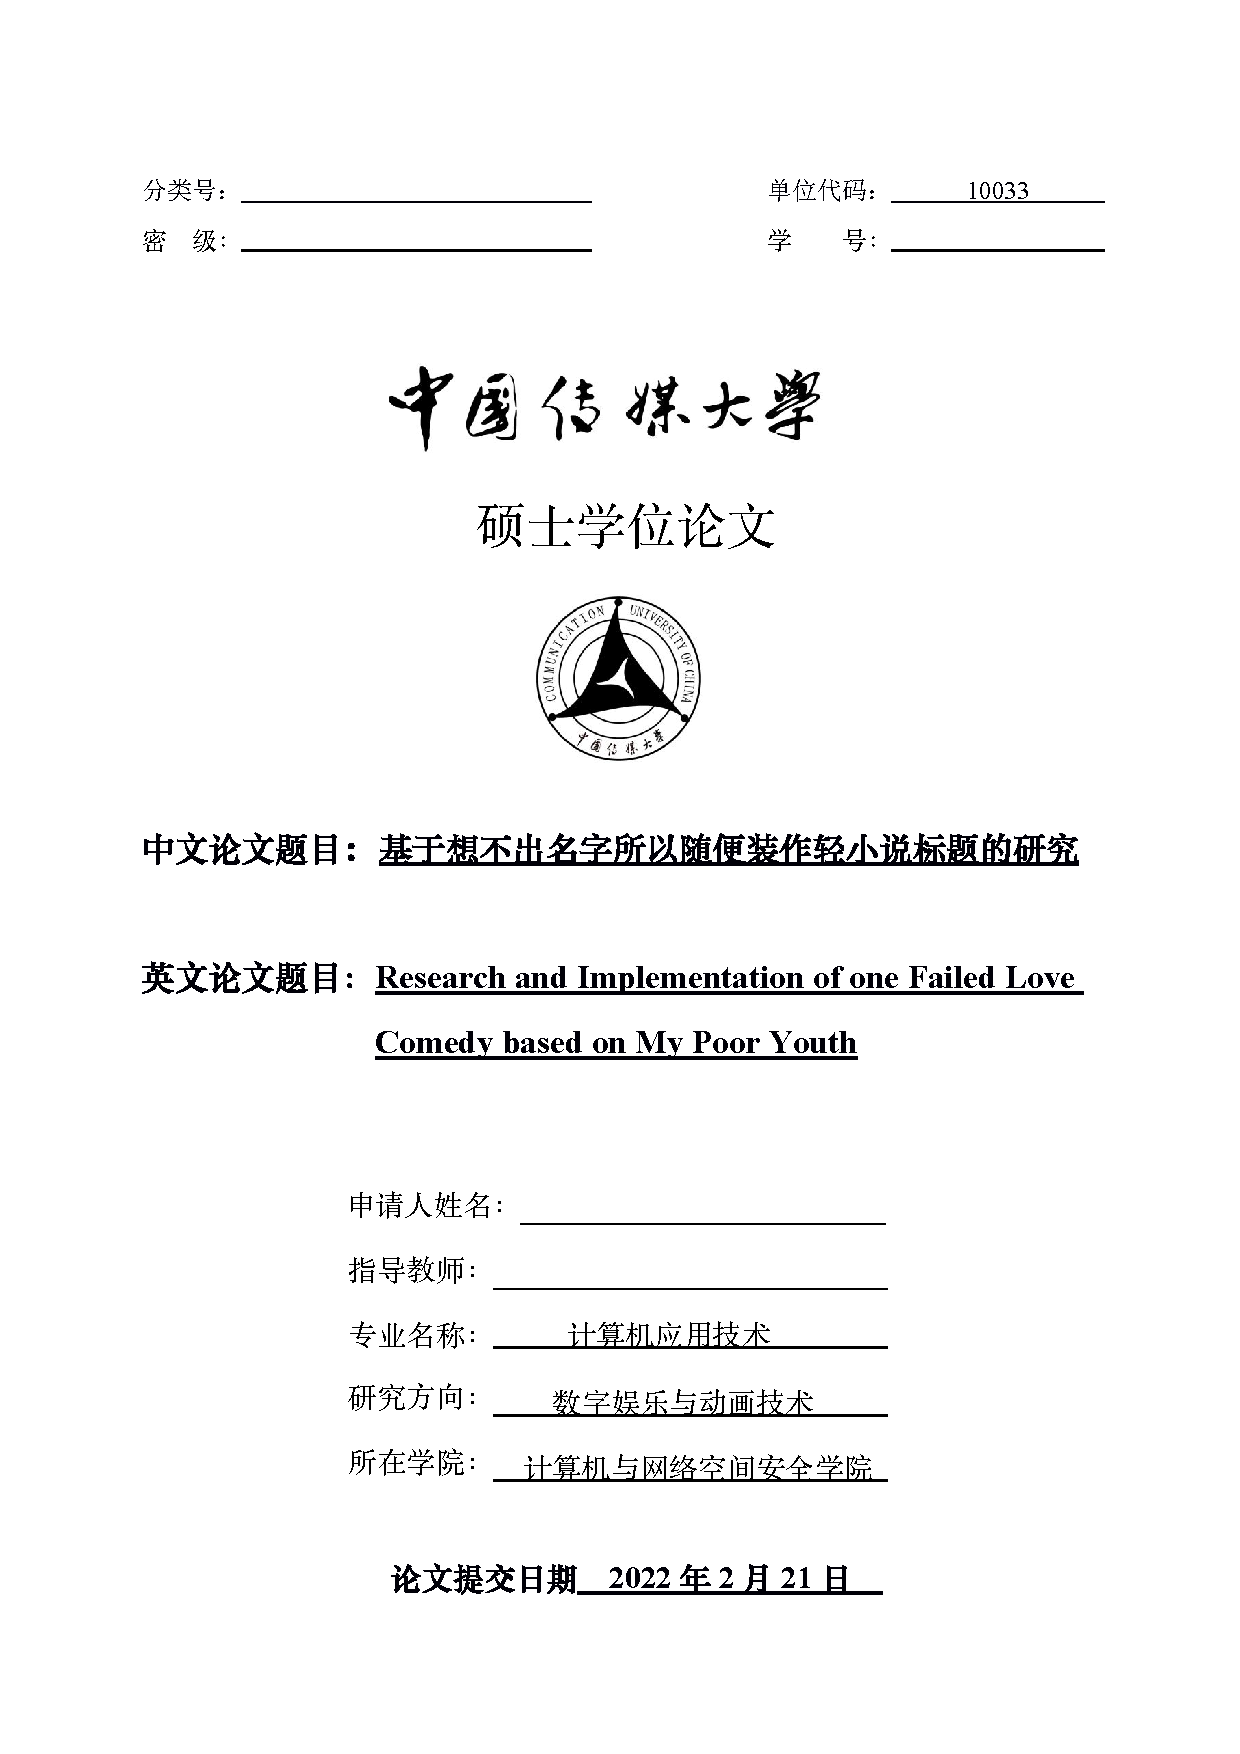
\includepdf[pages={1}]{cuc/cuc-thesis-cover.pdf}
% 盲审版本封面
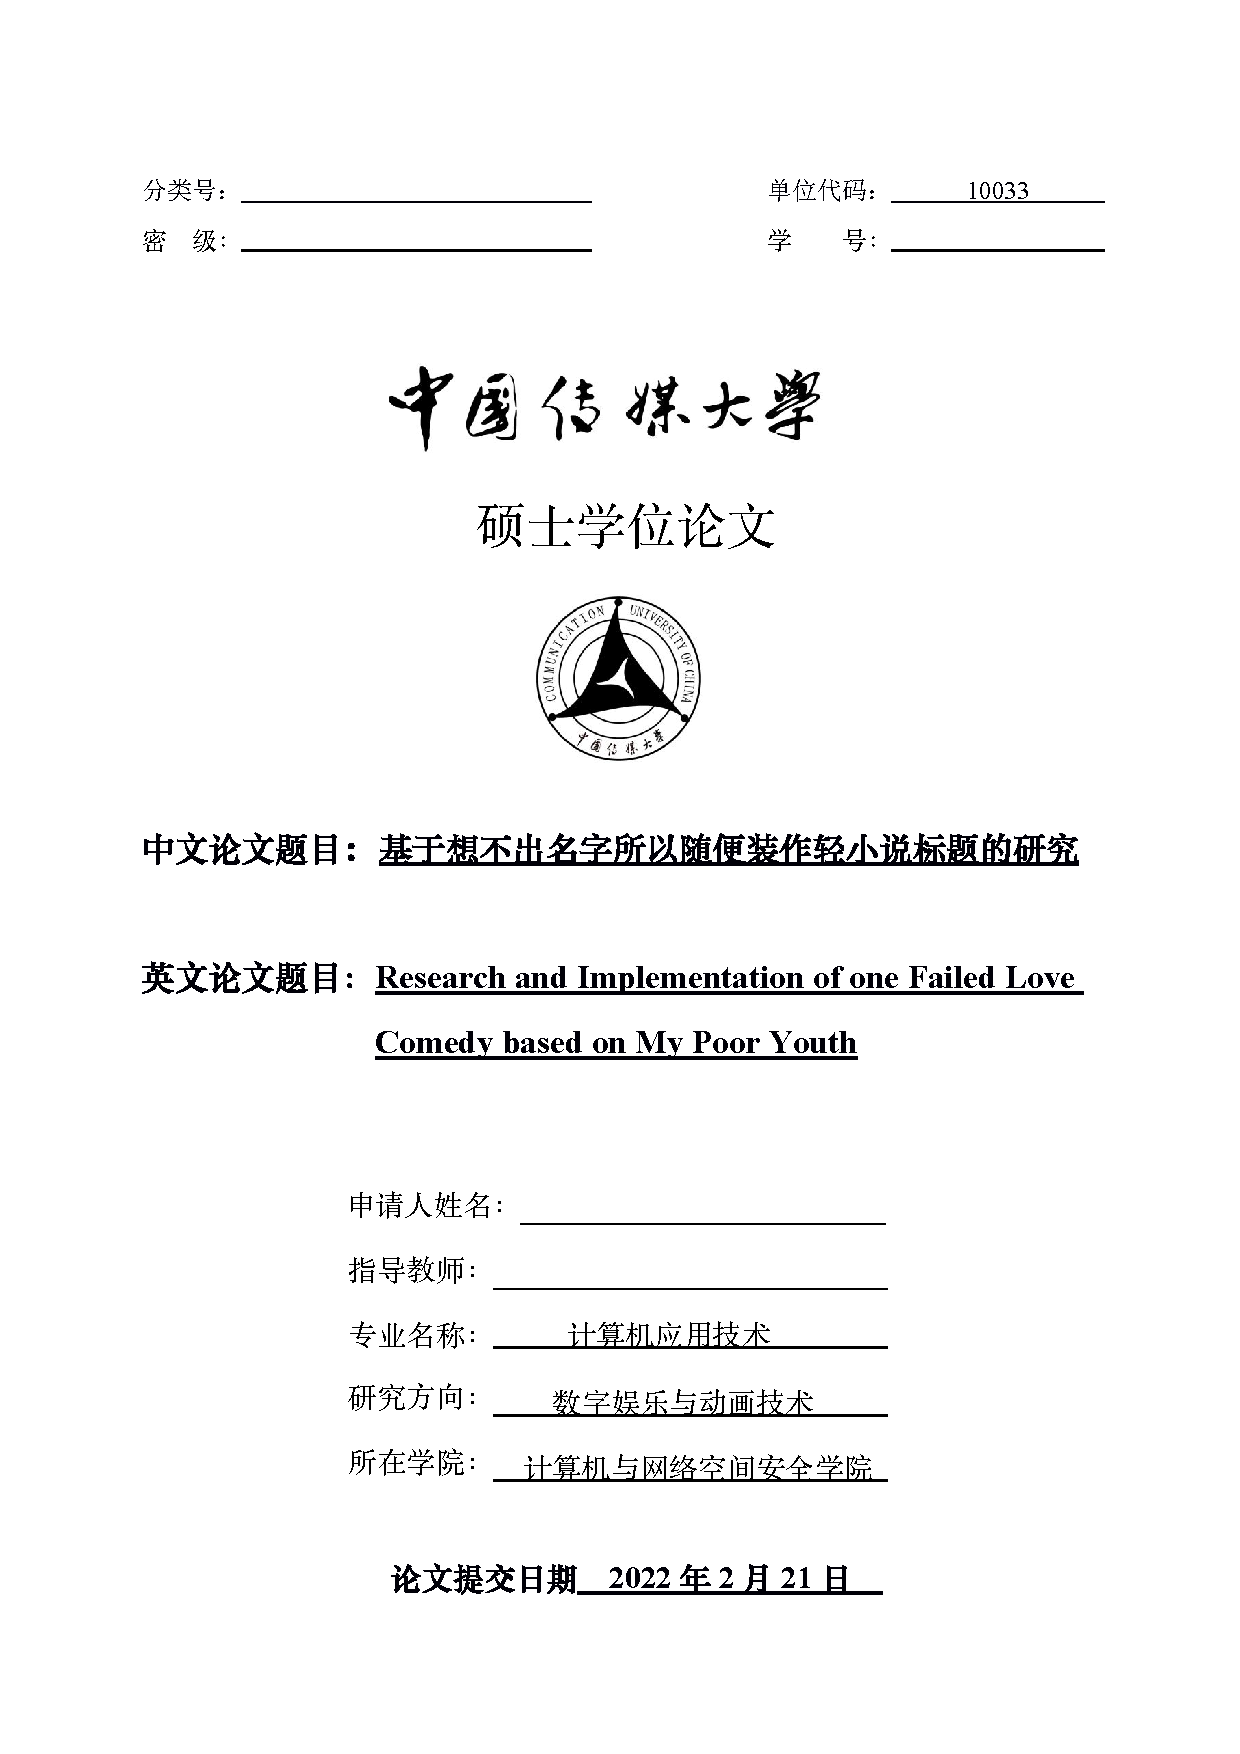
\includepdf[pages={1}]{cuc/cuc-thesis-cover-without-name.pdf}

\includepdf[pages={1}]{cuc/statement.pdf}

\frontmatter

% !TeX root = ../main.tex

% 中英文摘要和关键字

\begin{abstract}
  论文的摘要是对论文研究内容和成果的高度概括。
  摘要应对论文所研究的问题及其研究目的进行描述,对研究方法和过程进行简单介绍,对研究成果和所得结论进行概括。
  摘要应具有独立性和自明性,其内容应包含与论文全文同等量的主要信息。
  使读者即使不阅读全文,通过摘要就能了解论文的总体内容和主要成果。

  论文摘要的书写应力求精确、简明。
  切忌写成对论文书写内容进行提要的形式,尤其要避免“第 1 章……;第 2 章……;……”这种或类似的陈述方式。

  关键词是为了文献标引工作、用以表示全文主要内容信息的单词或术语。
  关键词不超过 5 个,每个关键词中间用分号分隔。

  % 研究生论文由于篇幅过长,通常可以划分几点
  % 主要工作内容如下:1. 2. 3.
  % \begin{enumerate}
  %   \item 
  %   \item 
  %   \item 
  % \end{enumerate}

  % 关键词用“英文逗号”分隔,输出时会自动处理为正确的分隔符,通常使用分号
  \thusetup{
    keywords = {关键词 1, 关键词 2, 关键词 3, 关键词 4, 关键词 5},
  }
\end{abstract}

\begin{abstract*}
  % 留空行缩进
  
  An abstract of a dissertation is a summary and extraction of research work and contributions.
  Included in an abstract should be description of research topic and research objective, brief introduction to methodology and research process, and summary of conclusion and contributions of the research.
  An abstract should be characterized by independence and clarity and carry identical information with the dissertation.
  It should be such that the general idea and major contributions of the dissertation are conveyed without reading the dissertation.

  An abstract should be concise and to the point.
  It is a misunderstanding to make an abstract an outline of the dissertation and words “the first chapter”, “the second chapter” and the like should be avoided in the abstract.

  Keywords are terms used in a dissertation for indexing, reflecting core information of the dissertation.
  An abstract may contain a maximum of 5 keywords, with semi-colons used in between to separate one another.

  有时候英文摘要会超过一页,分两页也是可以的(我看师兄是这样)

  % Use comma as separator when inputting
  \thusetup{
    keywords* = {keyword 1, keyword 2, keyword 3, keyword 4, keyword 5},
  }
\end{abstract*}


% 目录
\tableofcontents

% 插图和附表清单
% 本科生的插图索引和表格索引需要移至正文之后、参考文献前
\listoffiguresandtables  % 插图和附表清单
% \listoffigures           % 插图清单
% \listoftables            % 附表清单

% help
% include pdf https://stackoverflow.com/questions/2739159/inserting-a-pdf-file-in-latex
% \includepdf[pages=-]{myfile.pdf}
% \includepdf[pages={1}]{myfile.pdf}

% 正文部分
\mainmatter
\ctexset{
  chapter = {
    format      = \sffamily\sanhao,
  },
}
% \titleformat{\chapter}[hang]{\sanhao\heiti}{\thechapter}{1em}{}{\quad\quad}

% 论文一般共六章
% !TeX root = ../main.tex

\chapter{绪论}
\section{研究背景及意义}
渲染(Rendering)是根据场景信息和着色模型生成二维图像的过程,是计算机图形学的核心问题和最终目标。
渲染不仅能够应用于影视特效、虚拟仿真与电子游戏等文娱领域,还在教育、医学、军事等多个行业中发挥着关键作用。
根据产业调研报告\cite{beizhesi2024},2023年全球3D渲染和虚拟化软件市场规模已达92.82亿人民币。
为实现高质量渲染,场景通常以数字模型资产(Digital Model Asset)的形式存在,这些资产包含网格模型以及纹理贴图,
用以表示几何形状、反射属性等多种信息。不同的渲染技术则对资产的内容和格式提出了不同要求,二者紧密耦合。
这种耦合使得资产一旦制作完成,资产便与渲染技术形成了绑定,使得资产在渲染技术迭代或变化时难以兼容,
增加了项目开发的成本和风险。如图~\ref{fig:asset_rendering}中所示的皇冠即为数字资产,
当数字资产与渲染技术不匹配时,会产生预期之外的错误结果。
\begin{figure}[H]
  \centering
  \begin{subfigure}[t]{0.45\textwidth}
    \centering
    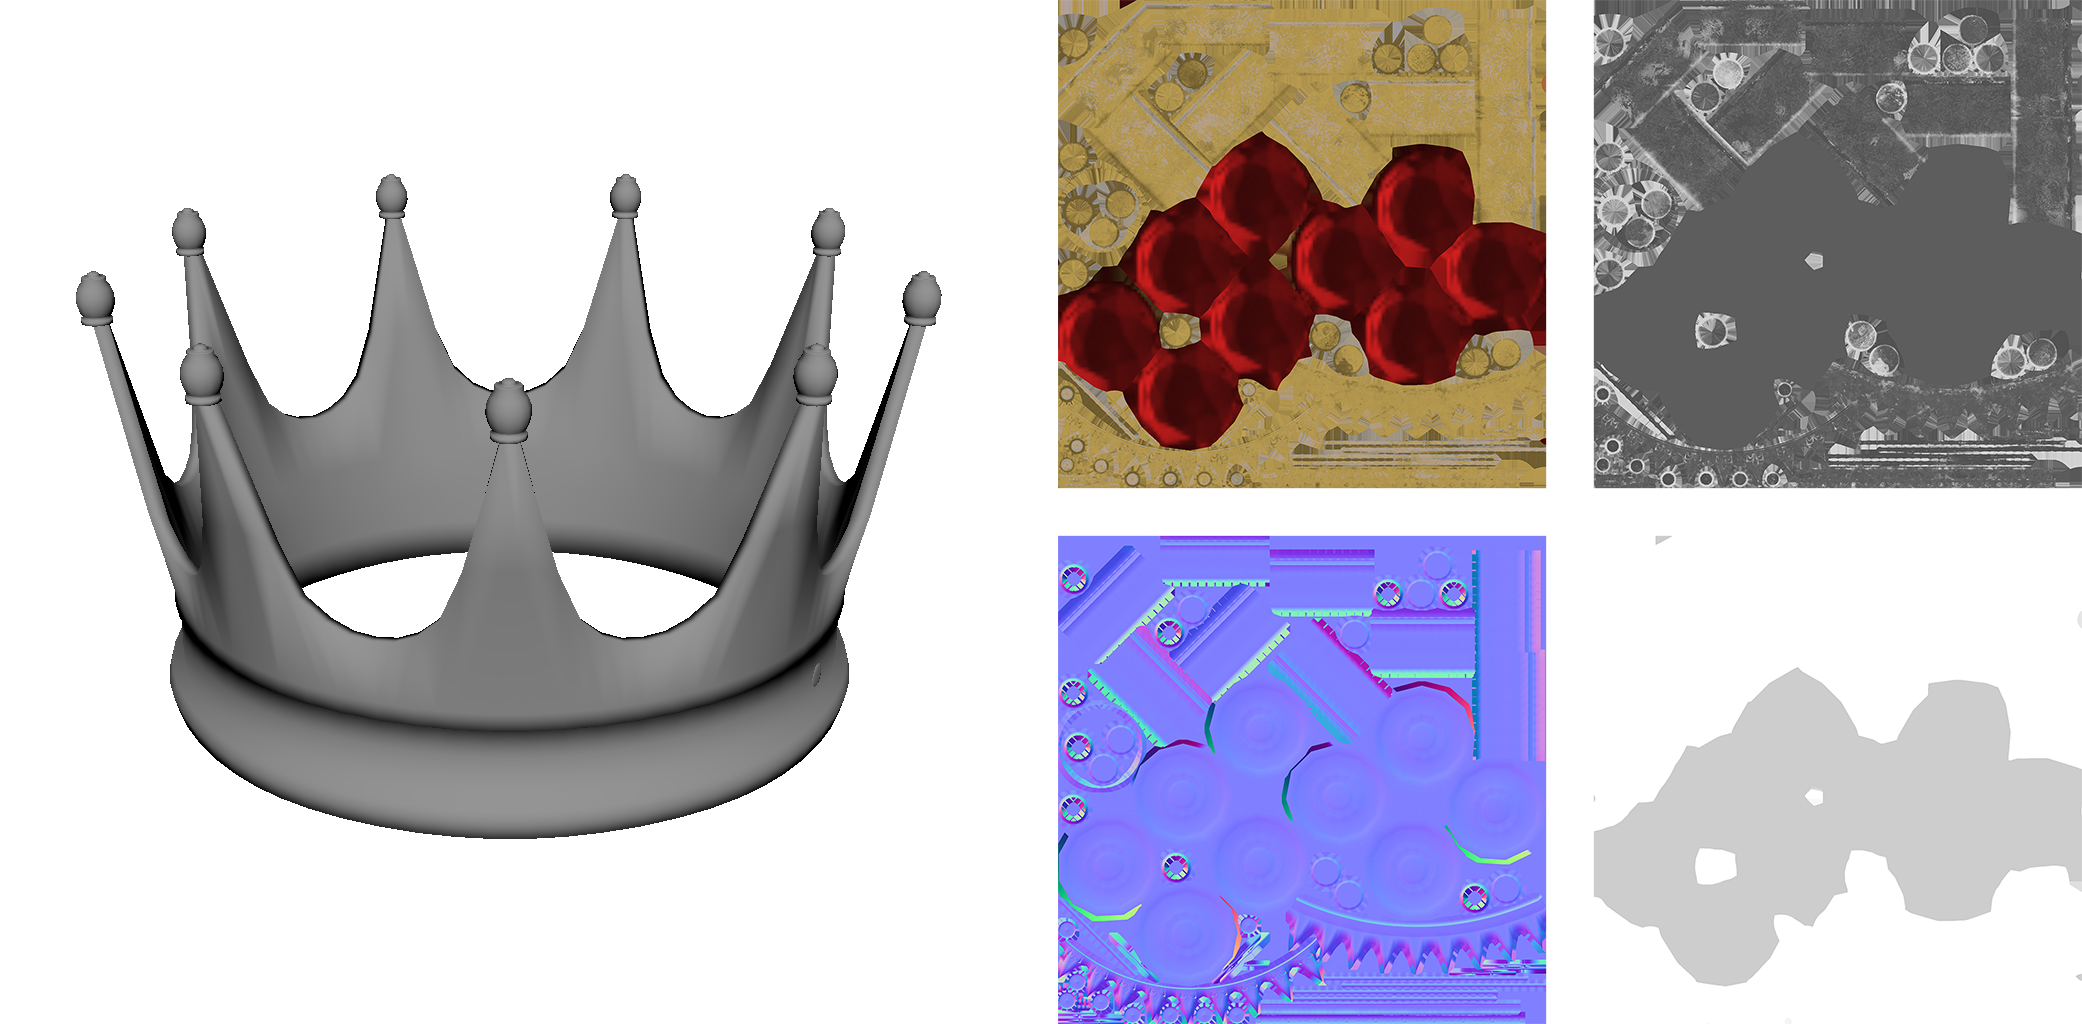
\includegraphics[height=3.5cm]{asset_error/digital_asset.png}
    \caption{数字资产皇冠}
  \end{subfigure}
  \hspace{3mm}
  \begin{subfigure}[t]{0.225\textwidth}
    \centering
    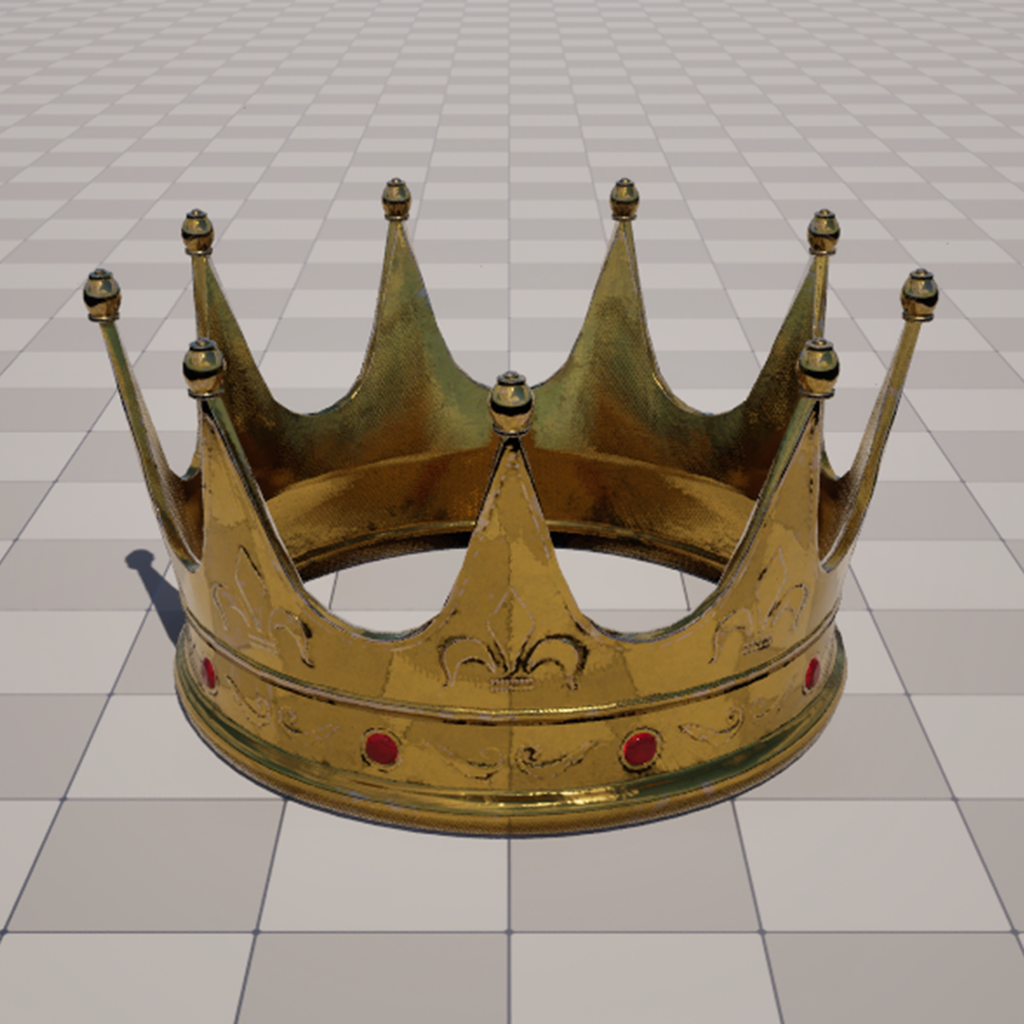
\includegraphics[height=3.5cm]{asset_error/correct.png}
    \caption{渲染结果}
  \end{subfigure}
  \begin{subfigure}[t]{0.225\textwidth}
    \centering
    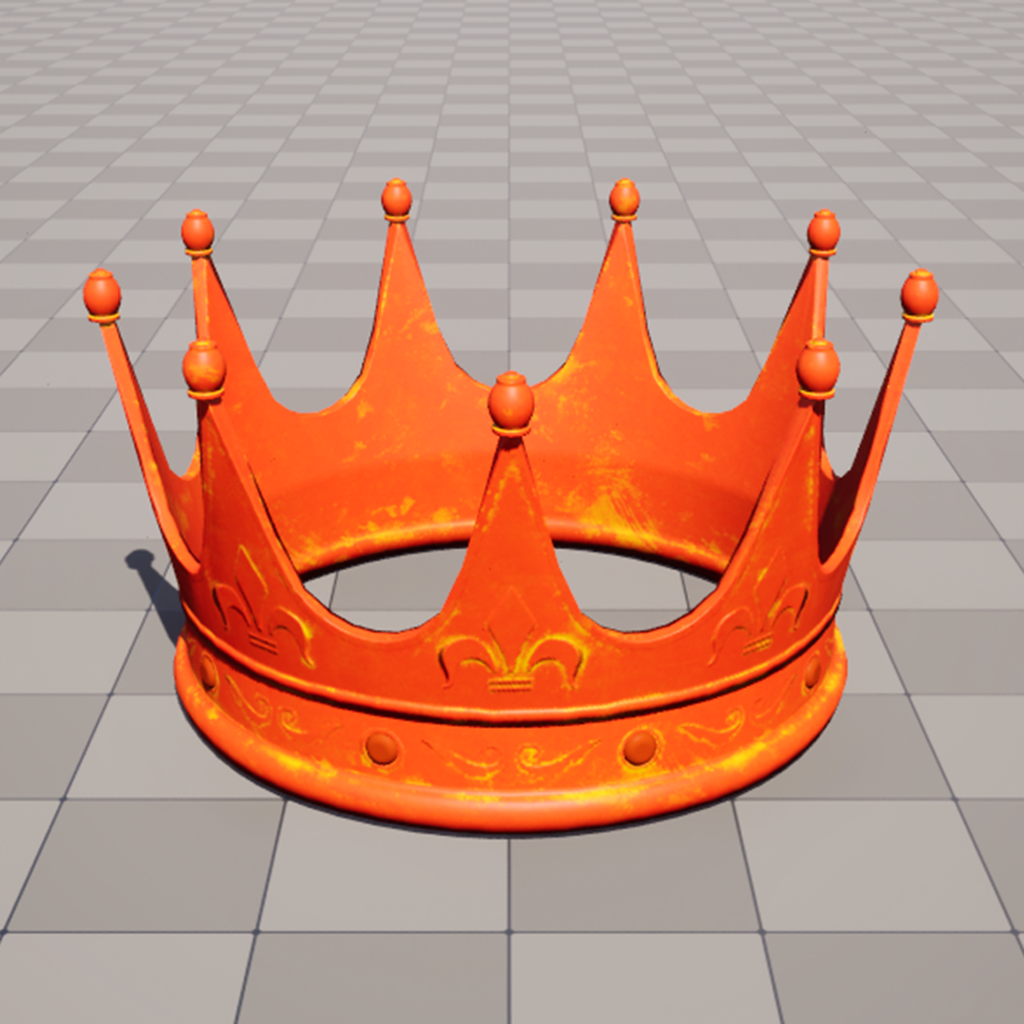
\includegraphics[height=3.5cm]{asset_error/error.png}
    \caption{渲染错误}
  \end{subfigure}
  \caption{数字资产及渲染}
  \label{fig:asset_rendering}
\end{figure}

为了尽可能减少二者耦合带来的负面影响,
在传统渲染管线中,不同领域和应用场景往往形成了各自的工作流(Workflow)。
工作流根据不同的渲染技术设计了不同的资产制作规范和后续编辑流程,在实际开发时,
资产只需严格遵循工作流的相应标准进行制作,即可保证能够兼容对应的渲染技术。

近年来,深度学习技术在计算机图形学领域崭露头角,
其中神经辐射场(Neural Radiance Fields,NeRF)作为一种新兴的三维场景表示方法,
通过隐式地将场景编码为连续的辐射场和体积密度场,实现了从稀疏二维图像重建三维场景的突破。
相较于传统方法,使用隐式连续表示的NeRF无需依赖显式的网格、点云或体素数据,避免了离散表示带来的伪影和内存开销,
展现了极高的通用性和灵活性。因此,本文旨在通过NeRF这种新颖的场景重建与表示技术,
解决数字资产与渲染技术之间紧密耦合的问题,为多种渲染工作流提供一种灵活、可编辑的数字资产表示方案。
本文的方法能够使得旧有资产不因技术不兼容被废弃,节省大量人力成本。
同时,也能允许开发者和创作者可以根据项目需求灵活切换工作流,提升创作自由度,
从而推动数字内容生产与渲染技术的发展。

\section{国内外研究现状}
\subsection{用于表征三维场景的神经辐射场}
NeRF通过多层感知机(Multilayer Perceptron,Coordinate-Based MLP)表示场景
并结合体积渲染生成新视角图像。传统方法
\cite{Waechter_2014, Mildenhall_2019, wu2020adversarial, Aliev_2020, Dai_2015}
通常采用显式的离散表示来构建三维场景,
但显式离散表示在利用梯度优化网格几何和拓扑结构时存在较大局限性,
因此研究者们逐渐转向基于连续体积的表示方案。
Mildenhall等人\cite{Mildenhall_2020}提出的NeRF采用了隐式的连续神经表示,用密度$\sigma$来描述场景几何形状,
通过光线步进在五维辐射场中计算出射辐射,从而实现图像渲染。
尽管这种方法在新视角合成上取得了令人印象深刻的成果,但由于体积渲染的固有局限,
NeRF生成的几何细节往往模糊不清,无法还原高频细节。

后续的相关研究主要集中在两个方向:一是探索改进的网络结构以保留更多场景细节
\cite{Chen_2022,Barron_2021,Barron_2022,dave2022pandora};
二是在不牺牲视觉质量的前提下,优化神经辐射场的训练与推理速度
\cite{Reiser_2021,Martin_Brualla_2021}。
同时,也有部分研究尝试采用基于表面的渲染方法,直接对物体表面进行优化。
例如,Wang等人\cite{10.5555/3540261.3542342}通过有向距离函数(Sign Distance Function,SDF)来表示形状,
并提出了从SDF到密度的无偏转换用以兼容NeRF的渲染框架。

然而,虽然以上这些方法在几何表示方法上各有不同,但仍然使用辐射场来描述场景的反射和光照信息。
辐射场将每一个着色点视为自发光光源,因此必须使用开销更高的体积渲染和光线步进生成图像,不兼容传统光栅化渲染器。
其次,这种编码方式使得NeRF相关研究易于完成新视角合成(Novel View Synthesis,NVS)任务,
但限制了NeRF在下游编辑任务或传统渲染器中的应用。


\subsection{神经辐射场的光照分解}

为了弥补上一节中所述的这些不足,Zhang等人\cite{Zhang_2021}和Boss等人\cite{Boss_2021}尝试将NeRF与可微渲染技术相结合,
在同一管线下联合优化,从而将辐射场信息分解为独立的几何形状、反射属性以及光照信息,以便在新的光照条件下实现重渲染或进一步编辑。
可微渲染旨在从观测图像中分离出物体的几何结构、材质属性和光照条件,将可微渲染融入NeRF框架的方案通常称为NeRF光照分解管线,
其研究重点在于如何准确地表示场景中的几何形状、反射属性和光照,以及如何选择合适的着色模型进行渲染。
下面将依次介绍现有方法在各个方面的研究现状。

\subsubsection*{(1)反射属性表示}

反射属性描述了光线在物体表面反射的特性。由于可微渲染为高度不适定(Highly ill-posed)的问题,
比如着色点颜色较亮既可能是由于粗糙浅色表面的漫反射产生,也可能是因为光滑深色表面的镜面反射导致,
因此早年间的工作\cite{Sato_1997, Zollh_fer_2015}中通常旨在恢复兰伯特(Lambertian)表面,即忽略掉高光反射属性。
近期工作中多使用基于物理的着色模型,其使用双向反射分布函数(Bidirectional reflectance distribution function,BRDF)
\cite{Cook_1981}来定义从反射属性到光照反射方式的计算过程。
NeRFactor\cite{zhang2021nerfactor}采用了数据驱动的BRDF,即将BRDF整体作为一个输出函数直接估计,
从而省略了将反射属性转换为BRDF的过程以降低误差。
Nerf2Mesh\cite{Tang_2023}则使用了近似的着色模型,抛弃了反射属性的物理意义,其管线的输出仅能使用特定的着色器。
这种方式虽然在一定程度上简化了问题,但导致输出的BRDF缺乏直观的物理意义,比如在传统渲染引擎中,
多采用参数化BRDF(如Disney Principled BRDF\cite{burley2012physically})使得材质编辑更加直观。
另外,由于基于物理的着色模型在真实感上的优越性能,所有的研究均采用了其或其近似。
但本文的目标旨在实现数字资产与渲染技术之间的解耦,数字资产可能需要多种着色模型进行渲染,
因此有必要对其进行扩展。为解决这些问题,本文提出的管线可以自定义不同的着色模型,
并通过材质管理的方式进行组织,以对应不同的工作流。这不仅使得输出结果能够直接用于传统渲染和后续编辑,
同时也实现了基于指定工作流的反射属性进行可微渲染的功能。

\subsubsection*{(2)几何形状表示}

几何形状表示的目标在于准确描述物体的空间结构和形态,为后续渲染与编辑奠定基础。
目前,大多数工作采用隐式神经表示来捕捉几何信息。虽然隐式神经表示在新视角合成任务中表现出色,
但其通常难以直接获得高质量的显式几何结构。其中,NeRD\cite{Boss_2021}维持了大部分原有的NeRF管线,
并且直接使用密度体积来表示几何形状。NeRFactor\cite{zhang2021nerfactor}在原有NeRF框架的基础上,
利用NeRF中的粗采样网络提取出神经表面,并在表面上进行后续的渲染步骤。
而其余大部分工作则根据NeuS\cite{10.5555/3540261.3542342}对NeRF的改进,使用SDF来表示几何形状,旨在还原更多高频细节,
如NeILF++\cite{Zhang_2023}、PhySG\cite{Zhang_2021}、NeRO\cite{Liu_2023}。然而这些工作使用的均为隐式神经表示,
主要面向重照明任务设计,而未专门针对下游编辑及传统渲染器渲染而优化。
针对这一局限,本文在NeRF光照分解任务中提出了一种基于混合几何表示方法的辐射场分解管线。
该方法能够将任意场景下的辐射场分解为显式表示的网格体,从而直接支持下游编辑任务与传统渲染技术。

\subsubsection*{(3)光照表示}

光照表示旨在描述场景中的光源分布、照明环境以及光与物体相互作用的方式,
是实现真实渲染的关键环节。NeRF2Mesh\cite{Tang_2023}认为复杂的着色过程会折损管线的几何重建效果,
因此不使用独立建模的光照表示。大多数现有方法对全局照明做出近似建模,
例如利用球面高斯(Spherical Gaussians,SGs)\cite{Boss_2021, Zhang_2021}、球面谐波(Spherical Harmonics,SHs)\cite{kuang2022neroic}、
低分辨率环境图点光照\cite{zhang2021nerfactor}。这些全局照明技术均能满足可微渲染的要求,但大部分工作未能有效处理阴影与可见性问题。
为了解决可微渲染中的光照无法高效表示阴影的问题,本文创新性地设计了一种基于条件输入的阴影调制模块,
能够将直接光照和环境光照根据阴影进行结合,并利用一个预训练的自动编码器定义了物理真实感和平滑的潜空间,
在不需要过高的额外计算成本的前提下提高了光照表示技术对阴影的处理能力。

\subsection{本文的主要贡献与创新}

本文设计的光照分解管线共为两个阶段,分别是利用NeRF建立神经辐射场,随后使用可微渲染分解神经辐射场,
最终获得指定标准的数字资产。本文的创新集中在1.2.2节所述的三个部分。针对光照表示,
本文设计了一种基于条件输入的阴影调制模块,并将其用于阴影感知的神经光照(Shadow-Aware Neural Light,SaNL),
创新地将直接光照和环境光照之间的关系融入其中,提升了光照方法的表示能力。在反射属性表示方面,
本文的管线允许根据工作流选择任意着色模型,赋予了管线输出任意工作流对应的数字资产的能力。
在几何形状表示方面,本文采用显式和隐式混合的表示方法,解决了现有研究仅能将结果用于重光照和新视角合成的问题,
实现了管线输出结果能够直接用于传统渲染和下游编辑。

总的来说,本文的贡献可以总结为:

\begin{itemize}
  \item 本文设计并实现了基于NeRF的数字资产解耦管线。该管线能够通过多张二维图像建立数字资产的神经表示,
  并以指定标准的工作流降维分解,解决了传统管线中数字资产与渲染技术之间的耦合,能够大幅节省游戏、影视等行业中的开发成本。
  \item 本文提出了阴影感知的神经光照表示SaNL,并使用即时渲染引擎和大量环境光照生成了阴影-光照数据集,训练了带有阴影关系、
  物理真实感和连续性等先验知识的神经光照表示。实验表明,在光照分解管线中,SaNL的表示效果优于现有的光照表示方式。
  \item 本文在管线中引入DMTet,实现了隐式和显式混合的几何形状表示方式,
  并设计了与其相匹配的损失函数以提高几何形状的分解效果。结合传统的纹理处理技术,
  本文的管线可以直接输出显式网格体表示的数字资产,无缝衔接了分解管线到传统的渲染任务或下游编辑。
\end{itemize}

\subsection{本文结构安排}
本节将介绍论文结构安排,包含每一章的主要内容和研究重点,以展示本文的工作思路和价值。

第1章,绪论。第1章首先介绍了本文工作的背景和意义,并进一步介绍了与本文研究相关的可微渲染研究、NeRF以及基于NeRF的光照分解。
本文根据以上研究的现状及本文目标,介绍了本文的创新点与主要贡献,并在最后一节阐述了全文的结构安排。

第2章,相关技术基础。在第2章中,本文将详细介绍工作内容相关的理论基础。为了理解NeRF和光照分解任务,
第2章首先将介绍深度学习的基本概念,然后深入讲解NeRF的理论基础。同时,第2章还介绍了传统管线中的概念及技术,
为本文管线与传统方法的对接打下了基础。最后,该章节将讨论可微渲染的理论基础,
为后续内容中进一步讲解本文研究提供理论支撑。

第3章,数字资产解耦管线的实现。第3章将介绍本文对数字资产解耦管线这一目标的具体实现。
本文首先通过分析选定了技术路线和工作内容。随后,本文解决了现有分解管线无法将输出直接用于传统渲染器的问题,
并引入了基于MLP的纹理来表示反射属性。最终本文实现了对数字资产解耦的目标,并完成了NeRF到传统渲染器和编辑的无缝衔接。
本文通过实验进一步证明了本文提出方法的适用性和可行性。

第4章,阴影感知的光照表示研究。第4章将介绍本文设计的用于表示光照的神经网络,
由于本文在第三章中观察到管线对阴影中的场景还原不加,因此创新性地设计了一种神经光照表示以解决该问题。
第四章从设计动机以及选用的基础结构出发,讲解本文创新性的阴影光照先验,并通过多个维度对该网络进行实验评估,以验证其有效性。

第5章,总结与展望。本章总结了全文的研究内容和成果,讨论了研究中的创新与不足,以及本文工作未来可能的改进方向和路线。


% !TeX root = ../main.tex

\chapter{相关技术基础}
本文工作开展在基于深度学习的神经辐射场之上,通过结合可微渲染实现了数字资产解耦管线,
致力于无缝对接传统渲染管线并解决其中的耦合问题。本章将介绍本文研究所必要的深度学习基础、
可微渲染理论基础、传统渲染管线介绍以及神经辐射场理论基础。

\section{深度学习基础}
【这里应该加点引言之类的】
\subsection{基于坐标的多层感知机}
多层感知机(Multilayer Perceptron, MLP)作为深度学习的基础模型,由感知机推广而来,
本质是一种前馈神经网络。MLP由多个神经元层组成,每个神经元的结构如图~\ref{fig:neuron}所示,其接收多个输入值,
并按照自身权重进行加权求和,接着,使用激活函数对其进行非线性变换,并将变换后的值传递给下一层神经元。

\begin{figure}[htb]
  \centering
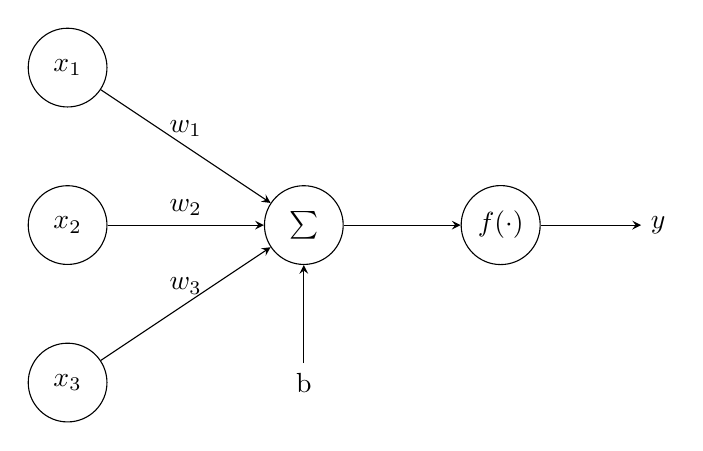
\begin{tikzpicture}[->,>=stealth, node distance=1.5cm, auto]
  % 定义输入节点
  \node[circle, draw, minimum size=1cm] (x1) at (0, 2) {$x_1$};
  \node[circle, draw, minimum size=1cm] (x2) at (0, 0) {$x_2$};
  \node[circle, draw, minimum size=1cm] (x3) at (0, -2) {$x_3$};

  % 定义偏置节点
  \node (bias) at (3, -2) {$\mathrm{b}$};

  % 定义神经元节点,内部写上激活函数(如 f(·))
  \node[circle, draw, minimum size=1cm] (sum) at (3, 0) {$\sum$};

  % 从输入节点到神经元的连线,并标注权重
  \draw (x1) -- node[midway, above] {$w_1$} (sum);
  \draw (x2) -- node[midway, above] {$w_2$} (sum);
  \draw (x3) -- node[midway, above] {$w_3$} (sum);
  % 从偏置节点到神经元的连线,标注偏置项
  \draw (bias) -- node[midway, below] {}(sum);

  % 定义神经元节点,内部写上激活函数(如 f(·))
  \node[circle, draw, minimum size=1cm] (activate) at (5.5, 0) {$f(\cdot)$};

  \node (y) at (7.5, 0) {$y$};

  \draw (sum) -- node[midway, below] {}(activate);
  \draw (activate) -- node[midway, below] {}(y);
\end{tikzpicture}
\caption{神经元的结构示意图}
\label{fig:neuron}
\end{figure}

多层感知机通过神经元从输入数据中学习到合适的参数权重和偏置项,利用激活函数将线性关系转化为非线性信号,
使得网络能够准确地完成各种分类或回归预测等方面的任务。这些信号从输入层通过一系列的隐藏层最终输出到输出层,
各层之间是完全连接的,具体如图~\ref{fig:mlp}所示:

\begin{figure}[htb]
  \centering
  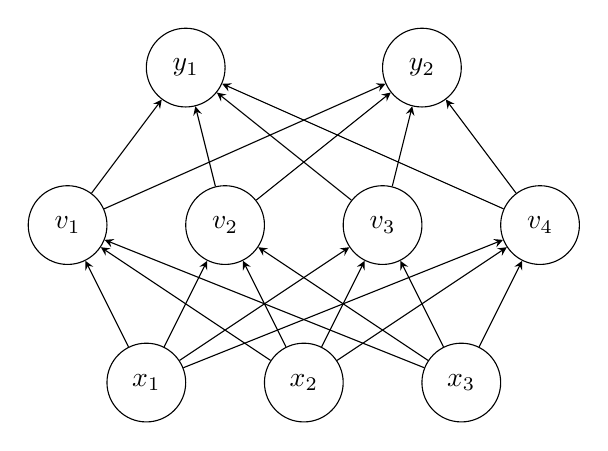
\begin{tikzpicture}[>=stealth, auto]

    % 定义公共变量
    \def\xspacing{2}      % 输入层和隐藏层的水平间距
    \def\layersep{2}       % 垂直层间距
    
    % 定义输出层特有的水平间距(可以调大该值)
    \def\outputxspacing{3} % 输出层水平间距
  
    % 输入层:3个节点
    \foreach \i in {1,...,3} {
      \pgfmathsetmacro{\xpos}{(\i-2)*\xspacing};
      \node[circle, draw, minimum size=1cm] (x\i) at (\xpos, 0) {$x_{\i}$};
    }
  
    % 隐藏层:4个节点
    \foreach \i in {1,...,4} {
      \pgfmathsetmacro{\xpos}{(\i-2.5)*\xspacing};
      \node[circle, draw, minimum size=1cm] (v\i) at (\xpos, \layersep) {$v_{\i}$};
    }
  
    % 输出层:2个节点,使用新的水平间距
    \foreach \i in {1,...,2} {
      \pgfmathsetmacro{\xpos}{(\i-1.5)*\outputxspacing};
      \node[circle, draw, minimum size=1cm] (y\i) at (\xpos, 2*\layersep) {$y_{\i}$};
    }
  
    % 连接输入层到隐藏层(全连接)
    \foreach \i in {1,...,3} {
      \foreach \j in {1,...,4} {
        \draw[->] (x\i) -- (v\j);
      }
    }
    
    % 连接隐藏层到输出层(全连接)
    \foreach \i in {1,...,4} {
      \foreach \j in {1,...,2} {
        \draw[->] (v\i) -- (y\j);
      }
    }
  
  \end{tikzpicture}
\caption{多层感知机的结构示意图}
\label{fig:mlp}
\end{figure}

根据通用近似定理\cite{Hornik_1989},只要给予网络足够多的神经元,MLP即可以任意精度逼近紧致集上的连续函数,
这一理论奠定了MLP作为函数逼近器的数学基础。然而,传统MLP多用于处理向量化特征(如图像分类中的扁平化像素),
其输入空间通常缺乏明确的几何语义。基于坐标的多层感知机(Coordinate-based MLPs)则突破了这一局限,
通过将空间坐标直接作为网络输入,并引入傅里叶坐标编码(Fourier Positional Encoding)
进行频域编码\cite{tancik2020fourier},
实现了对连续场函数的隐式建模,从而开创了三维几何与信号表示的新范式。

具体而言,直接使用原始坐标作为输入会导致 MLP 呈现明显的频谱偏差问题\cite{pmlr-v97-rahaman19a}。由于网络倾向于优先学习低频信号,
导致网络难以捕捉三维几何中的高频细节(如表面纹理、尖锐边缘等)。为此,研究者提出利用傅里叶坐标编码,
将 $d$ 维坐标 $\mathbf{x}\in\mathbb{R}^d$ 通过傅里叶基函数投影至高维空间。
傅里叶坐标编码可以由公式\eqref{eq:fourier_encoding}表示:
\begin{equation}
\gamma(\mathbf{x})=\left[\sin\left(2^0\pi \mathbf{x}\right),\cos\left(2^\pi \mathbf{x}\right),\ldots,\sin\left(2^{K-1}\pi \mathbf{x}\right),\cos\left(2^{K-1}\pi \mathbf{x}\right)\right]
\label{eq:fourier_encoding}
\end{equation}
其中 $K$ 为预设的频率层级,通过指数增长的频率项构造多尺度频带。
这种傅里叶坐标编码(Fourier Positional Encoding)使MLP能够显式访问不同频段的几何特征,
有效解决了频谱偏差问题。在神经辐射场(NeRF)等典型应用中,该技术被证明是实现高质量三维重建的关键因素。

\subsection{激活函数}

通过上文的介绍我们知道,在多层神经网络中,隐藏层仅能进行线性变换,因此仅由隐藏层组成的线性模型只
能拟合输入和输出之间的线性关系,无法处理非线性问题。为了增强模型的非线性表示能力,可以使用激活函数来加入非线性因素。
由于不同类型的激活函数对提高网络的非线性表示能力不同,所以针对不同的任务需要选择适合的激活函数。
当基于坐标的多层感知机使用ReLU等常见激活函数时,网络同样易于出现上文所述的频谱偏差问题。
ReLU激活函数的基本表达式如公式\eqref{eq:relu}所示:
\begin{equation}\label{eq:relu}
\text{ReLU}(x)=
\begin{cases}
x, & x>0,\\[1mm]
0, & x\leq 0.
\end{cases}
\end{equation}
它在 $x>0$ 时具有线性函数的特征,而在 $x\leq 0$ 时则恒定为0,这样可以使部分神经元的输出为0,
从而实现网络的稀疏性,缓解过拟合问题。此外,ReLU激活函数计算速度快,导数简单。
但是,这种单侧抑制机制虽能提升模型稀疏性,但其频谱响应呈现强烈的低频偏好:ReLU的导数在正区间为常数1,
负区间为0,其傅里叶变换能量集中于低频段。当应用于坐标输入时,ReLU的频谱偏差会抑制网络对高频几何细节
(如曲面曲率、纹理梯度)的捕捉,导致重建结果过度平滑。

为突破这一限制,Sitzmann等人\cite{sitzmann2020implicit}提出了SIREN(Sinusoidal Representation Networks),该网络创新性地采用正弦函数作为核心激活函数。
正弦激活函数可以由公式\eqref{eq:siren}表示:
\begin{equation}\label{eq:siren}
\phi_i(x_i)=\sin\Bigl(\omega_0\,W_i\,x_i+b_i\Bigr)
\end{equation}
其中 $\omega_0$ 为可学习的频率缩放因子。正弦激活函数通过周期性振荡特性,为神经网络引入频谱调制能力。
相较于ReLU,正弦函数的无限可微性及其导数的非零特性,使得网络可通过链式法则传递高频梯度信号,
避免频谱能量衰减。而权重矩阵 $W_i$ 与频率因子 $\omega_0$ 共同调节输入信号的频域分布,
使网络自适应平衡低频轮廓与高频细节的建模(如图\ref{fig:siren_compare}所示)。

\begin{figure}[htb]
  \centering
  % 这里可以控制图片宽度比例
  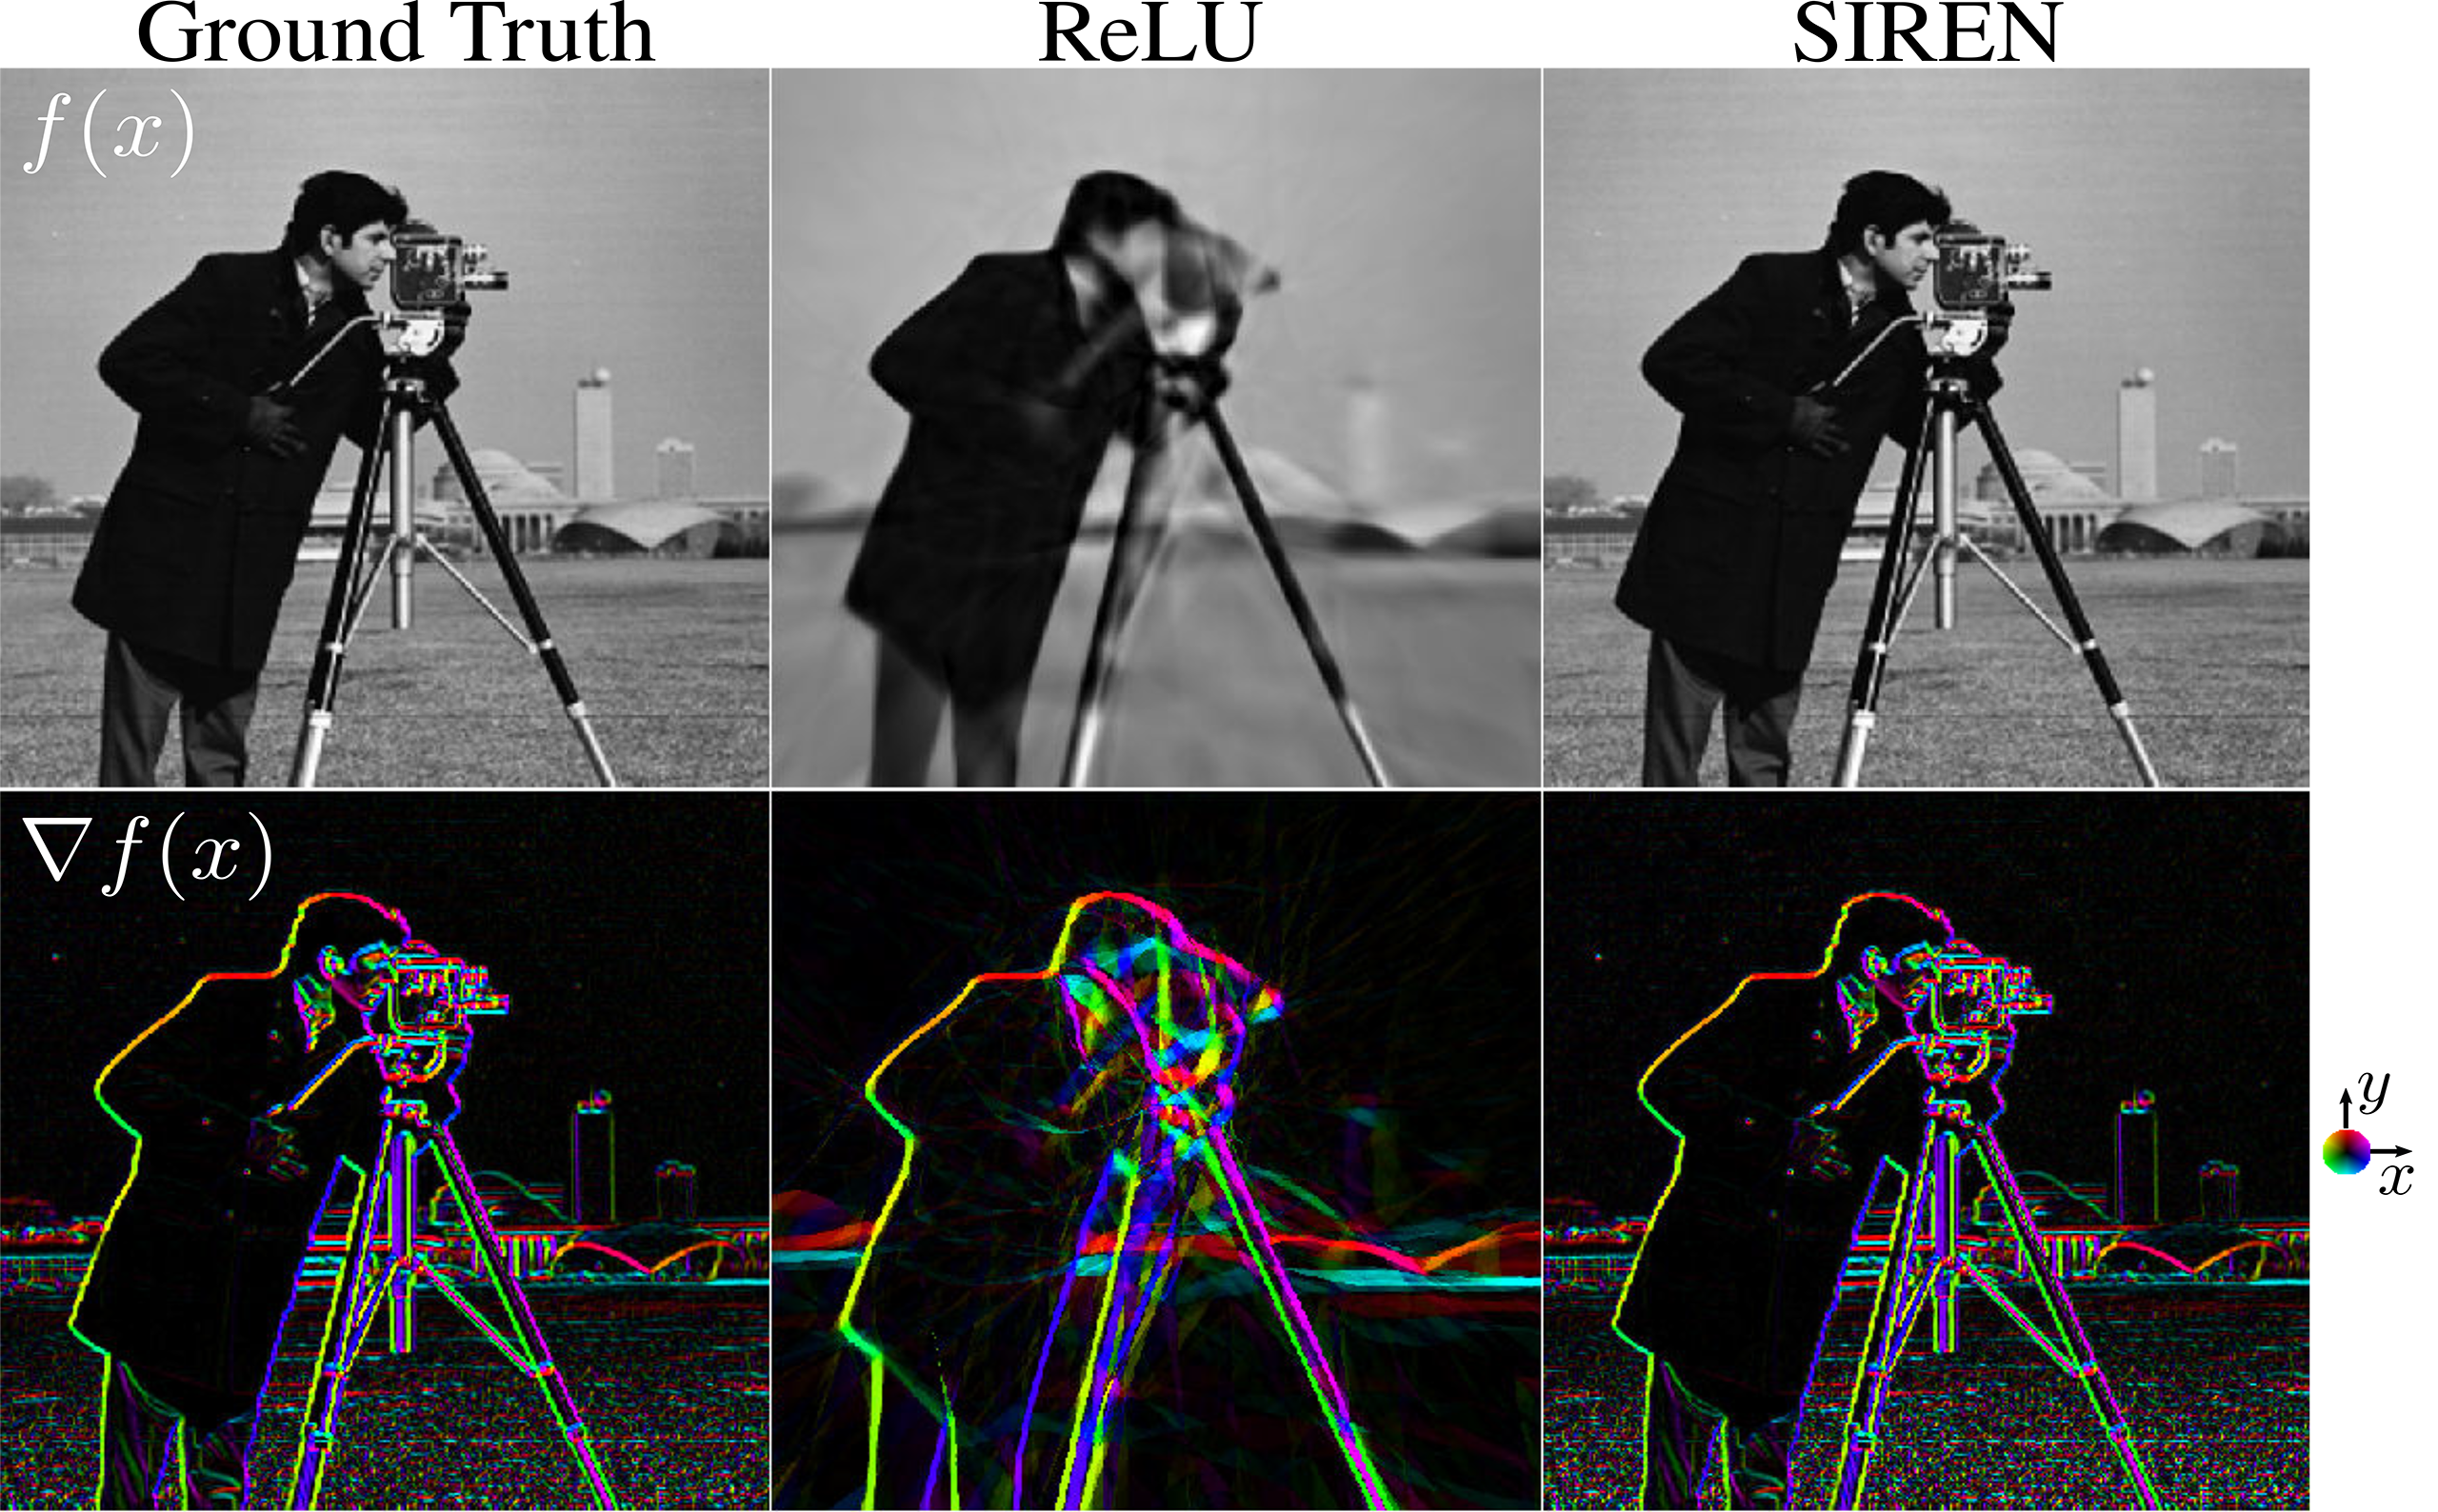
\includegraphics[width=0.6\linewidth]{Siren.png}
  \caption{激活函数对比\cite{sitzmann2020implicit}}
  \label{fig:siren_compare}
\end{figure}

实验\cite{sitzmann2020implicit}表明,采用正弦激活的MLP在3D形状重建任务中可将PSNR提升3-5 dB,
收敛速度加快5倍。这一突破性进展验证了激活函数频谱特性对隐式神经表示质量的决定性作用,
也为物理场仿真、微分方程求解等需高阶导数连续性的任务提供了新范式。

\subsection{损失函数}
【】【】这里还没写。

\subsection{自动编码器}
自动编码器(Autoencoder)作为深度学习中重要的无监督学习架构,其核心思想源于对生物感知系统中信息压缩与重建机制的仿生模拟。
该架构由对称的编码器(Encoder)与解码器(Decoder)网络构成,通过最小化输入数据与重建输出之间的差异,
迫使网络学习数据本质特征的紧凑表示。从数学角度来看,自动编码器可以看作是一种将高维数据转换为低维表示的工具:
编码器 $\mathcal{E}:\mathcal{X}\rightarrow\mathcal{Z}$ 将输入数据 $x\in\mathbb{R}^D$ 投影至 $z\in\mathbb{R}^d$ ,
解码器 $\mathcal{D}:\mathcal{Z}\rightarrow\mathcal{X}$则试图从潜在编码重构原始输入 $\hat{x}=\mathcal{D}\left(\mathcal{E}\left(x\right)\right)$,
其优化目标可以由公式\eqref{eq:ae_loss}给出:
\begin{equation}\label{eq:ae_loss}
\min_{\theta,\phi}E_{x\sim p_{\mathrm{dt}}}\Bigl[\bigl|x-\mathcal{D}_\phi\bigl(\mathcal{E}_\theta(x)\bigr)\bigr|^2\Bigr]
\end{equation}
其中$\theta$和$\phi$分别代表编码器与解码器的参数。这种方法不仅能在没有标注的数据中发现内在结构,而且在特征提取、
降维和去噪等应用中取得了很好的效果。早期的研究\cite{Hinton_2006}发现,当网络使用非线性激活函数并对低维空间进行一定限制时,
其能够有效地提取数据中的关键因素,比如在图像处理中自动识别边缘、纹理等重要视觉元素。

同时,自动编码器在处理复杂的光照估计与可微渲染问题时也有重要的作用。自动编码器的优势在于能够从高维数据中提取出最关键的特征,
并捕捉数据内在的低维结构。当我们面对真实世界的光照环境时(例如256\times256分辨率的环境贴图),
传统方法直接在原始像素空间进行优化会遇到三个问题:其一,像素数可能高达数百万,导致梯度下降等优化算法容易陷入局部最优;
其二,光照参数需要符合辐射度非负、能量守恒等物理规律,而仅仅依靠人工设计的正则项通常难以完全表达这些约束;
其三,实际光照中存在一些低维特性(如色温分布、主要光源的方向偏好),但要显式建立这些规律需要精确的先验知识。

因此,在可微渲染的任务里,自动编码器能够利用数据压缩的特性,通过编码器将高维环境贴图压缩到一个较低维的潜在空间,
构建出紧凑的光照参数表示,从而大大降低了优化问题的维度。同时,解码器将潜在向量映射回满足物理规律的光照配置,
确保优化过程中始终处于可行解范围内。这种“压缩-重建”机制实际上学习了一个数据驱动的光照投影操作,使得光照估计问题可以转化为在一个
平滑且低维的空间中进行高效搜索。例如,在同时优化物体材质和光照时,只需要调整潜在空间中的少量参数,就能获得物理上合理的光照重构,
而无需直接处理数百万维的像素数据。

\section{传统渲染管线}
本节介绍传统渲染管线的相关知识,为本文针对工作流进行光照分解补充相关背景知识。传统渲染管线中,
数字资产通常由网格体和多张纹理贴图组成,其中,网格体表达了数字资产的几何形状,纹理贴图和各类参数表达了数字资产表面不同的光学属性。
本节将介绍数字资产的制作和渲染过程,并解释数字资产与着色模型之间存在的耦合关系。

\subsection{渲染方程}


渲染方程(Rendering Equation)是计算机图形学中描述光与物体表面交互的基础方程之一。
由Kajiya等人于1986年提出\cite{Kajiya_1986},它为物体表面的光照计算提供了一个物理上合理的模型,
广泛应用于真实感渲染和计算机图像生成中。渲染方程通过描述光从场景中的光源到达表面并反射到观察者的过程,
计算表面点的辐射亮度(radiance)。具体计算过程如公式\eqref{eq:rendering_equation}:
\begin{equation}
  \label{eq:rendering_equation}
  L_o\left({\bf{x}},\omega_o\right)=\int_{\upOmega}f_r\left({\bf{x}},\omega_i,\omega_o\right)\cdot L_i\left({\bf{x}},
  \omega_i\right)\left(\omega_i\cdot\mathbf{n}\right)\,\mathrm{d}\omega_i
\end{equation}
其中,$L_o\left({\bf{x}},\omega_o\right)$表示从表面点$\bf{x}$沿观察方向$\omega_o$看到的辐射亮度,
$L_i\left({\bf{x}},\omega_i\right)$是从入射方向$\omega_i$到达表面点$\bf{x}$的光源辐射亮度,
$f_r\left({\bf{x}},\omega_i,\omega_o\right)$是BRDF,
它决定了光线从入射方向$\omega_i$到反射方向$\omega_o$的散射方式,且依赖于表面的材质属性。
$\left(\omega_i\cdot\bf{n}\right)$表示入射光与表面法线$\bf{n}$的点积,代表表面与光源的接触程度,
而$\mathrm{d}\omega_i$是入射光方向的微小立体角元素。

渲染方程的核心思想是通过积分所有可能的光源对表面反射的贡献,计算出最终的观察光照。
其在实际应用中能够模拟多种光照现象,包括漫反射、镜面反射、折射以及其他复杂的光学效应。
然而,尽管渲染方程具有强大的表达能力,但其高计算成本使得在实时渲染中难以直接应用。
因此,许多基于渲染方程的模型需要进行简化或近似,以实现高效的图像生成。

\subsection{着色模型}

着色模型(Shading Model)是基于渲染方程的简化或近似,通常用于图形学中的实时渲染。其主要目标是通过简化光的反射过程,
使得渲染计算更加高效。通过引入一定的数学公式和参数设置,着色模型能够近似真实世界中的光照现象,
从而生成具有理想真实感或艺术效果的图像。着色模型的核心是描述光线与物体表面相互作用的数学函数,
输入通常包括入射光线、视角、表面法线以及材质属性(如漫反射颜色、镜面反射强度、粗糙度等),
输出则是某一点处的最终光照颜色或亮度。常见的着色模型包括:

\fourthtitle{1}基于物理的着色模型

这些模型遵循物理定律,精确描述光照现象,通常依赖于双向反射分布函数。
例如,Cook-Torrance模型[29] 通过微表面分布函数、几何遮蔽因子和Fresnel反射等参数,精确地模拟了金属和非金属表面的反射行为。
基于物理的着色模型能够较为准确地模拟光的反射、折射和散射过程,生成更为真实的视觉效果。

\fourthtitle{2}经验性(非物理)着色模型

这类模型通常采用简化或经验公式来近似光照计算,
代表性的有Blinn-Phong模型和Lambertian模型。尽管它们并不完全遵循物理定律,
但通过经验参数(如光泽度、反射系数等)的调控,依然能够生成具有一定真实感的光照效果。
由于计算复杂度较低,经验性模型广泛应用于实时渲染或资源受限的场景。

\subsection{工作流}
工作流(Workflow)在计算机图形学中指的是一套标准化的参数与贴图生成流程,它定义了如何结合和组合各类材质参数和贴图,
以表述数字资产表面不同的光学属性。简言之,工作流决定了如何构建数字资产的表面属性,使其能够符合特定的着色模型的计算需求。
因此,选择适当的工作流对于高效且精准地表达材质的视觉效果至关重要。

工作流与着色模型之间具有紧密的耦合关系,每种工作流设计都对应着特定的着色模型,这些模型通过接收由工作流生成的参数和贴图,
进行光照计算与视觉效果渲染。不同的工作流基于不同的物理或经验性模型,表达表面特性的方式也有所不同。
本节介绍三种工作流兼具了基于物理的以及非物理的着色模型,并且仍在现代渲染引擎和项目中广泛使用。

\fourthtitle{1}金属度工作流

该工作流利用金属度(Metallic)贴图区分金属与非金属区域,使用粗糙度(Roughness)描述表面的粗糙程度。
由于该工作流直接描述物体表面的金属性质,因此渲染效果更易符合预期。在该工作流的数字资产中,共使用三张纹理:
基础色(Albedo)纹理在金属材质中表示镜面反射颜色,而在非金属中表示漫反射颜色,记为$\mathbf{b}$;
金属度(Metallic)贴图区分金属与非金属区域,记为$m$;粗糙度(Roughness)描述表面的粗糙程度,记为$r$。

金属度工作流可以使用微表面模型的Cook-TorranceBRDF完成计算,该模型将渲染方程中的$f_r$分为漫反射项$f_d$
以及高光反射项$f_s$:
\begin{equation}\label{eq:cook-torrance}
f_r=f_s+f_d.
\end{equation}

漫反射项$f_d$表示表面上从所有方向散射的光,通常使用Lambertian反射模型表示,即光照强度与表面法线和入射光方向的夹角无关,
只与入射光的方向有关,计算过程如下:
\begin{equation}\label{eq:lambertian}
f_d=\frac{1-m}{\pi}
\end{equation}

高光反射项$f_s$表示光线在光滑表面上按镜面反射规律反射的部分,通常依赖于入射光和观察方向与表面法线之间的角度关系,
可以被表示为:
\begin{equation}\label{eq:specular}
f_s(\omega_o,\omega_i)=\frac{D({\bf{h}};r)\cdot F(\omega_o,{\bf{h}};{\bf{b}},m)\cdot G(\omega_i,\omega_o,{\bf{h}};r)}
{4\cdot({\bf{n}}\cdot\omega_i)\cdot({\bf{n}}\cdot\omega_o)}
\end{equation}

其中,$D$是法线分布函数(Normal Distribution Function, NDF),$F$是菲涅尔(Fresnel)反射项,$G$是几何遮蔽(Geometry)
项,$\bf{h}$是半角向量,$\bf{n}$为表面法线。针对$D$项、$F$项以及$G$项的计算,不同的研究中针对着色风格均提出了多种实现,
接下来本文将介绍主流的几种计算方法。

在大多数渲染器中,$D$项通常使用GGX\cite{walter2007microfacet}计算,使用粗糙度控制其锐利程度:
\begin{equation}\label{eq:D_ggx}
D({\bf{h}};r)=\frac{r^2}{\pi\Bigl(({\bf{n}}\cdot{\bf{h}})^2(r^4-1)+1\Bigr)^2}
\end{equation}

同时,为了在可微渲染中使用,$D$项也可以由球面高斯(Spherical Gaussians)近似计算为:

\begin{equation}\label{eq:Dsg}
D_{\rm{SG}}({\bf{n}};r)=\frac{1}{\pi r^4}\exp\Biggl(\frac{2}{r^4}\Bigl({\bf{n}}\cdot{\bf{h}}-\mathbf{1}\Bigr)\Biggr)
\end{equation}

F项可以根据Schlick等人\cite{schlick1994inexpensive}的研究近似计算,由如下公式给出:
\begin{equation}
  \label{eq:F}
  F(\omega_o,{\bf{h}};{\bf{b}},m)=F_0+\bigl(1-F_0\bigr)\Bigl(1-(\omega_o\cdot{\bf{n}})^5\Bigr)
\end{equation}
其中,$F_0$ 项可以通过公式\eqref{eq:F_0}表示为:
\begin{equation}
  \label{eq:F_0}
  F_0=0.04(1-m)+{\bf{b}}m
\end{equation}

最后,G项可以根据Heitz等人\cite{heitz2014understanding}的研究使用Smith联合遮蔽阴影函数(Smith Joint Masking-Shadowing),计算方式如下:
\begin{equation}
  \label{eq:G}
  G(\omega_i,\omega_o,{\bf{n}};r)=G_{\rm{GGX}}(\omega_i\cdot{\bf{n}})\,G_{\rm{GGX}}(\omega_o\cdot{\bf{n}})
\end{equation}
其中,$G_{\rm{GGX}}$ 由公式\eqref{eq:G_ggx}计算:
\begin{equation}
  \label{eq:G_ggx}
  G_{\rm{GGX}}(z)=\frac{2z}{(2-r^2)z+r^2}
\end{equation}

\fourthtitle{2} Specular工作流

该工作流通过镜面反射(Specular)贴图和漫反射(Diffuse)贴图直接控制材质表面的镜面反射与漫反射颜色,
通过光泽度(Glossiness)贴图控制镜面反射的强度和大小。Specular工作流与描述表面物理性质的Metallic工作流不同,
该工作流更为灵活,可以为材质单独指定不同的镜面反射率。例如蓝色的陶瓷材质对于Metallic工作流可能需要设置部分违反物
理直觉的值才能实现,但是使用Specular工作流时可以直接调整出真实的反射表现。

在计算上,Specular工作流也使用Cook-Torrance BRDF,区别在于部分计算方式不同。首先,对于上文中公式\eqref{eq:F}所述的菲涅尔项$F$,
Specular工作流替换了其中的$F_0$:
\begin{equation}\label{eq:F0_spec}
F_0=\bm{c}_s
\end{equation}
随后,在计算漫反射项$f_d$时不再根据金属度进行插值,而是使用菲涅尔项$F$作为插值系数:
\begin{equation}\label{eq:diffuse_spec}
f_d=\frac{1-F}{\pi}
\end{equation}
这种计算方式使得即使Specular允许艺术家自由分配镜面反射和漫反射的表现,也保证了能量守恒,尽量避免出现物理不真实的问题。

\fourthtitle{3} Blinn-Phong工作流

该工作流基于经验性着色模型(Blinn-Phong模型),通常依赖漫反射(Diffuse)、高光反射(Specular)贴图来模拟光照效果。其中高光反射参数在公式中实现了高光部分的近似计算,以光斑的形式提供近似的光滑观感,高光反射项$f_s$计算方式如下:
\begin{equation}\label{eq:specular_BlinnPhong}
f_s=\max(\mathbf{n}\cdot \mathbf{h},0)^\alpha
\end{equation}
漫反射部分使用Lambertian经验模型。总体的计算方式可以通过如下公式表示:
\begin{equation}\label{eq:diffuse_BlinnPhong}
f_d=\frac{1}{\pi}
\end{equation}

尽管该工作流并不严格遵循物理法则,且渲染效果无法与基于物理的模型相比拟,但它的计算开销较小,无需复杂的积分,适合用于对渲染效率有较高要求且对真实感要求较低的项目,非常适合于手机等移动端设备。

\subsection{数字资产与着色模型的耦合}
从前文的介绍可以看出,数字资产与着色模型之间存在着紧密的耦合关系。每种工作流预设了特定的参数组织方式,
并且与相应的着色模型或反射模型密切绑定。例如,金属度工作流通常与基于物理的Cook-Torrance BRDF模型配合使用,
以确保在渲染时,金属与非金属材质在光照下的反射行为符合物理规律。如果工作流中预设的参数与着色模型所需的参数不匹配,
可能导致最终渲染结果与预期不符,进而影响数字资产的效果和视觉质量。

尽管这种耦合关系使得数字资产的制作流程更加直观,并且提高了资产制作的效率与规范性,但它也存在一定的局限性。
特别是在开发过程中,这种严格的绑定要求数字资产必须按照特定规范进行制作,从而限制了技术迭代的灵活性。
在一些大型项目或长期维护的项目中,若需要升级着色模型,通常会导致大量现有数字资产需要重新制作或手动转换,
消耗了巨大的时间和经济成本。

为了解决这一问题,本文提出了一种新的解决方案:设计并实现一套端到端的数字资产管线,
通过将数字资产表示为神经辐射场(NeRF),并根据指定的工作流进行分解,从而打破数字资产与着色模型之间的紧密耦合。
该管线能够使数字资产在保持物理准确性和艺术效果的同时,具有更高的灵活性和可扩展性,进而为着色模型的快速迭代和工作流的适配提供支持。

\section{可微渲染理论基础}
传统渲染过程将三维场景描述转换为二维图像,但在标准计算机图形学管线中,该过程通常是不可微的,
如遮挡判断与离散三角形选择的操作并不连续,导致难以获得有效的梯度信息。
这一特性限制了渲染在基于梯度优化的机器学习和计算机视觉任务中的应用。
可微渲染(Differentiable Rendering, DR)是一种将传统渲染过程与梯度优化方法相结合的新兴技术,
其核心理念是致力于实现从三维场景到二维图像的映射过程中的可微性,从而能够通过误差反向传播直接优化场景参数。
因此,这一技术在计算机视觉和三维重建等任务中具有重要价值。

可微渲染的核心目标是计算渲染图像相对于场景参数的梯度,即$\tfrac{\partial I}{\partial \upPhi}$,
其中$I$是渲染图像,$\upPhi$包含几何、材质、光照和摄像机参数。由于渲染过程中的某些操作(如光栅化、可见性计算和光照建模)
通常具有离散性或复杂的非线性特性,使得计算其导数较为困难,不同的可微渲染方法针对这些挑战提出了解决方案。
接下来,本文将分别介绍可微渲染中常见的光照表示技术和几何形状表示方法。

\subsection{基于图像的照明与近似}
可微渲染中的光照表示需要满足多个关键需求,包括精确性、可微性以及对复杂光照环境的高效建模。
在这一背景下,基于图像的光照(Image Based Lighting, IBL)技术成为广泛应用的选择。
在完整的渲染方程\eqref{eq:rendering_equation}中,常规离散光源被表示为$L_i(\mathbf{x},\omega_i)$,
其在计算时需要考虑着色点的位置,而在IBL中则假设环境处于“无限远”状态。也就是说,
任何一处的光源所发出的光线都是平行的,而且其辐射强度在空间中是均匀的。这种假设使得对于场景中任何一点,
入射光的强度仅依赖于光线的方向,而不依赖于具体的位置,仅需计算$L_i(\omega_i)$

此外,可微渲染需要光照模型在物理上保持连续性,从而支持梯度的计算与传播。IBL采用环境贴图存储光照数据,
通过球面投影方式在空间中形成自然的连续分布。相比离散的点光源,环境贴图能够以较高的分辨率捕捉光照场景中的细节,
同时在可微渲染的优化过程中避免了不连续性对梯度的影响。这种连续性确保了光照参数的可导性,
从而能够在可微渲染中有效优化与光照相关的参数。

除此之外,Hill等人\cite{Hill_2014}引入了分裂和近似(Split-Sum Approximation),并将其应用于现代即时渲染中,以进一步降低计算量。
分裂和近似方法主要目的是将原本公式\eqref{eq:rendering_equation}中需要在半球上计算的高维积分
拆分成两个易于预计算并在运行时快速查表获得的部分,从而大大降低计算成本,
同时获得足够精确的视觉效果。分裂和近似的思想可以由公式\eqref{eq:int_approx}表示:

\begin{equation}
  \int f(x)g(x){\rm{d}}x\approx \int{f(x){\rm{d}}x} \int{g(x){\rm{d}}x}
  \label{eq:int_approx}
\end{equation}

公式\eqref{eq:int_approx}将两个函数乘积的积分近似为两个函数积分的乘积,
当该思想应用于渲染方程中的镜面反射项时,则镜面反射项可以通过以下形式近似计算:

\begin{equation}
  L(\omega_o)\approx 
  \int_{\upOmega}{f(\omega_i\cdot{\bf{n}}){\rm{d}}\omega_i}
  \int_{\upOmega}{L_i(\omega_i)D(\omega_i,\omega_o)(\omega_i\cdot{\bf{n}}){\rm{d}}\omega_i}
  \label{eq:L_omega_o_approx}
\end{equation}

其中,第一项表示白色环境光照的镜面BSDF积分,取决于参数$\cos{\theta}=\omega_i\cdot{\mathbf{n}};$
第二项表示法线分布函数与入射光的积分,当采用环境贴图技术时,该项可以被视作按照不同的表面粗糙度对环境贴图进行过滤,
也可以通过Mipmap等技术预先进行计算。通过IBL技术以及分裂和近似,着色时的计算量得以大幅减少,
因此这两项技术对于可微渲染任务来说不可或缺。

但是,IBL技术在实现过程中依赖的假设简化了光照建模的复杂性,将环境光表示为来自球面上的均匀方向分布,
而忽略了光源与场景之间的距离关系、遮挡关系。这种假设在许多传统渲染任务中是合理的,但在可微渲染中,
这种假设限制了IBL对光照空间分布的表达能力,尤其在涉及局部光照变化的场景中。例如,在阴影区域中,
光线受到物体遮挡后显著衰减,而IBL由于假定光照均匀分布于无限远,难以精确捕捉遮挡效应,
从而导致阴影处的光照表示不准确。此外,IBL的假设忽略了离散光源直接光的影响,无法精确建模光源位置与着色点之间的几何关系。
因此,在传统渲染中由点光源或聚光灯直接形成的高频光照效应(如强烈的高光或投影)也难以通过IBL实现。

\subsection{几何表示}
几何表示是可微渲染的关键组成部分, 用于描述场景的几何形状。用于可微渲染的良好几何表示应该捕获
局部几何细节并表示具有任意拓扑的对象,同时还具有内存和计算效率,以便在交互式应用程序中进行快速推理。
根据实现原理,表示形式主要可以分为传统图形学中的显式表示和结合了深度学习和神经网络的隐式表示两类。

\fourthtitle{1} 显式表示

显式表示方法通过直接定义物体表面的几何元素实现对三维形状的描述,主要包括网格(Mesh)、点云(Dense Cloud)
和符号距离函数(Signed Distance Function, SDF)三种典型形式。其中,网格表示通过顶点、边和面构成的多边形网格刻画物体形状,
其顶点可附加纹理坐标、法线及颜色等属性,具有直观可编辑的特点,且能高效利用图形硬件的加速能力。
然而,实际应用中不同存储格式的兼容性问题常需额外处理,且网格拓扑结构的刚性约束限制了其在重建任务中对高频细节的还原能力。
点云表示通常由激光扫描或立体视觉设备直接生成,具有采集便捷、密度可调的优势,但因缺乏显式拓扑关联,
其直接渲染效果粗糙且编辑灵活性不足,难以满足高质量实时交互需求。
相比之下,符号距离函数(SDF)通过为空间点赋予到表面的带符号距离值,既能以连续函数形式捕捉几何细节,
又可实现紧凑的数据存储,但其计算复杂度与空间分辨率的关系需通过特定算法优化。

\fourthtitle{2} 隐式表示

隐式表示通过参数化模型间接定义几何形状,近年来以神经隐式表示为核心的研究取得了显著进展。
该类方法利用神经网络$F(P_i^{xyz})$预测三维点$P_i^{xyz}\in\mathbb{R}^3$的几何属性,
其内存消耗与空间分辨率无关,理论上支持无限分辨率的表面重建。典型实现包括三种范式:
占据概率模型将几何描述转化为二分类问题,通过神经网络预测点$P_i^{xyz}$位于物体内部的概率以定义形状边界;
透明度建模则直接学习空间点的透明属性,既可表征半透明物体,也可近似非透明体的占据概率;
水平集方法将物体表面定义为隐式函数$F(P_i^{xyz})=0$的解集,通过距离函数的符号区分内外空间,
在复杂几何重建中兼具精度与计算效率优势。尽管神经隐式表示存在训练耗时、采样效率低等挑战,
但其参数化特性与拓扑无关性为高精度复杂几何建模提供了突破性解决方案,
尤其在细节还原和动态拓扑适应方面展现出独特潜力。

\fourthtitle{3} 混合表示
现有的隐式神经表示方法难以将生成结果直接用于下游编辑等任务,而传统的显式网格体在重建效果上有所折损,
而Shen等人\cite{shen2021deep}提出了深度行进四面体(Deep Marching Tetrahedra,DMTet),
该方法结合了SDF与网格体表示的优点,并且计算过程可微,适用于可微渲染管线。

DMTet使用离散的SDF表示每个顶点相对于原位置的偏移量,通过可微行进四面体层
(Differentiable Marching Tetrahedra Layer,MT)将SDF转换为三角形网格,
使得该技术能够基于SDF进行优化,并直接转换为网格体。由于这种转换能够在网络优化期间进行,避免了
传统隐式表示在管线后额外转换为网格表示时引入误差的情况。同时,DMTet也解决了直接使用网格体进行优化时,
网格体拓扑相对固定、无法表示细微高频细节的情况。

DMTet的优化过程如下,当给定一个四面体网格(Tetrahedral Grid),对于网格中的每个顶点v,
DMTet学习对应的SDF值$s$和变形向量$\Delta\mathbf{v}$,随后根据学习到的SDF值生成三角形面,
构成网格体。

DMTet从SDF生成三角形面的计算方式如图\ref{fig:dmtet_calc}所示,其中,标量$s$表示SDF值,
顶点$v_i$的位置$v_i^\prime$根据$s_i$的偏移进行更新,两个相邻顶点$v_i$和$v_j$之间的顶点$v_{ij}$通过线性插值进行计算。

\begin{figure}[htbp]
  \centering
  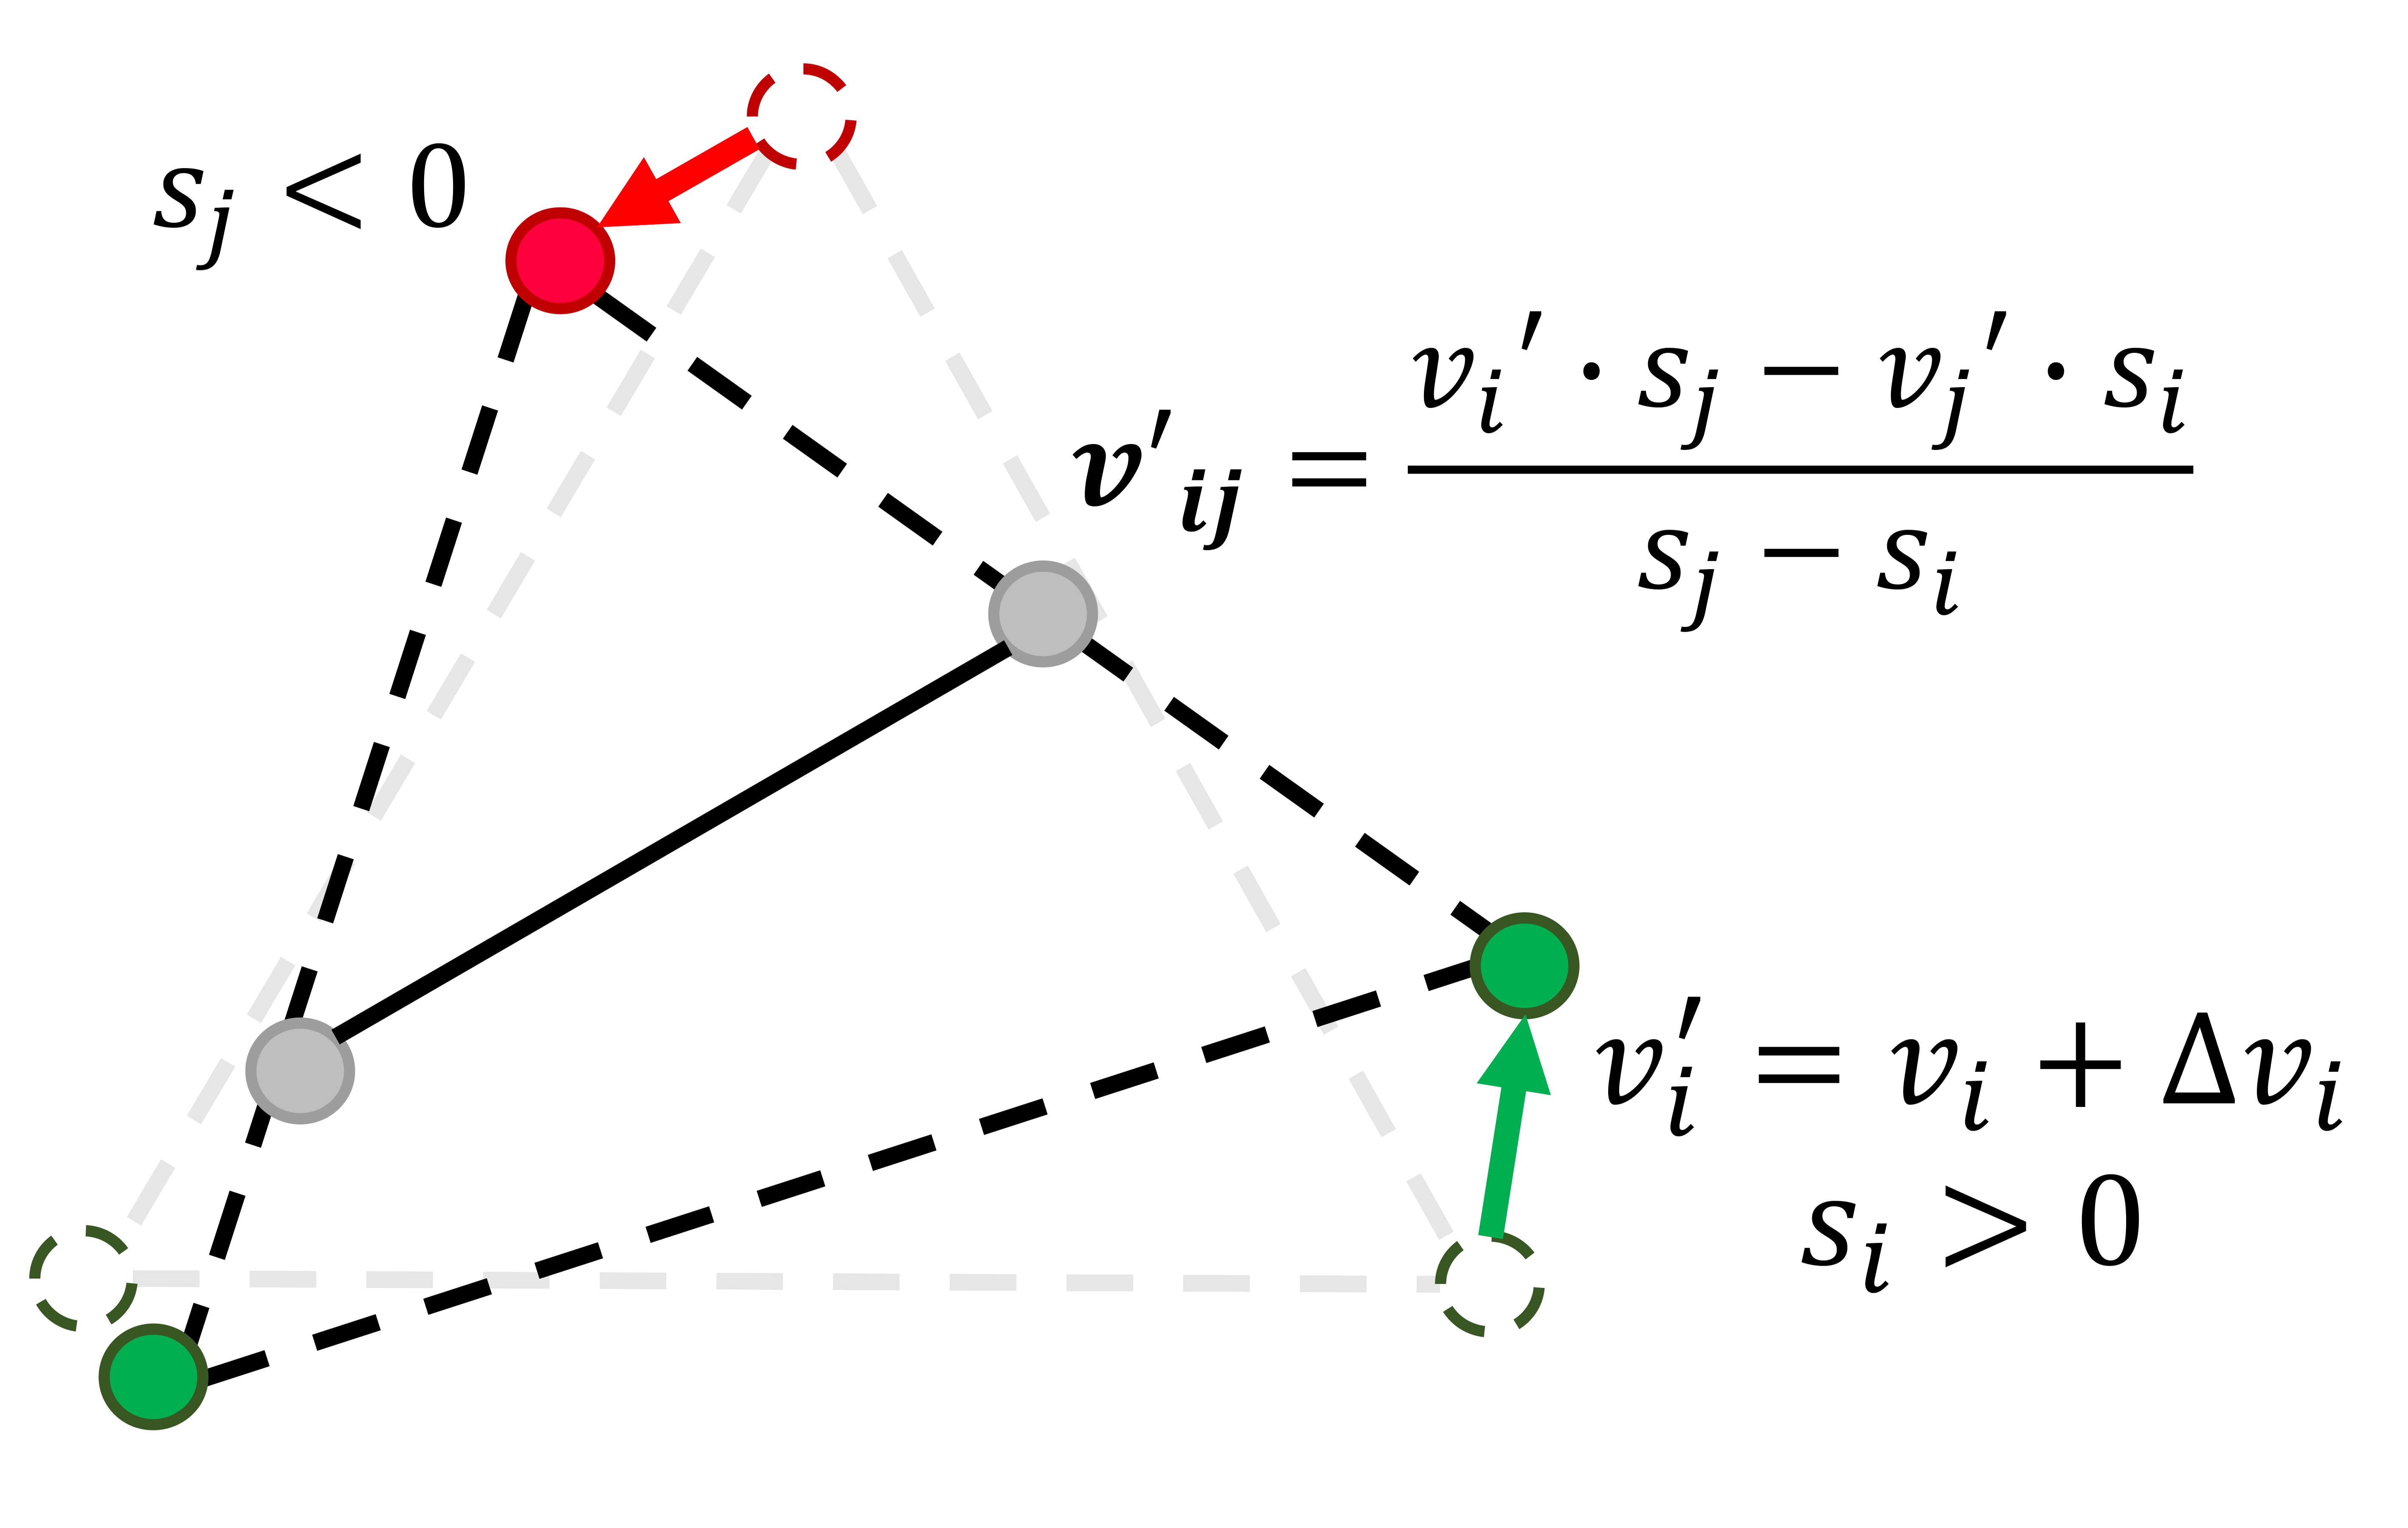
\includegraphics[width=0.5\textwidth]{SDFtoMesh.png}
  \caption{DMTet计算三角形面的过程}
  \label{fig:dmtet_calc}
\end{figure}

\section{NeRF理论基础}

NeRF技术通过融合辐射场建模与可微分体积渲染,实现了仅凭多视角二维图像即可优化三维场景隐式表示的技术突破。
作为基于坐标的多层感知机在视觉任务中的扩展,NeRF通过分析一组从多个视角捕获的二维图像,
能够推断出场景的三维几何结构和视觉外观。这种方法的核心优势在于其能够合成全新的视角图像,
即便这些视角在原始图像集中并未直接观测到。NeRF技术的突破性在于它对光线在三维空间中的传播进行建模,
利用深度神经网络学习和推理光线与物质相互作用的复杂过程,从而实现对场景的髙度真实感渲染。
这不仅在计算机视觉领域引起了革命性的变革,也为图形学的发展开辟了新的研究方向。
本章节将详细介绍神经辐射场的基本理论框架、关键技术要点,提供一个全面深入的技术解析。

\subsection{NeRF的基本定义}
NeRF作为计算机视觉领域的一项前沿进展,延续了基于坐标的多层感知机以空间坐标为输入的基本架构,
但其建模对象从单一几何属性升级为辐射场函数。NeRF的基本原理是通过深度学习将三维空间中的点映射到其对应的颜色和密度,
本身的功能可以用公式\eqref{eq:nerf_mapping}定义:

\begin{equation}
  F_{\upTheta}:({\bf{x}}, {\bf{d}})\rightarrow({\bf{c}},\sigma)
  \label{eq:nerf_mapping}
\end{equation}

其中,$\mathrm{x}\in\mathbb{R}^3$表示三维场景内的坐标,$\mathrm{d}\in\mathbb{S}^\mathbf{2}$
表示观察方向的方位角和极角,$\mathrm{c}\in\mathbb{R}^3$表示场景在$\mathrm{x}$点、于观察方向$\mathrm{d}$
进行观察时的RGB颜色,$\sigma$表示场景在$\mathrm{x}$点的密度,物理意义该点为是否存在物质或光学吸收现象,
函数$F_{\upTheta}$由一个或多个MLP完成实现。NeRF的总体框架如图\ref{fig:nerf_pipe}所示。


\begin{figure}[htbp]
  \centering
  \includegraphics[width=1.0\textwidth]{NeRFPipe.png}
  \caption{NeRF训练和渲染过程\cite{Mildenhall_2020}}
  \label{fig:nerf_pipe}
\end{figure}

NeRF的基础结构使用了前文介绍的基于坐标的多层感知机,并利用公式\eqref{eq:fourier_encoding}表示的傅里叶变换对
输入坐标$\bf x$进行了位置编码,显著提升了NeRF对高频几何细节的重建能力。

\subsection{NeRF的体积渲染}

本节介绍如何通过NeRF通过观察方向$\bf d$计算输出像素颜色$\bf c$。
这一过程的核心是通过体积渲染(Volume Rendering)方法来合成二维图像。
体积渲染将沿着每条射线对函数$F_{\upTheta}$输出的颜色和密度进行积分,计算射线的最终输出颜色$\bf c$,该过程可以由以下公式表示:
\begin{equation}\label{eq:volume_rendering}
C=\int_{t_n}^{t_f}T(t)\,\sigma(r(t))\,{\bf c}(r(t),{\bf d})\,\mathrm{d}t
\end{equation}
其中,$t_f$和$t_n$分别代表沿着射线方向积分的起始和结束时刻。对沿方向$\bf{d}$发射的光线$r$,
其$t$时刻所到达的点为$r(t)$。$\bf{c}$是三维空间中给定点$r(t)$在观察方向为$\bf{d}$时的颜色,
$\sigma$是点$r(t)$的密度,颜色$\bf c$和密度$\sigma$由函数$F_{\upTheta}$计算。$T(t)$是从相机到$t$时刻位置的透射率,
$T(t)$的定义如下所示:
\begin{equation}\label{eq:transmittance}
T(t)=\exp\Biggl(-\int_{t_n}^{t}\sigma(r(s))\,\mathrm{d}s\Biggr)
\end{equation}

$T\left(t\right)$是体密度函数,$r\left(s\right)$是光线路径上的点。神经辐射场接受空间中点的坐标$\left(x,y,z\right)$
以及射线的出发点和方向作为输入,然后输出在该点的颜色和密度,对射线上所有采样点的颜色和密度进行积分求和,
即可得到最终成像图像对应像素的颜色和密度。

\subsection{衡量指标}

本节介绍与NeRF技术相关的一系列研究领域中,用来评估网络生成质量的常用衡量指标。

\subsubsection*{(1)峰值信噪比} 

峰值信噪比(Peak Signal-to-noise Ratio,PSNR)是一种基于均方误差(Mean-square Error,MSE)
来计算图像之间绝对差异的方法,其计算过程简单直观,能够有效反映图像重构过程中细节信息的丢失或噪声引入问题,
PSNR的高低直接揭示了光照输出图像与原始真实图像在整体灰度层面上的恢复效果。
因此,PSNR能够为本文方法的有效性提供了直观且定量的参考依据,其计算公式为:
\begin{equation}\label{eq:PSNR}
\mathrm{PSNR}=10\cdot\log_{10}\frac{\mathrm{MAX}_\mathrm{I}^2}{\mathrm{MSE}}
\end{equation}
其中,$\mathrm{MAX}_\mathrm{I}$表示图像中可能的最大像素值(例如,对于8位图像通常是255),而$\mathrm{MSE}$定义为:
\begin{equation}\label{eq:MSE}
\mathrm{MSE}=\frac{1}{mn}\cdot\sum_{i=1}^{m}\sum_{j=1}^{n}\Bigl[I(i,j)-K(i,j)\Bigr]^2
\end{equation}
这里$I$和$K$分别代表原始图像和重建图像,$m\times n$为图像尺寸。

\subsubsection*{(2)结构相似性指标} 

尽管PSNR在衡量像素级误差方面具有优势,但它无法全面捕捉图像中人眼感知的结构信息。
为此,本文同时采用了结构相似性指标(Structural Similarity,SSIM)来补充评估。
SSIM从亮度、对比度和局部结构三个方面对图像相似性进行综合考量,更符合人眼对图像质量的直观感受,
从而为评估重渲染图像的视觉一致性提供了更为全面和精细的判断,其基本公式可以分解为三个部分:
\begin{equation}\label{eq:SSIM}
\mathrm{SSIM}(x,y)=\Bigl[l(x,y)\Bigr]^\alpha\cdot\Bigl[c(x,y)\Bigr]^\beta\cdot\Bigl[s(x,y)\Bigr]^\gamma
\end{equation}
其中,$l(x,y)$、$c(x,y)$、$s(x,y)$分别用于衡量亮度、颜色和对比度差异,各部分的权重$\alpha$、$\beta$、$\gamma$通常被设定为1,使得整体SSIM值介于0到1之间,其中1代表两幅图像完全相同。

\subsubsection*{(3)学习感知图像块相似度} 

学习感知图像块相似度(Learned Perceptual Image Patch Similarity,LPIPS)是一种基于深度学习的图像质量评价指标,
旨在从人类视觉感知的角度衡量两幅图像之间的差异。与PSNR和SSIM等传统方法不同,LPIPS通过预训练的卷积神经网络
(Convolutional Neural Network,CNN)提取图像的高层语义特征,并在特征空间中计算图像块的感知相似性。
其核心思想是模仿人类视觉系统对图像内容的理解能力,能够更准确地捕捉图像在纹理、边缘和语义结构上的细微差异,
从而更符合主观视觉质量的评判标准。

LPIPS的计算过程可概括为以下步骤:首先,将待比较的原始图像和重建图像分别输入预训练的CNN
(如VGG \cite{journals/corr/SimonyanZ14a}或AlexNet \cite{NIPS2012_c399862d}),
提取多层特征图;随后,对每层特征图进行归一化处理,并计算对应特征通道之间的L2距离;最后,
通过加权平均各层距离得到最终的相似度得分。其数学表达式为:
\begin{equation}\label{eq:lpips}
  \mathrm{LPIPS}(x,y)=
  \sum_{l}\frac{1}{H_{l}\times W_{l}}
  \sum_{h,w} \Bigl \Vert w_{l} \odot \Bigl(F_{l}^{(x)}(h,w)-F_{l}^{(y)}(h,w) \Bigr) \Bigr \Vert_{2}^{2}
\end{equation}
其中,$x$和$y$为输入图像对,$F_{l}^{(x)}$和$F_{l}^{(y)}$分别表示第$l$层网络提取的特征图,
$H_{l}\times W_{l}$为特征图尺寸,$w_{l}$为对应层的可学习权重向量,$\odot$表示逐通道相乘。LPIPS值越低,
表明两幅图像在感知上越相似。本文引入LPIPS指标,旨在弥补传统方法在复杂纹理、
语义一致性等高层视觉特征评估上的不足。相较于PSNR和SSIM,LPIPS能够更敏感地反映人眼对图像细节失真、
内容扭曲的感知差异,从而为光照重建模型的视觉保真度提供更深入的量化分析依据。

\section{本章小节}
本章全面回顾了本文研究所依赖的关键技术基础,内容涵盖了深度学习、传统渲染管线、
可微渲染理论以及神经辐射场(NeRF)的相关知识。首先,介绍了基于坐标的多层感知机(MLP)
及其在三维几何隐式建模中的应用,通过傅里叶位置编码和正弦激活函数(如SIREN)
有效解决了传统激活函数在高频细节捕捉上的不足,并讨论了自动编码器在光照参数压缩与重构中的作用。
随后,章节对传统渲染管线进行了梳理,详细解析了渲染方程和着色模型的基本原理,
并探讨了数字资产制作过程中几何表示与着色工作流之间的耦合关系。接着,引出可微渲染的概念,
指出传统渲染中因离散操作导致不可微性的问题,并介绍了基于不同几何表示(如网格、点云、符号距离函数和神经隐式表示)
的可微渲染方法及其优缺点。
最后,重点介绍了NeRF技术,通过体积渲染的方法利用深度神经网络从多视角二维图像中重建场景的三维结构和外观,
展示了基于坐标MLP和高频编码在实现高质量重建中的关键作用。
总体而言,本章为后续工作奠定了坚实的理论基础,既涵盖了传统图形学的经典方法,
又展示了深度学习驱动下的前沿技术进展,为数字资产解耦及无缝对接传统渲染管线提供了丰富的技术支持。


% !TeX root = ../main.tex

\chapter{数字资产解耦管线的实现}

在第1章中,本文介绍了数字资产与渲染技术的耦合问题,并分析了现有研究和技术无法解决该问题的原因。
随后,本文通过第2章详细解释了深度学习,可微渲染,NeRF以及传统渲染管线的概念及原理。本章将讲解
我们设计的数字资产解耦管线,该管线基于NeRF光照分解研究,结合混合的几何表示,实现了将数字资产与渲染技术解耦的目标。
管线的输入输出,总体结构及应用场景如图\ref{fig:main_pipe_line}所示。
接下来,本章将从问题分析、管线设计来介绍本文的工作,并且通过定量定性的实验,证明本文管线的可行性与适用性

\begin{figure}[htb]
  \centering
  % 这里可以控制图片宽度比例
  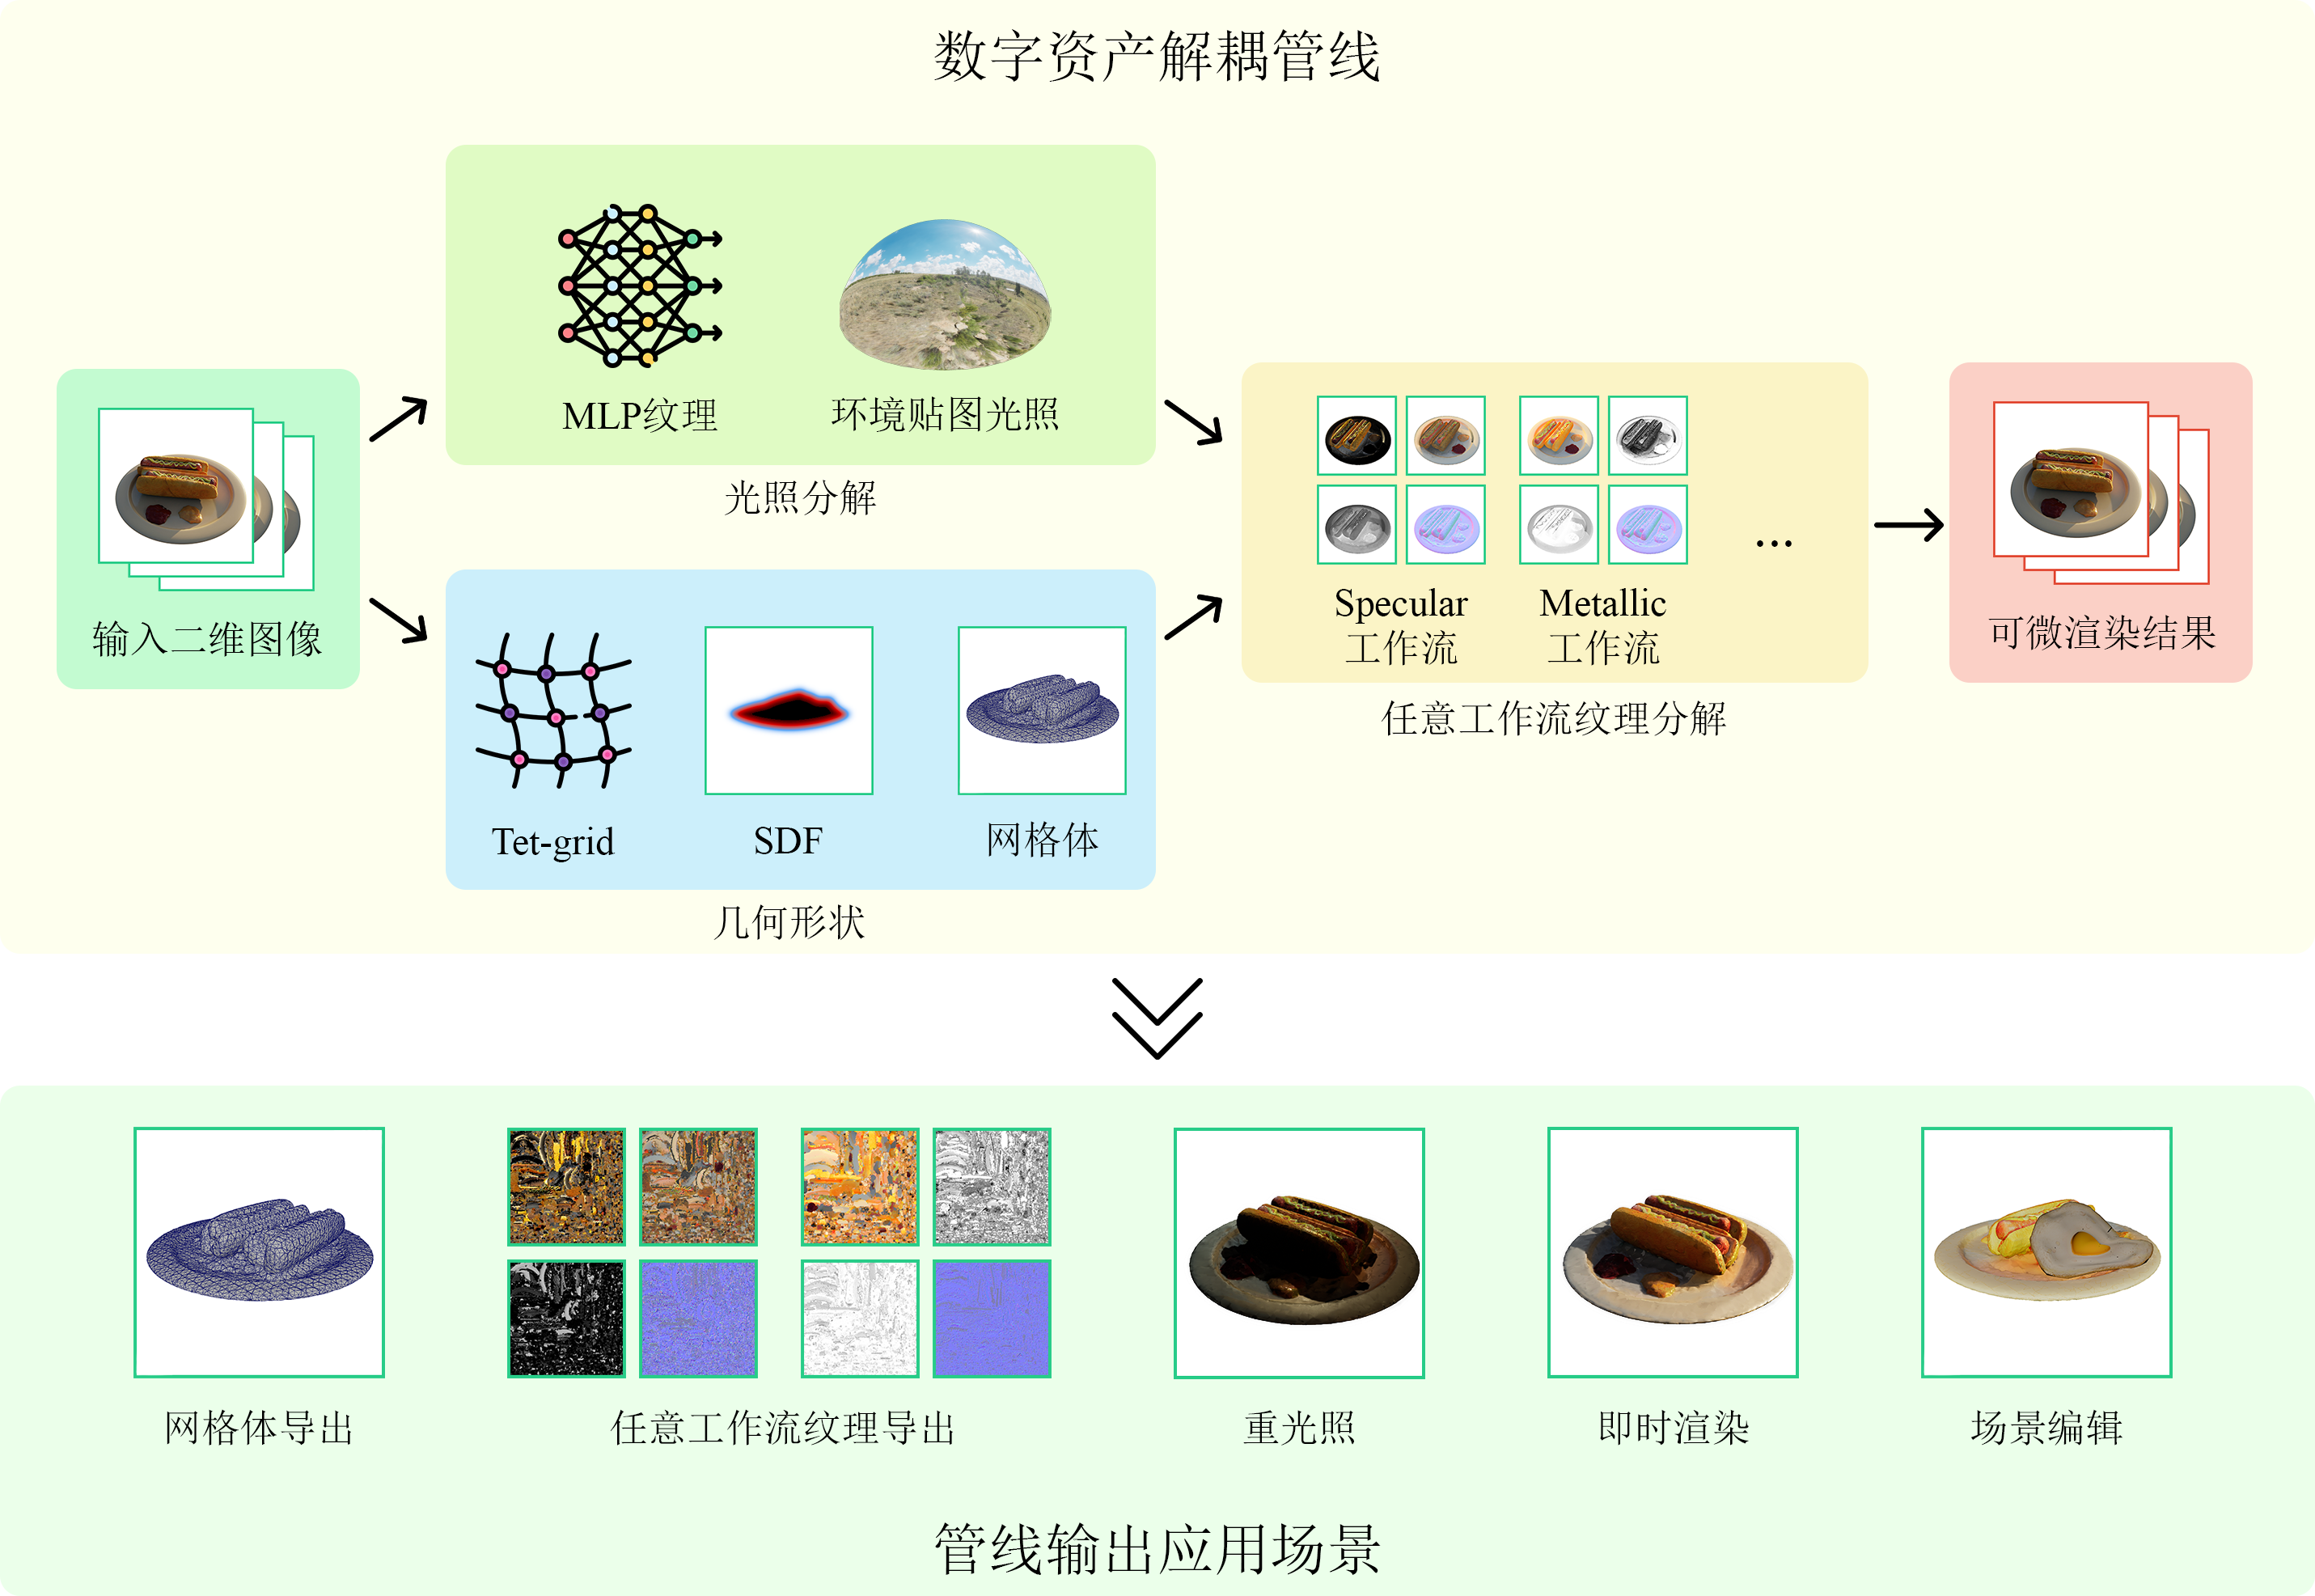
\includegraphics[width=1.0\linewidth]{Main_line_with_apply_with_big_zi.png}
  \caption{数字资产解耦管线与应用场景}
  \label{fig:main_pipe_line}
\end{figure}

\section{数字资产解耦问题分析}

工业界现有的资产大多归属于特定的工作流,而不同的着色模型也与工作流逐一对应,因此,
本文管线如果能够实现将任意工作流的数字资产转换到另一种任意工作流,即可将数字资产与任意的渲染技术相结合,
实现本文解耦的目标。

在技术路线上,本文选择了第二章中介绍的NeRF光照分解相关研究,在此基础上进行目标的实现。
NeRF光照分解管线所需的输入为场景的二维RGB图片,而待转换的数字资产可以通过渲染获得这些图片;
同时,该管线可以输出场景的几何形状和表面反射属性,与数字资产转换所需的输出类似。因此,
选择该技术开展研究和实现,对于本文的目标具备可行性。

但是,现有的工作为了提升几何重建效果,大多延续了NeRF中的隐式神经几何表示,
这导致管线的输出仅能用于重光照或新视角合成任务。而本文的目标是管线的输出能够无缝对接传统渲染器,
应用于即时渲染和下游编辑,因此本文需要对管线中的几何表示进行改造,使其输出显式网格体几何表示。
其次,现有管线受限于可微渲染的优化效率,多采用数据驱动的BRDF或固定规格的参数化BRDF作为反射属性表示,
无法满足本文使用任意工作流的需求,所以有必要针对反射属性部分重新设计,把指定工作流的纹理贴图作为输出。

基于以上分析,本文将目标进一步设置为,设计并实现一套管线,其输入为多张相机位姿已知、
光照环境及场景三维信息未知的二维RGB图片;输出为场景的几何形状和反射属性。其中,
输出的几何表示为网格体,反射属性为指定工作流对应的纹理贴图。

\section{管线设计}
本节将系统地介绍本文管线的设计与创新方法。首先,本文改进了几何表示方式,
通过一种显式隐式混合的方法,使得管线能够基于隐式表示进行优化的同时,
也能够直接输出显式网格表示的场景几何信息。随后,本文采用MLP纹理表示场景的表面反射属性,
这种设计带来了足够的灵活性,能够满足本文对任意工作流进行解耦的需求。
结合环境光照贴图作为光照技术进行可微渲染。在可微渲染中,本文允许使用任意的工作流表示
作为场景的反射属性的表示方法,使用渲染结果与原始输入计算损失,并将梯度传播到前述的几个阶段。
最后,本文管线输出网格体与纹理贴图,完成数字资产解耦的目标。接下来,本节将分别介绍以上部分。

\subsection{几何表示方式}

现有的隐式神经表示方法难以将生成结果直接用于下游编辑等任务,而传统的显式网格体则在重建效果上有所折损。
因此,本文采用了混合的几何表示方法DMTet\cite{shen2021deep},
其结合了SDF与网格体表示的优点,同时能够与传统渲染器无缝衔接。

根据\ref{sec:geo_representation}的介绍,DMTet能够先通过SDF学习几何形状,随后以可微的方式转换为三角面网格体。
为了更高效地利用这种混合形状表示,本文进一步拓展了DMTet,引入了即时渲染中法线纹理这一技术,
在优化过程中依次使用SDF、网格体、法线纹理进行优化,接下来本文将详细介绍设计思路及实现方式。

在传统的渲染管线中,网格体在细节的精细程度取决于两个方面,首先是网格体的顶点数量,
对于细节较为丰富的区域,较高的顶点数量才能准确的还原精细结构;其次是网格体的拓扑结构,
其决定着顶点的连接和排布方式,理想的拓扑结构可以将顶点和边分配在形状发生突变的位置,
以实现相同的几何形状的同时使用尽可能少的顶点。所以,传统的数字资产在制作时通常会先完成一个较为精细的“高模”,
然后制作一个多边形数量较低的“低模”。在这一过程中,艺术家根据经验设置网格的拓扑结构,最后通过烘焙(Baking)
将“高模”中的细节以法线纹理的形式转移至“低模”中,如图\ref{fig:baking_normal}所示。
\begin{figure}[H]
  \centering
  % 这里可以控制图片宽度比例
  \begin{subfigure}[t]{0.24\textwidth}
    \centering
    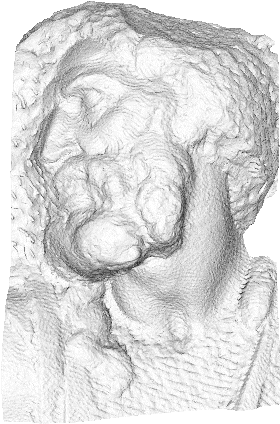
\includegraphics[height=4cm]{ch3/normal_baking/ori.png}
    \caption{高模}
  \end{subfigure}
  \begin{subfigure}[t]{0.24\textwidth}
    \centering
    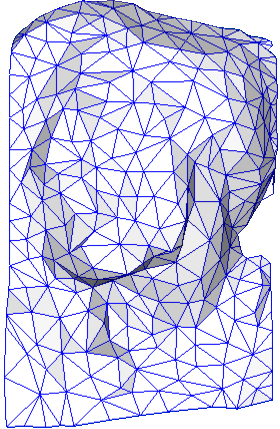
\includegraphics[height=4cm]{ch3/normal_baking/low_poly.png}
    \caption{低模}
  \end{subfigure}
  \begin{subfigure}[t]{0.24\textwidth}
    \centering
    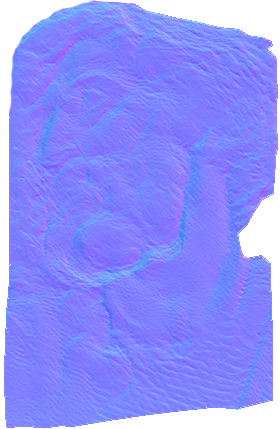
\includegraphics[height=4cm]{ch3/normal_baking/normal.png}
    \caption{法线纹理}
  \end{subfigure}
  \begin{subfigure}[t]{0.24\textwidth}
    \centering
    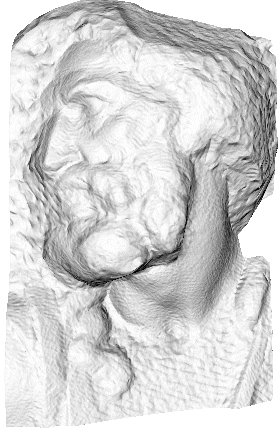
\includegraphics[height=4cm]{ch3/normal_baking/mapped.png}
    \caption{使用法线纹理}
  \end{subfigure}
  \caption{烘焙过程示意}
  \label{fig:baking_normal}
\end{figure}
基于以上这一流程,本文引入了类似烘焙的过程来提升几何估计的准确度,从而改善3D几何形状重建的质量。
本文设计的管线中将依次对SDF、网格体、法线纹理进行优化。首先,
SDF作为一种精细但计算效率较低的表示方式,视为“高模”,该阶段的优化目标是,发挥SDF在高频细节表示上的优势,
尽可能还原场景中的所有细节,以确保下一阶段中使用的网格具有足够的几何细节和拓扑结构。
随后,网格体的拓扑结构在经过初步的优化后将被固定,这一阶段的几何表示视为“低模”,
该优化阶段不断调整网格的顶点位置,使其精确包裹住场景的真实形状。最后,在网格体的形状确定后,
法线纹理的优化将用于表达细微的几何细节,以将场景的高频细节传递至最终网格模型中。

按照上文的设计及前期实验结果,本文针对性地设计了不同的正则项和权重,分阶段引导管线完成上述过程,具体的损失函数和策略如下:

\fourthtitle{1}法线平滑正则项

当模型尝试恢复几何形状时,法线纹理的引入会增加形状的不确定性。比如,某个突起的几何结构既可能是来自于法线纹理,
也可能来自于网格体。如果模型依赖于法线纹理进行重建,可能会导致“低模”形状无法得到有效还原,折损后续重建效果。
因此,本文选择使用损失函数限制法线纹理的变化,使网格体在初始化阶段保持法线纹理相对平滑,
尽可能地通过网格体形状表示场景细节。该损失函数可以由以下公式表示:
本文将平滑正则项应用于法线纹理,以惩罚网络过早地将几何细节表示为法线纹理的行为。该正则项$\mathcal{L}_{\text{nrm}}$
可以被表示为:
\begin{equation}
  \label{eq:nrm_smooth}
  \mathcal{L}_{\text{nrm}} = \sum_{\mathbf{x_\text{surf}}} {\lvert {n({\mathbf{x_\text{surf}}})} - {n({\mathbf{x_\text{surf}}}+\epsilon)}\rvert}
\end{equation}
其中,$\mathbf{x_\text{surf}}$为表面着色点的位置,$\epsilon$为随机的位移。通过类似于抖动的采样方式,计算法线纹理
不同区域的变化程度,并强制网络使用更为平滑的纹理。该损失项的权重随训练步数而逐渐降低,允许网络在网格体细节初步建立之后,
再使用法线纹理加入更多细节。

\fourthtitle{2}拉普拉斯正则项

在初期的实验结果中,DMTet生成的网格体通常会将多个顶点挤压在一起,以形成尖锐结构或小块平坦表面。
在可微渲染管线中,这种重叠顶点不会产生严重的渲染错误,但在传统渲染器中会导致渲染出伪影。在总体形状的表达上,
重叠顶点也会导致大量的顶点和面被浪费,折损几何重建效果。因此,本文利用均匀拉普拉斯矩阵(Uniform Laplacian)
计算正则项,引导网络将顶点分散开。均匀拉普拉斯矩阵$\symbfit{L}$基于顶点邻接关系计算:
\begin{equation}
  \symbfit{L}_{ij} =
  \begin{cases}
  -1, & \text{if } i \text{ and } j \text{ are adjacent} \\
  d_i, & \text{if } i = j \\
  0, & \text{otherwise}
  \end{cases}
  \label{eq:uniform_lap}
\end{equation}
其中,$d_i$代表顶点的度数,即它的邻接顶点个数。拉普拉斯正则项$\mathcal{L}_\text{lap}$计算方式如算法\ref{alg:lapreg}所示:
\renewcommand{\algorithmicrequire}{\textbf{输入:}\unskip}
\renewcommand{\algorithmicensure}{\textbf{输出:}\unskip}
\begin{algorithm}
  \caption{拉普拉斯正则化损失计算}
  \begin{algorithmic}[1]
  \REQUIRE 顶点坐标矩阵$\mathbf{V} \in \mathbb{R}^{V \times D}$, 三角面矩阵$\mathbf{F} \in \mathbb{N}^{F \times 3}$
  \ENSURE 拉普拉斯正则项 $\mathcal{L}_{\text{lap}}$
  \STATE Initialize sparse matrix $L \in \mathbb{R}^{V \times V}$ with zeros
  \FOR{each face $f = (i, j, k) \in \mathbf{F}$}
      \STATE Add edges $(i, j), (j, k), (k, i)$ to adjacency list
  \ENDFOR
  \FOR{each edge $(i, j)$ in adjacency list}
      \STATE $L_{ij} \gets -1$, $L_{ji} \gets -1$
  \ENDFOR
  \FOR{each vertex $i$}
      \STATE $L_{ii} \gets -\sum_{j \neq i} L_{ij}$
  \ENDFOR

  \STATE Compute $\delta \gets L \mathbf{V}$
  \STATE Compute $\|\delta_i\| = \sqrt{\sum_{d} \delta_{i,d}^2}$ for each vertex $i$
  \STATE Compute $\mathcal{L}_{\text{lap}} \gets \frac{1}{V} \sum_{i=1}^{V} \|\delta_i\|$
  \STATE \RETURN $\mathcal{L}_{\text{lap}}$
  \end{algorithmic}
  \label{alg:lapreg}
\end{algorithm}

\fourthtitle{3}SDF翻转正则项

由于SDF转换为网格体时不可避免地产生翻转或浮动的三角形面,因此本文采用了Liao等人\cite{Liao_2018}
提出的方法对DMTet的SDF值进行正则化。给定二元交叉熵损失函数$H$、Sigmoid函数$\sigma$和
符号函数$\mathrm{sign}(s_i)$,在满足$\mathrm{sign}(s_i)\neq\mathrm{sign}(s_j)$的条件下,
正则化项可以通过以下公式定义:
\begin{equation}\label{eq:Lreg}
L_{reg}=\sum_{i,j\in\mathbb{S}_e}\Bigl[H\bigl(\sigma(s_i),\mathrm{sign}(s_j)\bigr)+H\bigl(\sigma(s_j),\mathrm{sign}(s_i)\bigr)\Bigr]
\end{equation}
其中,$\mathbb{S}_e$表示四面体网格中边的集合,且条件为$\mathrm{sign}(s_i)\neq\mathrm{sign}(s_j)$。
该正则化项的直观解释是减少符号翻转的次数,从而简化表面,避免不必要的浮动几何体或内部几何结构。

\subsection{MLP纹理} \label{sec:mlp_texture}
由于本文旨在使用任意工作流所对应的标准进行NeRF光照分解,因此有必要设计一种足够灵活、
易于拓展的实现方式。本文使用MLP来估计表面反射属性,以类似于体积纹理的方式建立不同的属性,
并按照通道重新划分输出用于后续的渲染步骤。

MLP整体结构如图\ref{fig:mlp_texture_cn}所示。模型首先对输入的三维坐标进行归一化处理,并利用tiny-cuda-nn框架\cite{Muller_tiny-cuda-nn_2021}
中提供的哈希网格编码器对其进行多分辨率特征映射,将输入坐标映射到高维特征空间中,增强网络对细粒度纹理信息的捕捉能力。
随后,编码器输出的特征将作为MLP的输入。MLP由一个初始全连接层,若干使用ReLU激活函数的隐藏层,以及一个输出层组成。
\begin{figure}[htb]
  \centering
  % 这里可以控制图片宽度比例
  
\includegraphics[width=1.0\linewidth]{MLP_texture_cn.png}
  \caption{纹理表示方式}
  \label{fig:mlp_texture_cn}
\end{figure}

由于该MLP表示的是体积纹理,因此还需要额外的采样步骤。本文首先使用xatlas生成网格体的uv坐标,随后在空间中进行采样。
在纹理导出之前,本文额外使用边缘填充算法解决了纹理的接缝问题。边缘填充算法的计算过程为算法\ref{alg:fillholes}所示:

\renewcommand{\algorithmicrequire}{\textbf{输入:}\unskip}
\renewcommand{\algorithmicensure}{\textbf{输出:}\unskip}

\begin{algorithm}
  \caption{填充空洞推拉算法}
  \label{alg:fillholes}
  \small
  \begin{algorithmic}[1]
  \REQUIRE 源图像 \texttt{src}
  \ENSURE 目标图像 \texttt{dst}
  
  \STATE 初始化图像金字塔容器 \texttt{pyramid}
  
  \STATE 创建与\texttt{src}同规格的浮点格式图像 \texttt{top}
  \STATE 将\texttt{src}拷贝至\texttt{top}
  \STATE 添加\texttt{top}到\texttt{pyramid}
  
  \WHILE{当前层宽或高 > 1}
      \STATE 获取当前层图像\texttt{big}
      \STATE $\texttt{w} \gets \max(1, \lfloor \texttt{w}/2 \rfloor)$,$\texttt{h} \gets \max(1, \lfloor \texttt{h}/2 \rfloor)$
      \STATE 创建缩小尺寸的图像 \texttt{small}
      \STATE 将\texttt{big}下采样到 \texttt{small}
      \STATE 对\texttt{small}的非零 $\alpha$ 像素执行:$\texttt{RGB} \gets \texttt{RGB} / \alpha$
      \STATE 添加\texttt{small}到\texttt{pyramid}
  \ENDWHILE
  \STATE $i \gets |pyramid| - 2$
  \WHILE{$i \textgreater 0$}
      \STATE 获取当前层图像\texttt{big}
      \STATE 创建\texttt{blowup}图像,规格与\texttt{big}相同
      \STATE 将下一层图像上采样到\texttt{blowup}
      \STATE 将\texttt{big}与\texttt{blowup}进行 $\alpha$ 合成:$\texttt{big} \gets \texttt{over}(\texttt{big}, \texttt{blowup})$
      \STATE $i \gets i - 1$
  \ENDWHILE

  \RETURN pyramid[0]
  \end{algorithmic}
  \end{algorithm}

最周,本文参照NeRFactor\cite{zhang2021nerfactor},使用与\ref{eq:nrm_smooth}相似的损失函数,对不同的纹理进行平滑。

\subsection{光照表示}
本文使用第2章中介绍的IBL技术作为光照表示技术。根据\eqref{eq:rendering_equation}中的渲染方程,物体表面的出射光照
可以表示为:
\begin{equation}
  \label{eq:radiance}
  L\left(\omega_o\right)=\int_{\upOmega} L_i\left(\omega_i\right)f\left(\omega_i,\omega_o\right)\left(\omega_i\cdot\mathbf{n}\right)\mathrm{d}\omega_i,
\end{equation}
其中$L_i$表示来自方向$\omega_i$的入射辐射,$f\left(\omega_i,\omega_o\right)$为BRDF,积分域$\upOmega$为以
表面法线$\mathbf{n}$为中心的半球。由于完整的光照计算开销较高,本文使用了传统渲染引擎中常见的近似方法\cite{Hill_2014},
使用分裂和近似以进一步减少计算量。

\section{实验与结果分析}
通过前两节的分析与介绍,本文设计并实现了数字资产解耦管线,该管线能够按照任意工作流进行光照分解。为了验证
本文方法及管线的适用性和有效性,本文进行了全面的实验。接下来,本文将先介绍所用的数据集,随后进行定量实验以及定性实验,
并对实验结果进行分析。
\subsection{数据集}

为了验证本文提出的NeRF光照分解管线的有效性,我们使用公开可获取的NeRF合成数据集进行实验。
NeRF合成数据集是一个广泛使用的基准数据集,具有丰富的合成场景和高质量的图像数据,
能够充分证明本文方法在不同场景下的泛化能力。其特点包括多种复杂的场景几何形状、
不同的光照条件以及多视角的观察角度,是理想的实验数据。

其中,本文选择了4个场景,作为可视化的定性实验,随后在完整数据集上进行定量实验。
本文选择的可视化场景及理由如下:

\fourthtitle{1} Lego:
该场景包含一台由多种不同形态和颜色的积木组成的挖掘机,具有复杂的几何结构和显著的表面光泽,
可以充分验证本文管线对高频几何细节的还原能力。

\fourthtitle{2} Hotdog:
这个场景包含圆润的食物和餐具,同时具有多样的高光反射特性,对本文管线分解光泽表面的能力提出了挑战。

\fourthtitle{3} Materials:
该场景呈现了多种不同的材料,如镜面金属、磨砂金属等,每种材料具有不同的光反射属性,
能够满足验证管线识别金属或高光区域并分解的能力。

\fourthtitle{4} Mic:
该场景包括了一些微小的物体和细节,如精细结构的物体表面,并且主体材质多为磨砂金属,
可以用来验证管线在高精度要求下的适用性。

以上四个场景的预览如图\ref{fig:exp_scene}所示。

\begin{figure}[H]
  \centering
  % 这里可以控制图片宽度比例
  \begin{subfigure}[t]{0.24\textwidth}
    \centering
    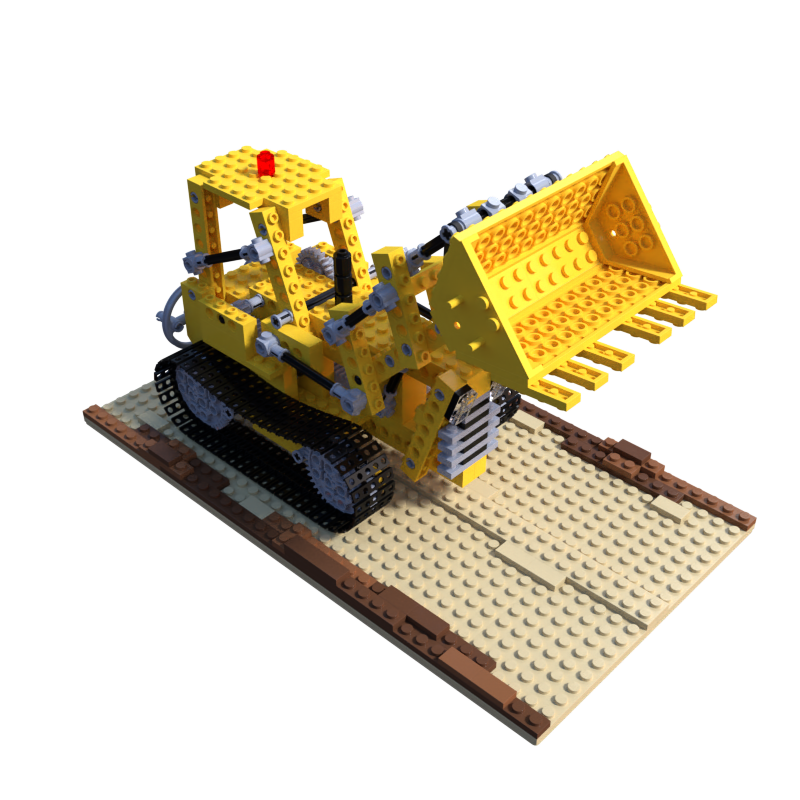
\includegraphics[width=\linewidth]{ch3/exp_scene/lego.png}
    \caption{Lego}
  \end{subfigure}
  \begin{subfigure}[t]{0.24\textwidth}
    \centering
    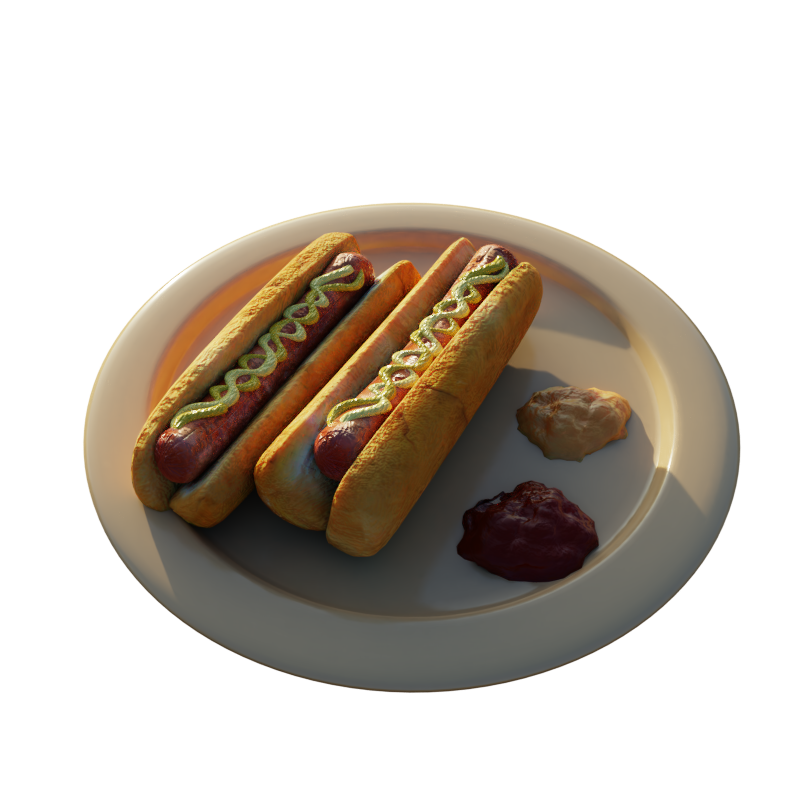
\includegraphics[width=\linewidth]{ch3/exp_scene/hotdog.png}
    \caption{Hotdog}
  \end{subfigure}
  \begin{subfigure}[t]{0.24\textwidth}
    \centering
    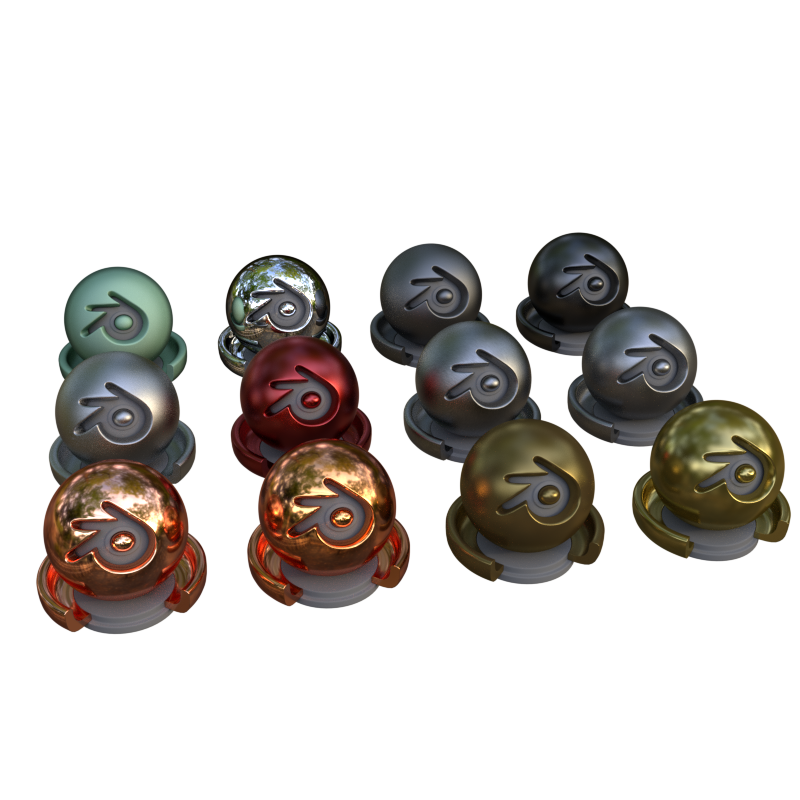
\includegraphics[width=\linewidth]{ch3/exp_scene/materials.png}
    \caption{Materials}
  \end{subfigure}
  \begin{subfigure}[t]{0.24\textwidth}
    \centering
    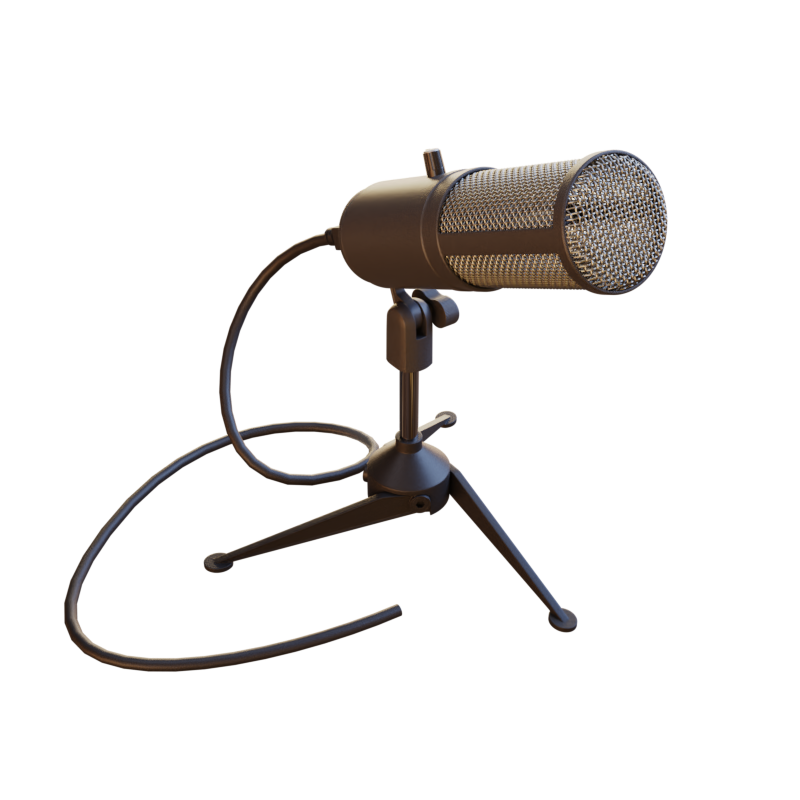
\includegraphics[width=\linewidth]{ch3/exp_scene/mic.png}
    \caption{Mic}
  \end{subfigure}
  \caption{实验场景预览}
  \label{fig:exp_scene}
\end{figure}

\subsection{多种工作流分解效果实验}
本节展示了本文提出的NeRF光照分解管线在处理任意工作流资产时的解耦效果。
在2.2.3中,我们详细介绍了3种不同的工作流,分别是Metallic工作流、Specular工作流
以及Blinn-Phong工作流。这些工作流至今仍在传统渲染引擎中得到广泛应用,
本节实验将基于这三种工作流进行分解,并展示其中4个具有代表性的不同场景可视化展示,
以定性证明本文管线能够对多种工作流进行分解。随后,本文对数据集中的全部场景进行定量比较,
分析了不同工作流对分解效果的影响。

\begin{figure}[htbp]
  \centering
  \renewcommand{\arraystretch}{1} % 调整表格行距
  \setlength{\tabcolsep}{3pt} % 调整列间距

  \begin{tabular}{c c c c c} 
      & Lego & Hotdog & Materials & Mic\\

      \raisebox{2.5\height}{\rotatebox[origin=c]{90}{Albedo}} & % 关键修改
      \subfloat{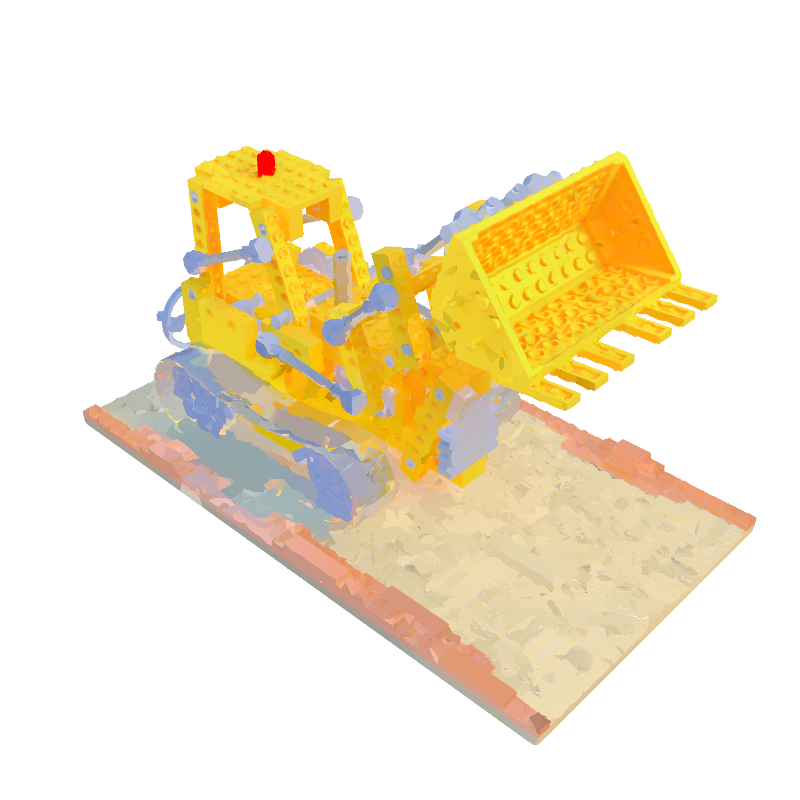
\includegraphics[width=0.22\textwidth]{ch3/metallic_show/lego/kd.png}} &
      \subfloat{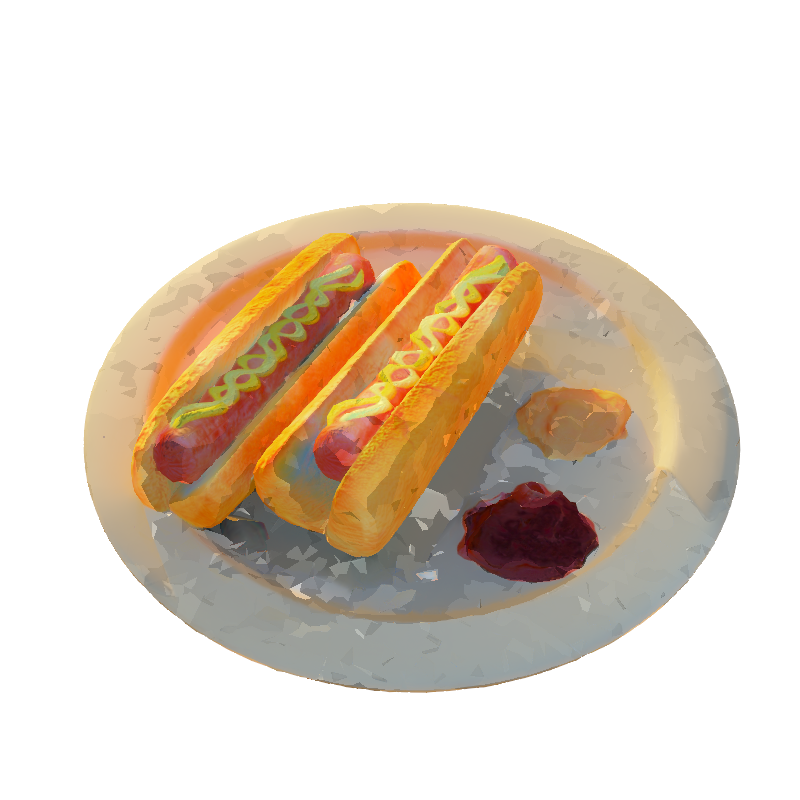
\includegraphics[width=0.22\textwidth]{ch3/metallic_show/hotdog/kd.png}} &
      \subfloat{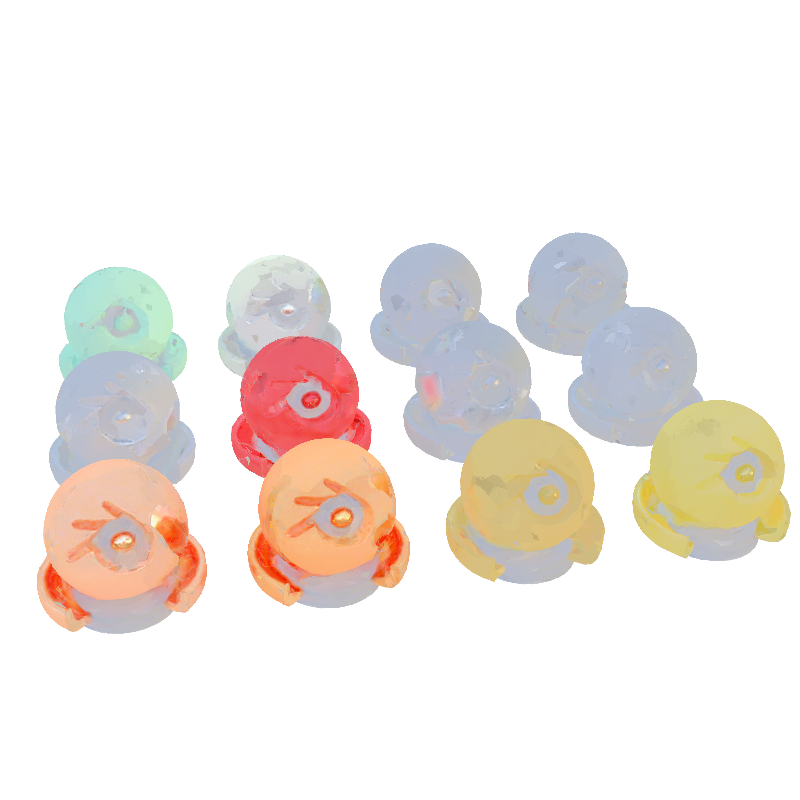
\includegraphics[width=0.22\textwidth]{ch3/metallic_show/materials/kd.png}} &
      \subfloat{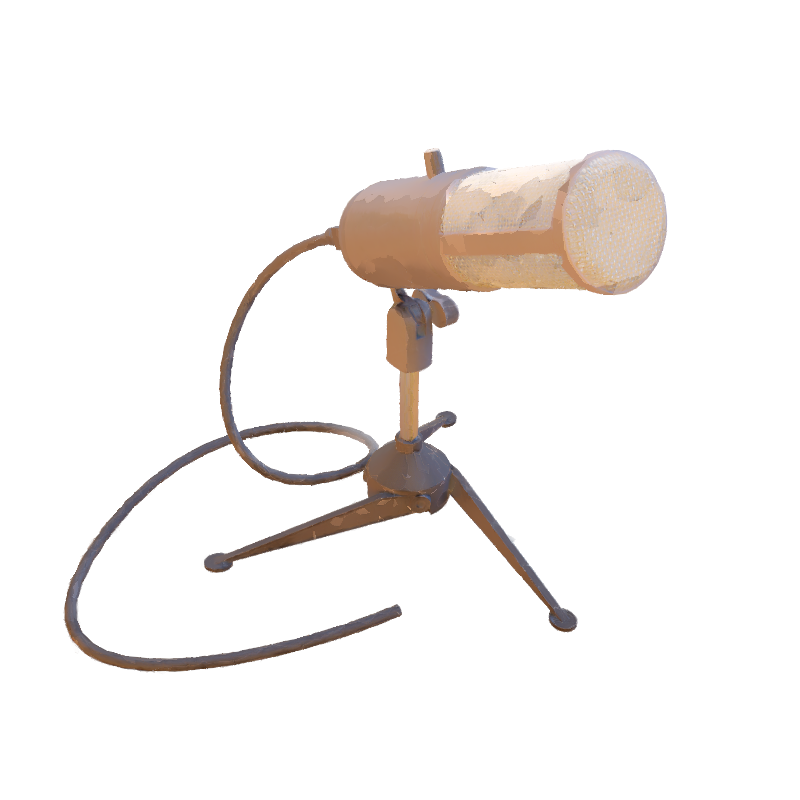
\includegraphics[width=0.22\textwidth]{ch3/metallic_show/mic/kd.png}} \\

      \raisebox{2\height}{\rotatebox[origin=c]{90}{Metallic}} & % 关键修改
      \subfloat{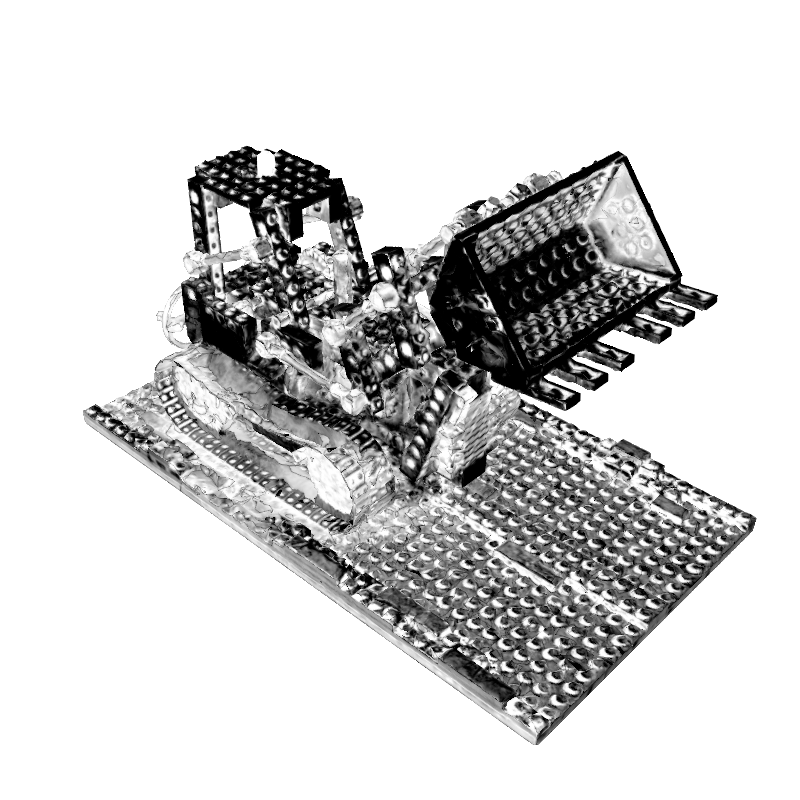
\includegraphics[width=0.22\textwidth]{ch3/metallic_show/lego/m.png}} &
      \subfloat{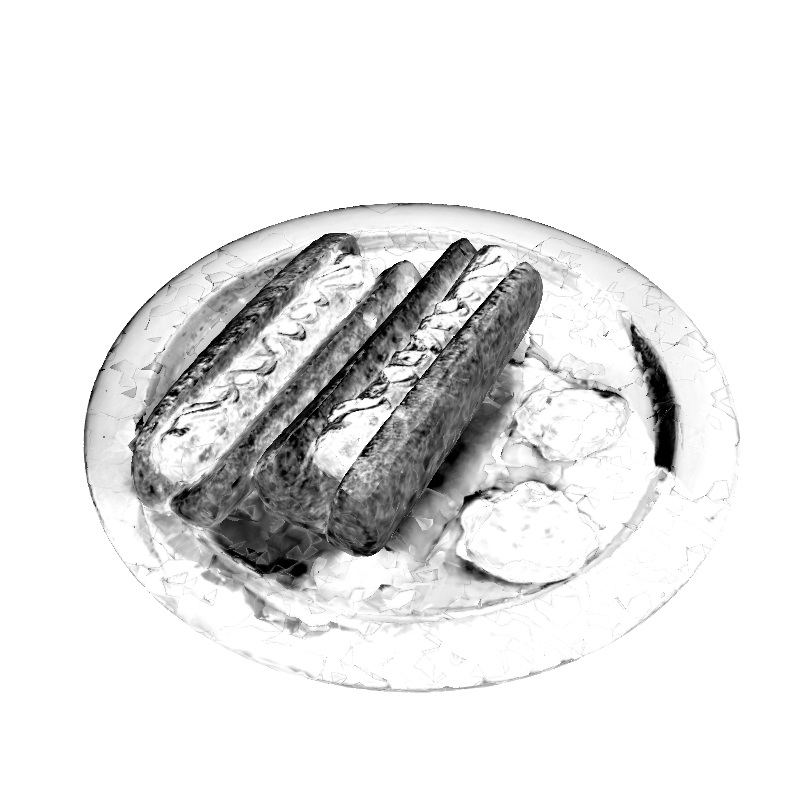
\includegraphics[width=0.22\textwidth]{ch3/metallic_show/hotdog/m.png}} &
      \subfloat{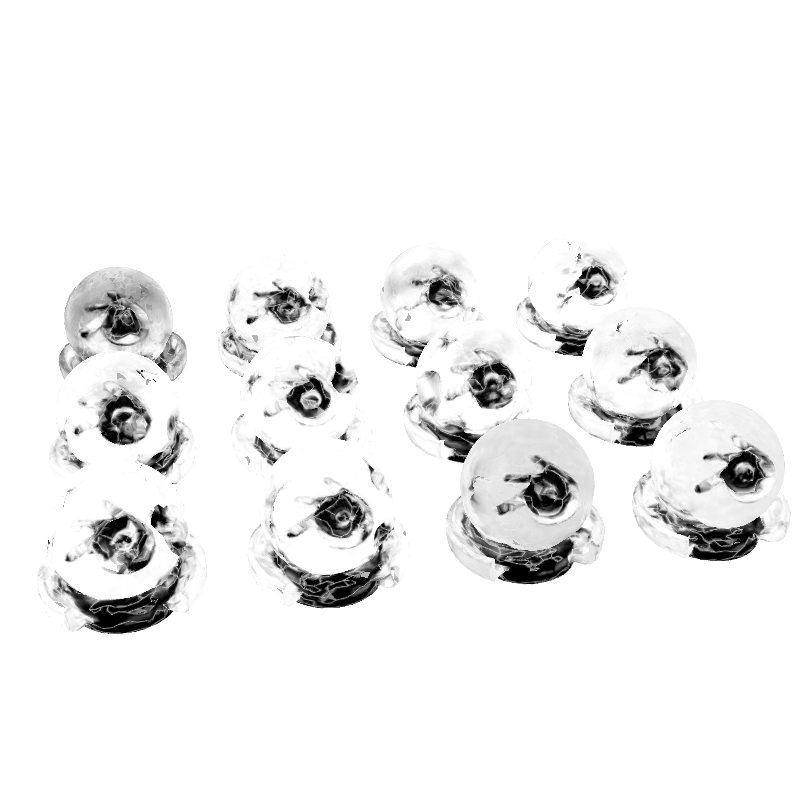
\includegraphics[width=0.22\textwidth]{ch3/metallic_show/materials/m.png}} &
      \subfloat{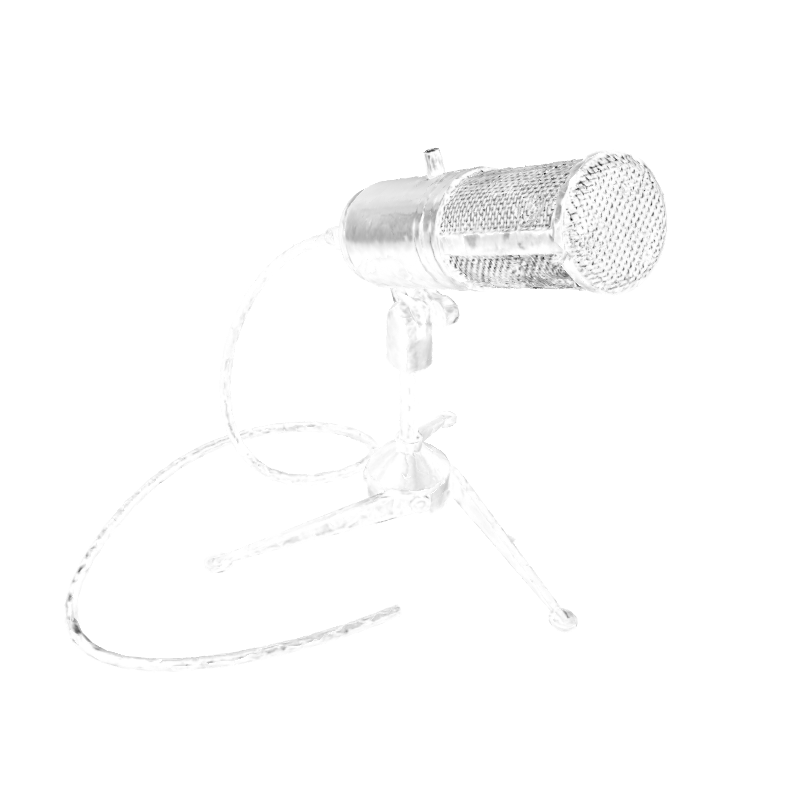
\includegraphics[width=0.22\textwidth]{ch3/metallic_show/mic/m.png}} \\

      \raisebox{1.5\height}{\rotatebox[origin=c]{90}{Roughness}} & % 关键修改
      \subfloat{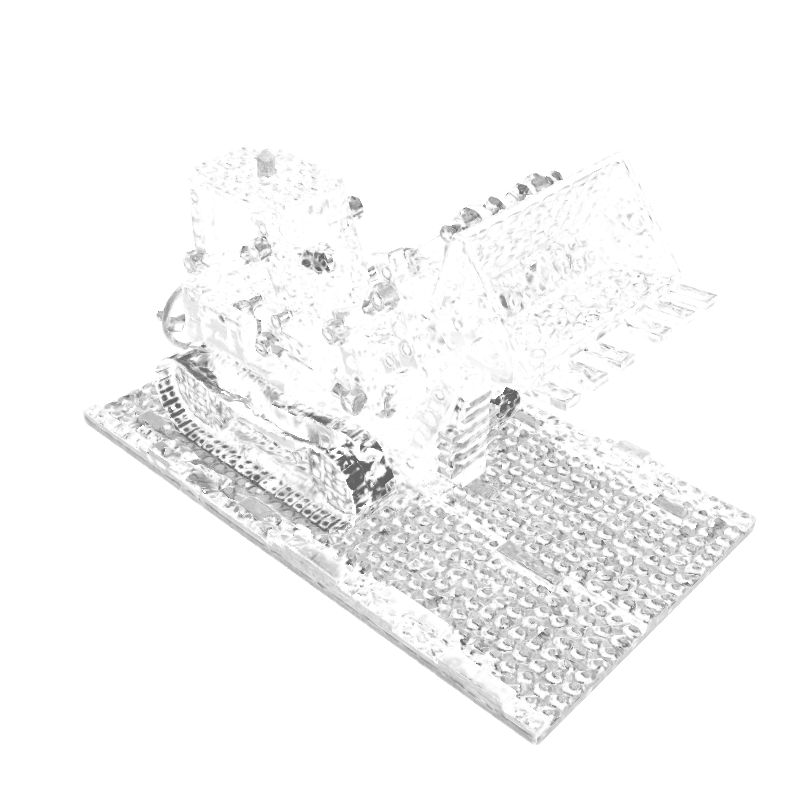
\includegraphics[width=0.22\textwidth]{ch3/metallic_show/lego/r.png}} &
      \subfloat{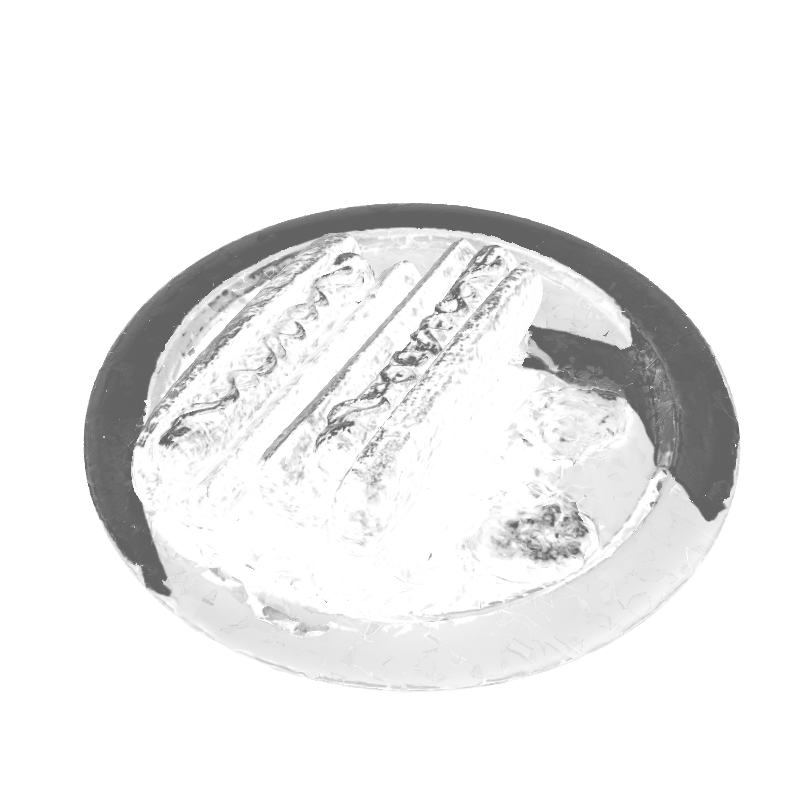
\includegraphics[width=0.22\textwidth]{ch3/metallic_show/hotdog/r.png}} &
      \subfloat{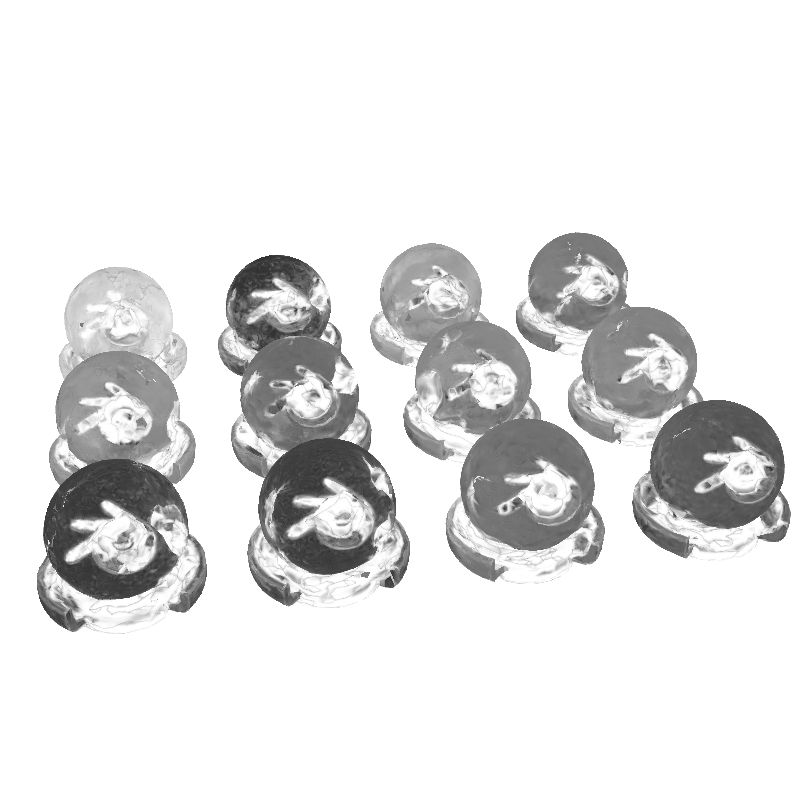
\includegraphics[width=0.22\textwidth]{ch3/metallic_show/materials/r.png}} &
      \subfloat{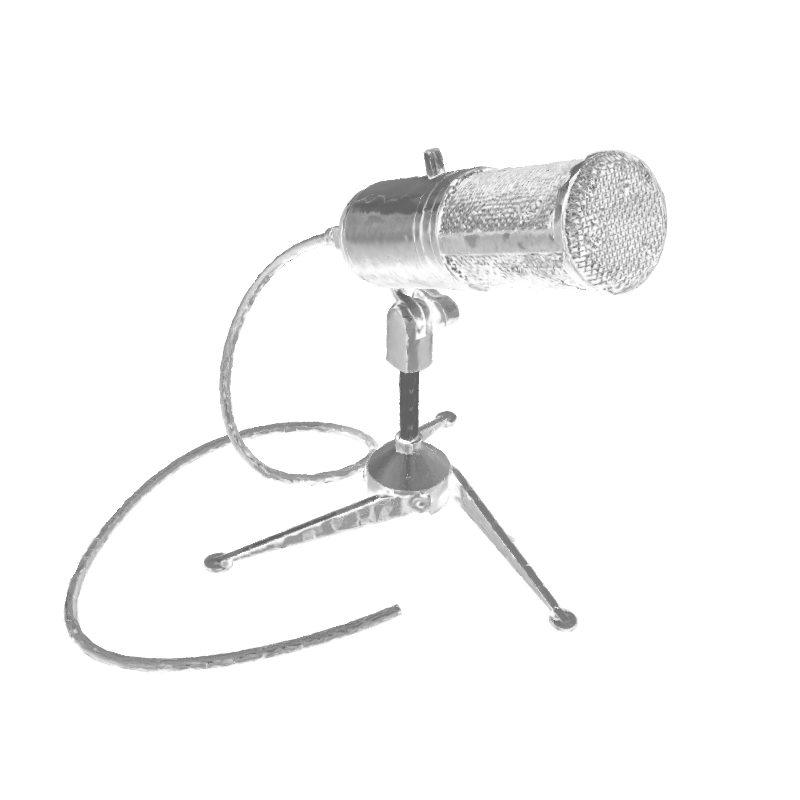
\includegraphics[width=0.22\textwidth]{ch3/metallic_show/mic/r.png}} \\

  \end{tabular}

  \caption{Metallic工作流分解效果}
  \label{fig:metallic_show}
\end{figure}

Metallic工作流分解的实验结果如图\ref{fig:metallic_show}所示,在Metallic工作流下,
管线将输出生成Albedo、Metallic和Roughness三张纹理。在Mic和Materials场景中,
丰富的金属物体使得分解结果的特性尤为显著:Metallic纹理准确标识了金属表面区域,
充分展示了金属材料的高反射性和光泽,证明了该方法在复杂金属表面分解中的适用性。

\clearpage

Specular工作流分解的实验结果如图\ref{fig:specular_show}所示。在Specular工作流下,管线能够同时生成Diffuse、
Specular和Glossiness三张纹理。在Hotdog场景中,光滑的盘子和粗糙的热狗被清晰地区分开来,
漫反射和镜面反射部分清晰可见,证明了该方法在Specular工作流中的适用性。

\begin{figure}[htbp]
  \centering
  \renewcommand{\arraystretch}{1} % 调整表格行距
  \setlength{\tabcolsep}{3pt} % 调整列间距

  \begin{tabular}{c c c c c} 
      & Lego & Hotdog & Materials & Mic\\

      \raisebox{2.5\height}{\rotatebox[origin=c]{90}{Diffuse}} & % 关键修改
      \subfloat{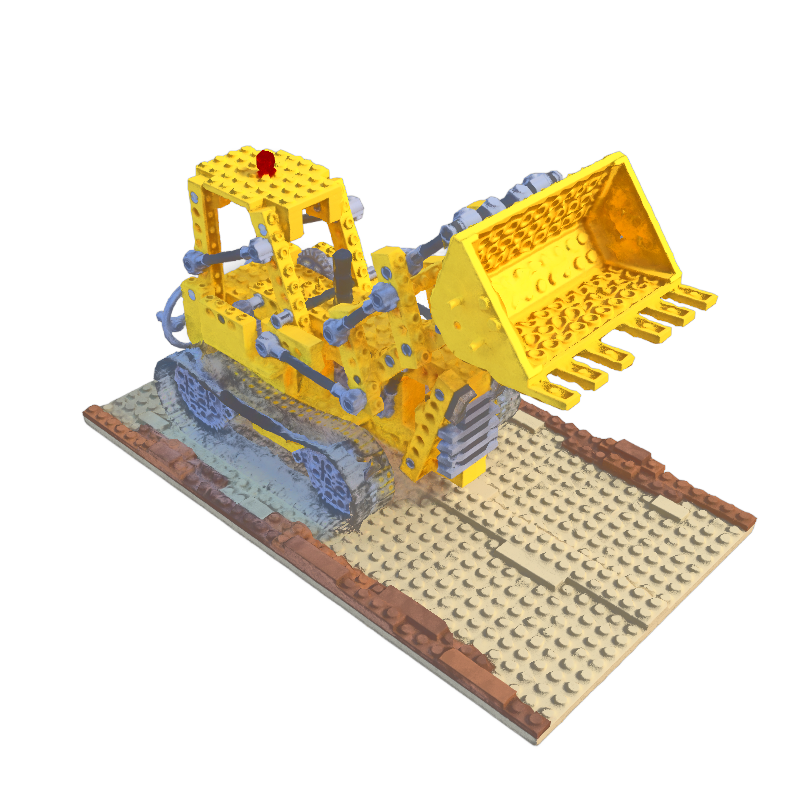
\includegraphics[width=0.22\textwidth]{ch3/specular_show/lego/diff.png}} &
      \subfloat{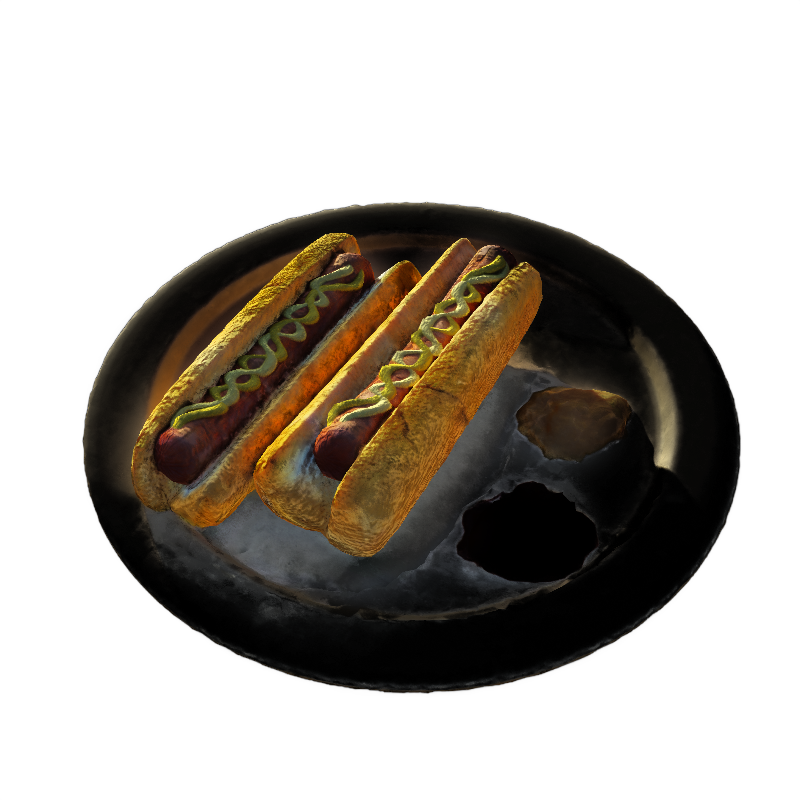
\includegraphics[width=0.22\textwidth]{ch3/specular_show/hotdog/diff.png}} &
      \subfloat{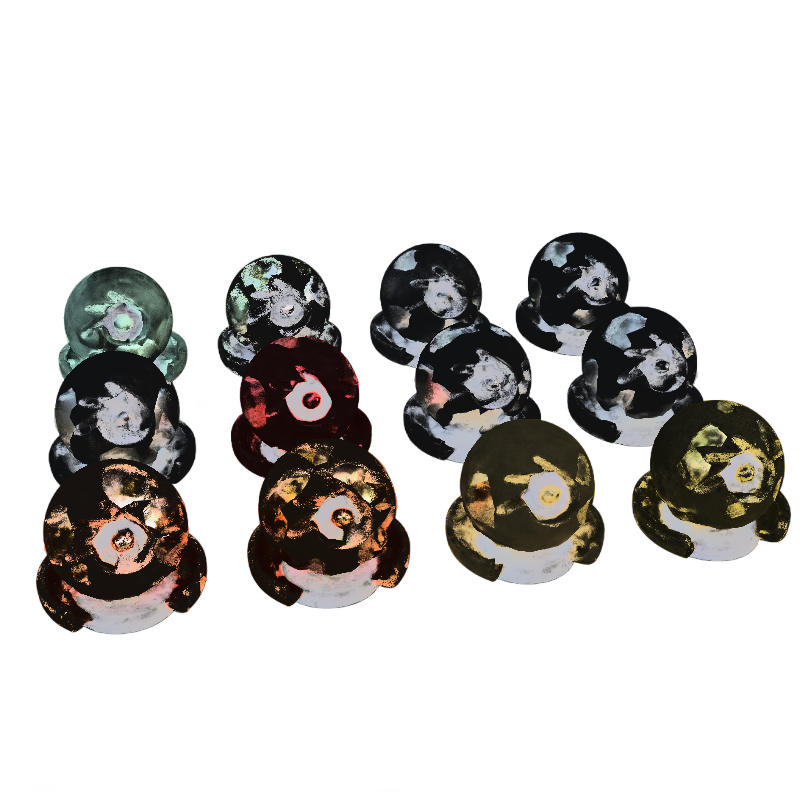
\includegraphics[width=0.22\textwidth]{ch3/specular_show/materials/diff.png}} &
      \subfloat{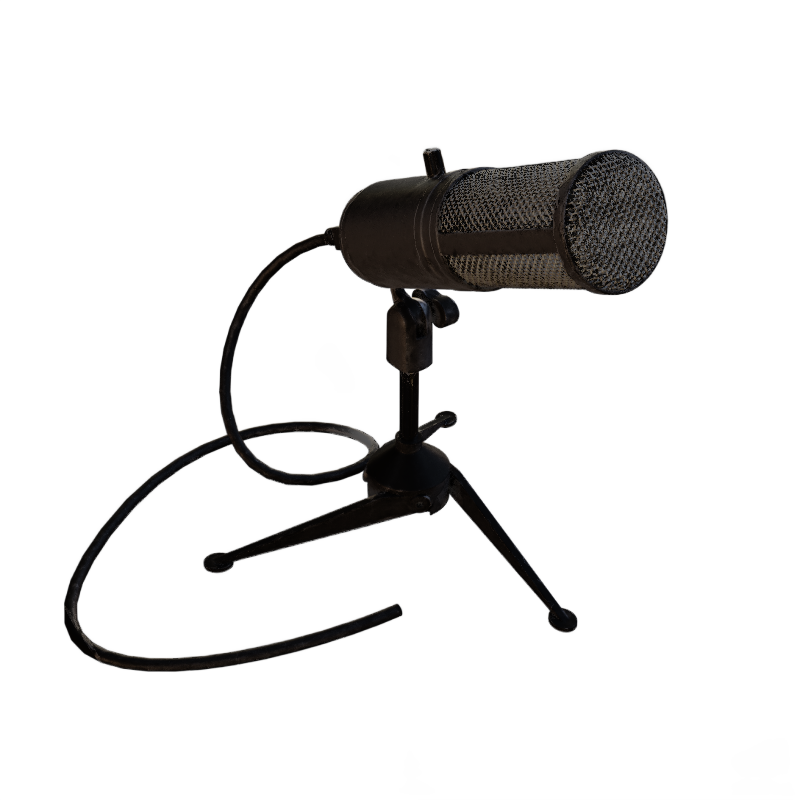
\includegraphics[width=0.22\textwidth]{ch3/specular_show/mic/diff.png}} \\

      \raisebox{2\height}{\rotatebox[origin=c]{90}{Specular}} & % 关键修改
      \subfloat{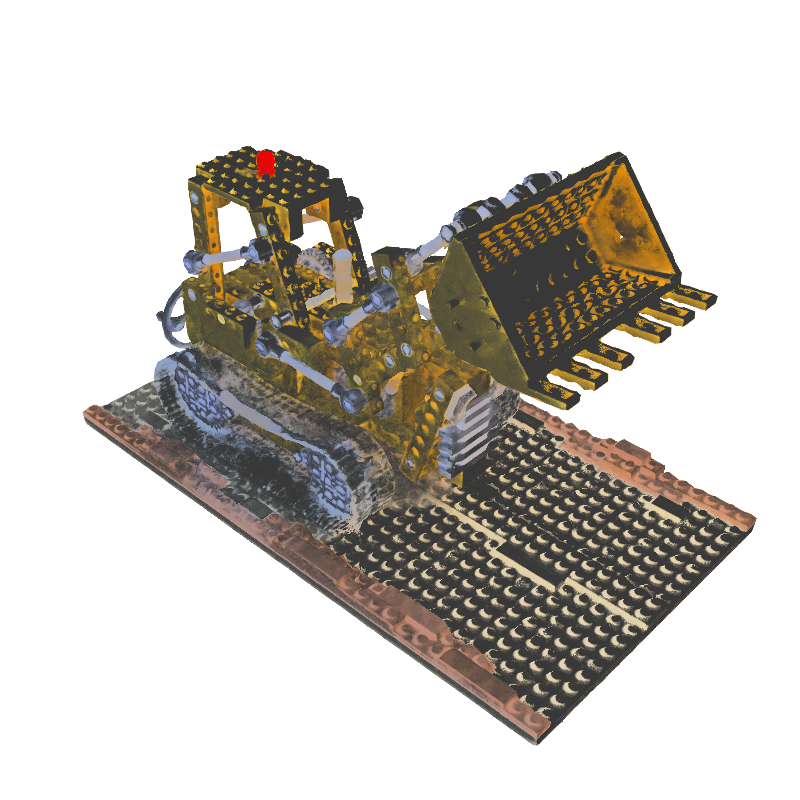
\includegraphics[width=0.22\textwidth]{ch3/specular_show/lego/spec.png}} &
      \subfloat{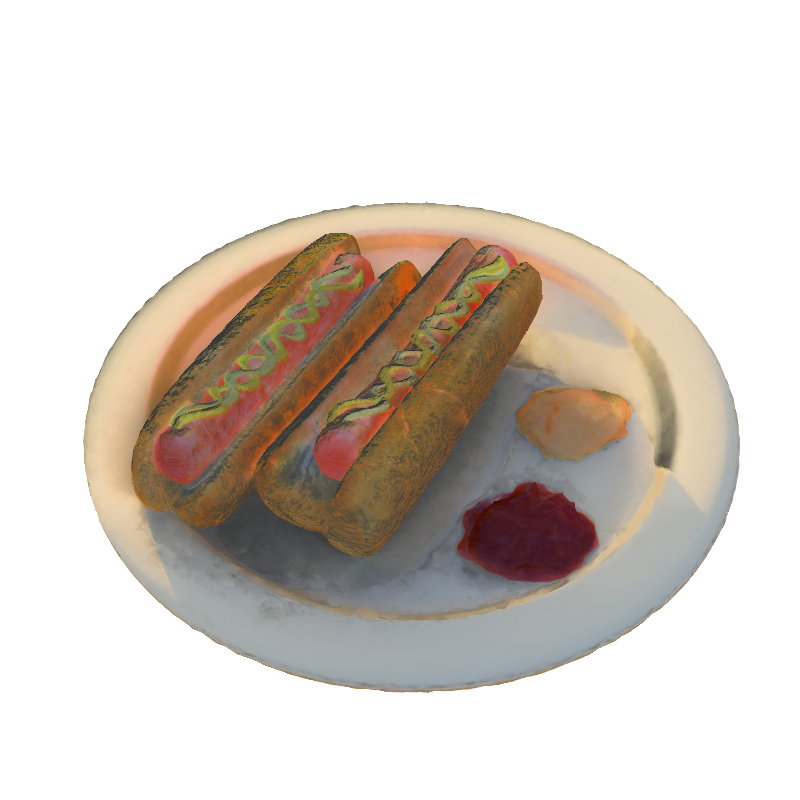
\includegraphics[width=0.22\textwidth]{ch3/specular_show/hotdog/spec.png}} &
      \subfloat{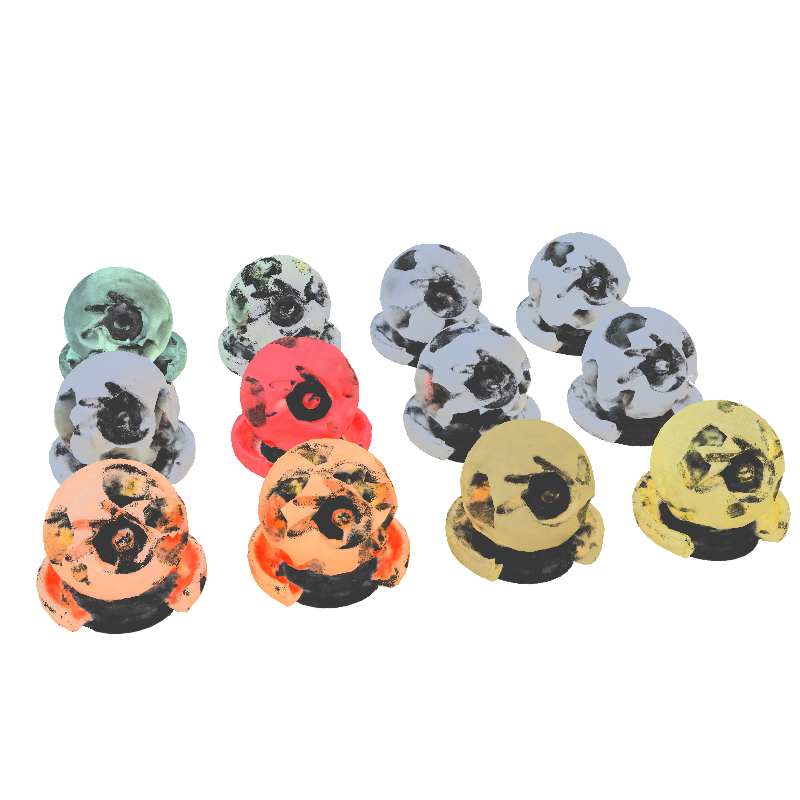
\includegraphics[width=0.22\textwidth]{ch3/specular_show/materials/spec.png}} &
      \subfloat{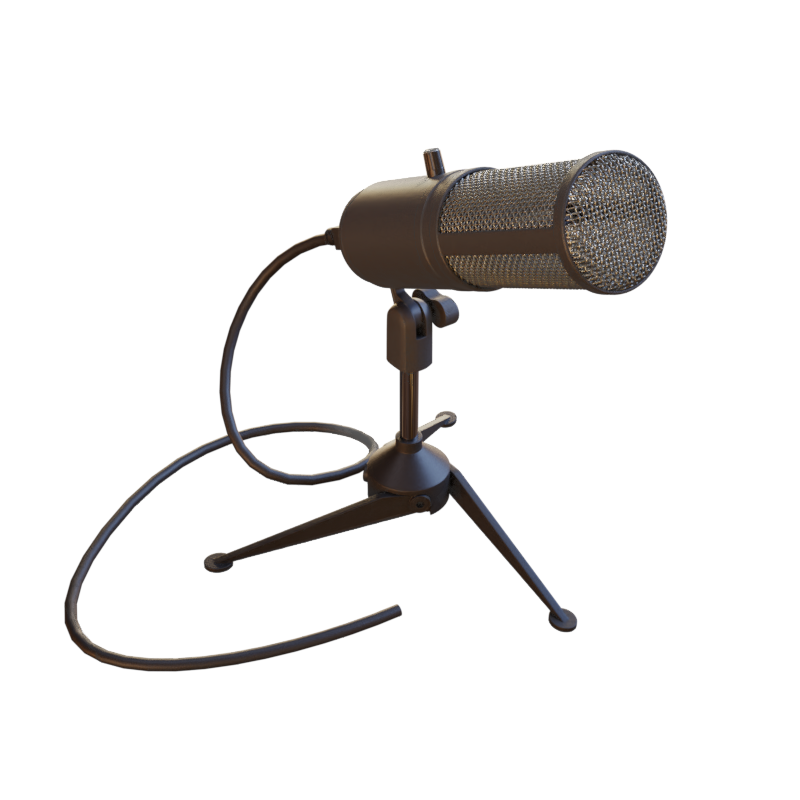
\includegraphics[width=0.22\textwidth]{ch3/specular_show/mic/spec.png}} \\

      \raisebox{1.5\height}{\rotatebox[origin=c]{90}{Glossiness}} & % 关键修改
      \subfloat{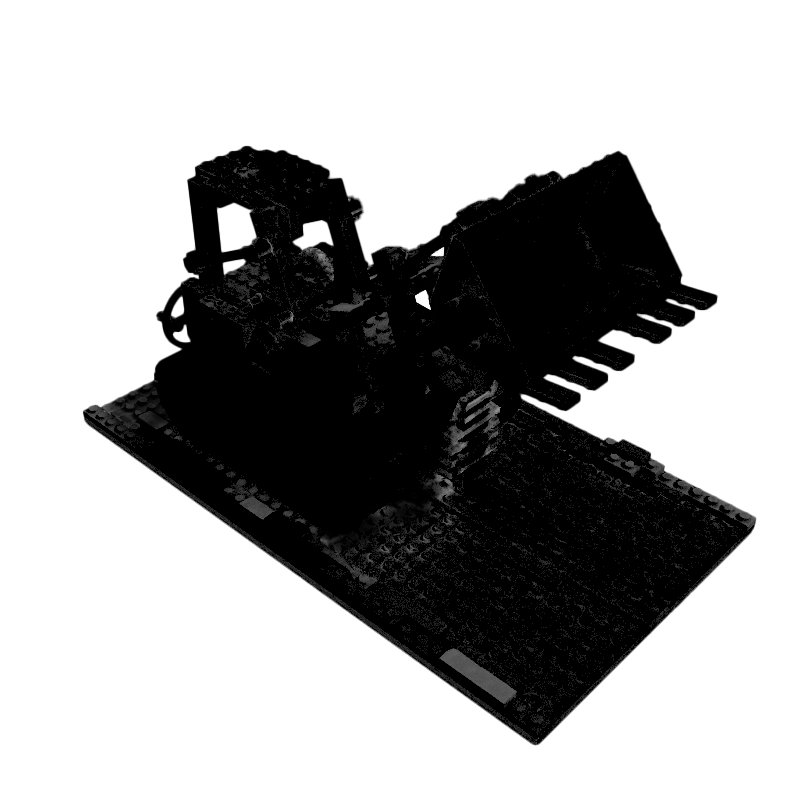
\includegraphics[width=0.22\textwidth]{ch3/specular_show/lego/gloss.png}} &
      \subfloat{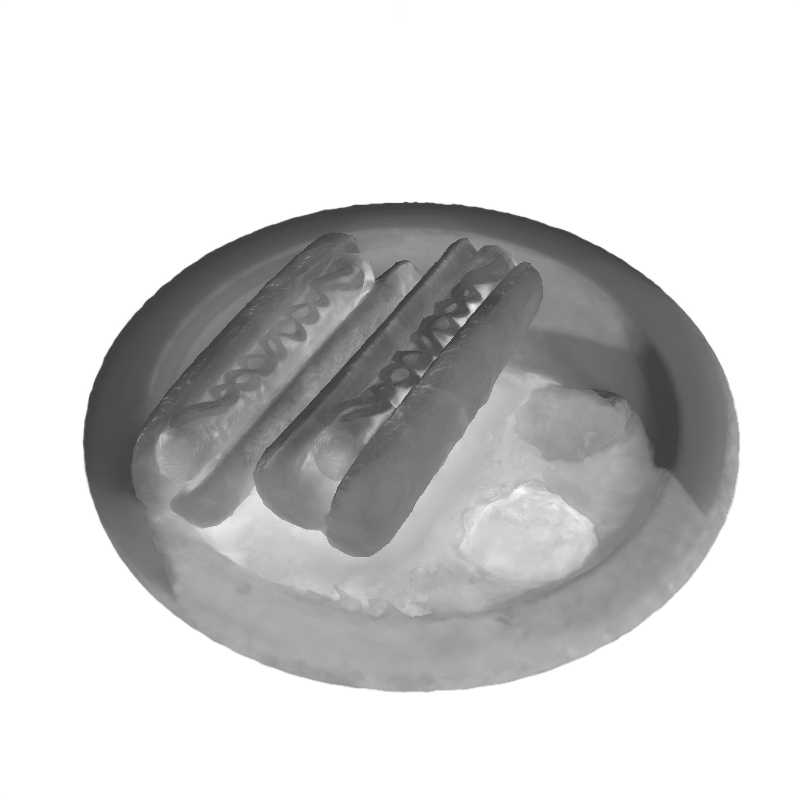
\includegraphics[width=0.22\textwidth]{ch3/specular_show/hotdog/gloss.png}} &
      \subfloat{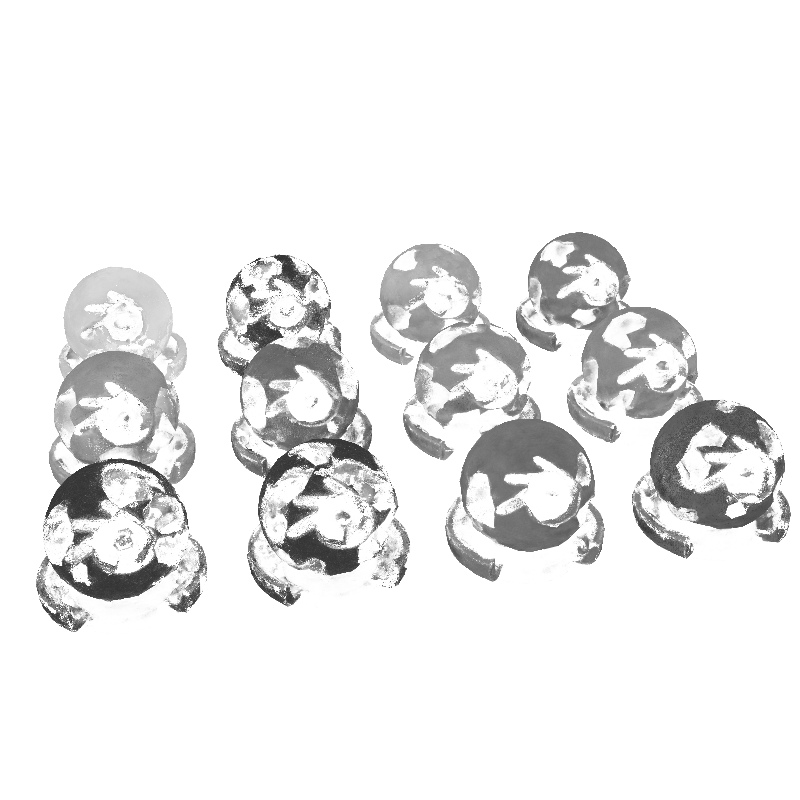
\includegraphics[width=0.22\textwidth]{ch3/specular_show/materials/gloss.png}} &
      \subfloat{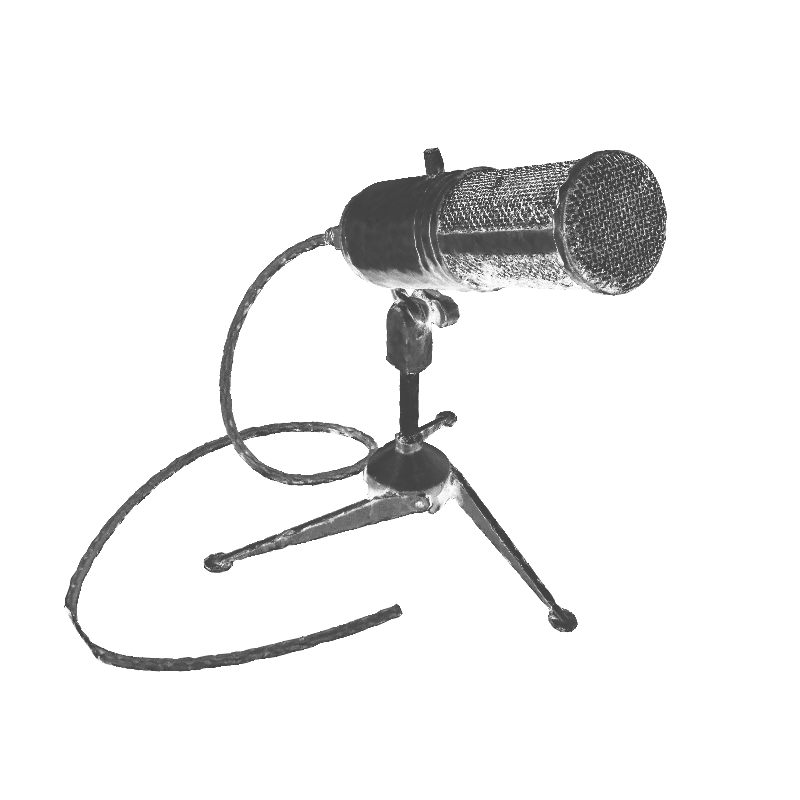
\includegraphics[width=0.22\textwidth]{ch3/specular_show/mic/gloss.png}} \\

  \end{tabular}

  \caption{Specular工作流分解效果}
  \label{fig:specular_show}
\end{figure}

\clearpage

Blinn-Phong工作流分解的实验结果如图\ref{fig:blinn_show}所示。该工作流对应Color、Specular Roll Off和Eccentricity三张纹理。
Color纹理能够控制漫反射的基础颜色,剩余两张纹理则控制高光的形状。由于着色模型的真实感较低,
Blinn-Phong工作流漫反射颜色分解的效果显著低于其它两个工作流,无法区分明暗来自于光照还是表面固有颜色。

\begin{figure}[htbp]
  \centering
  \renewcommand{\arraystretch}{1} % 调整表格行距
  \setlength{\tabcolsep}{3pt} % 调整列间距

  \begin{tabular}{c c c c c} 
      & Lego & Hotdog & Materials & Mic\\

      \raisebox{2.7\height}{\rotatebox[origin=c]{90}{Color}} & % 关键修改
      \subfloat{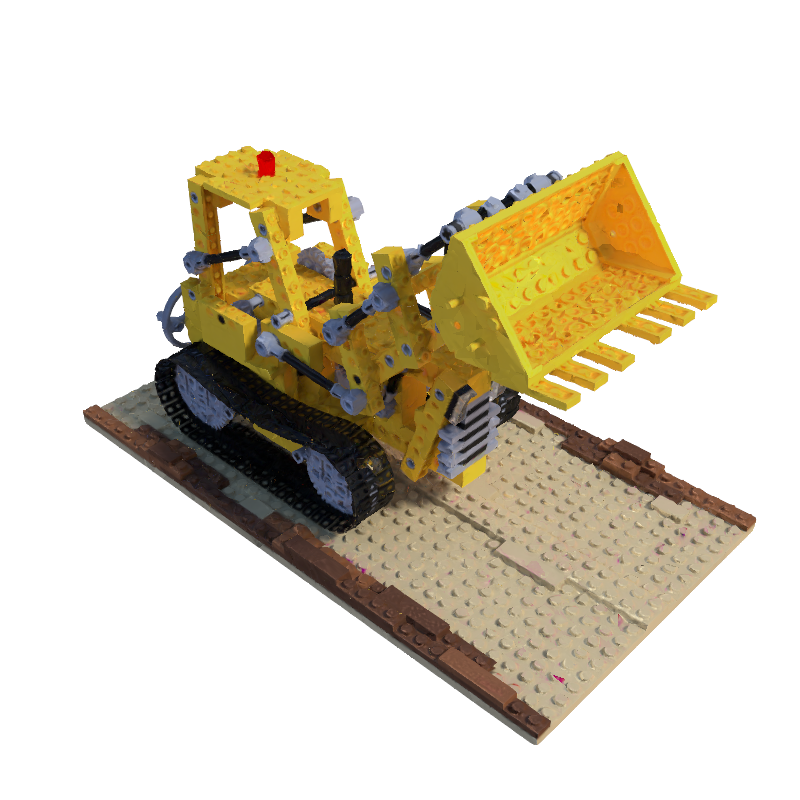
\includegraphics[width=0.22\textwidth]{ch3/blinn_show/lego/kd.png}} &
      \subfloat{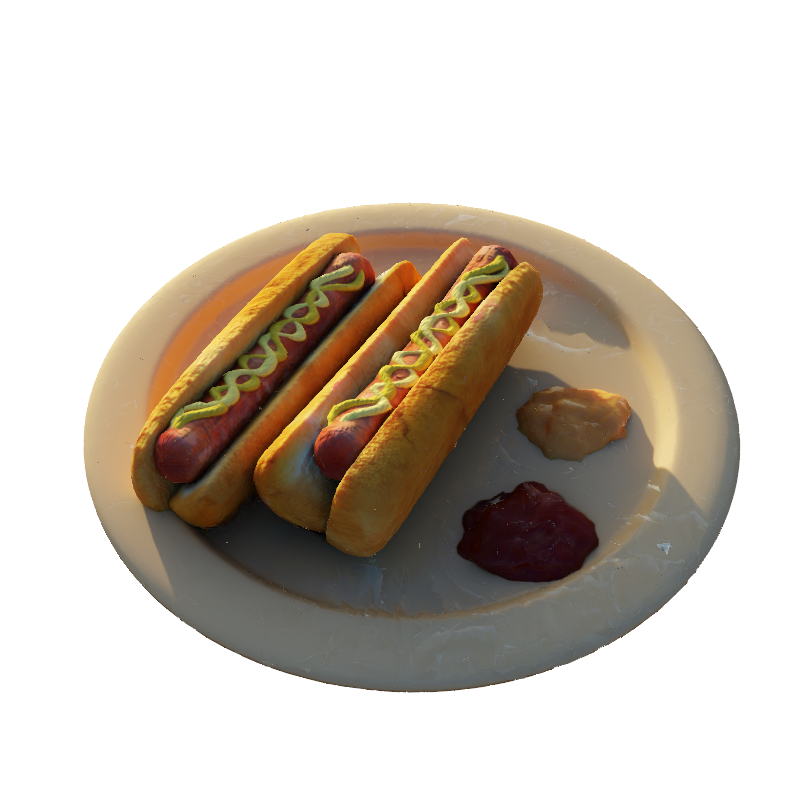
\includegraphics[width=0.22\textwidth]{ch3/blinn_show/hotdog/kd.png}} &
      \subfloat{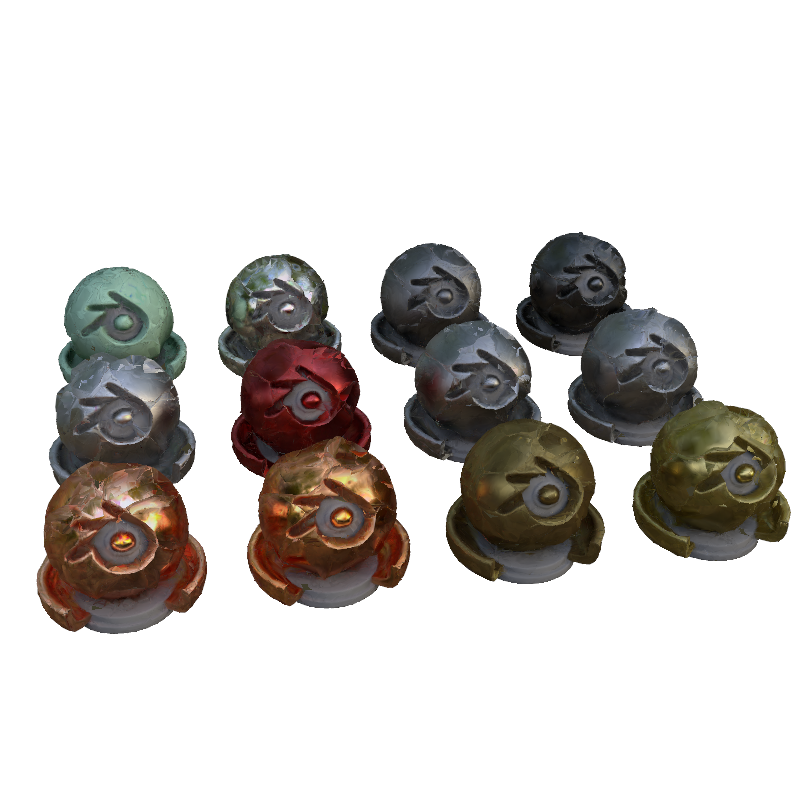
\includegraphics[width=0.22\textwidth]{ch3/blinn_show/materials/kd.png}} &
      \subfloat{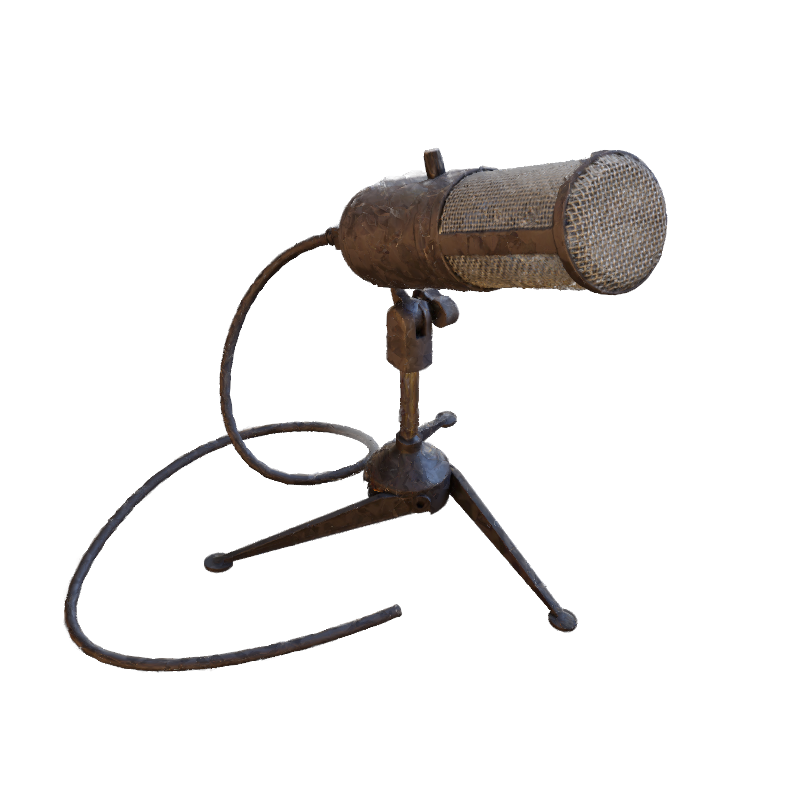
\includegraphics[width=0.22\textwidth]{ch3/blinn_show/mic/kd.png}} \\

      \raisebox{0.5\height}{\rotatebox[origin=c]{90}{Specular Roll Off}} & % 关键修改
      \subfloat{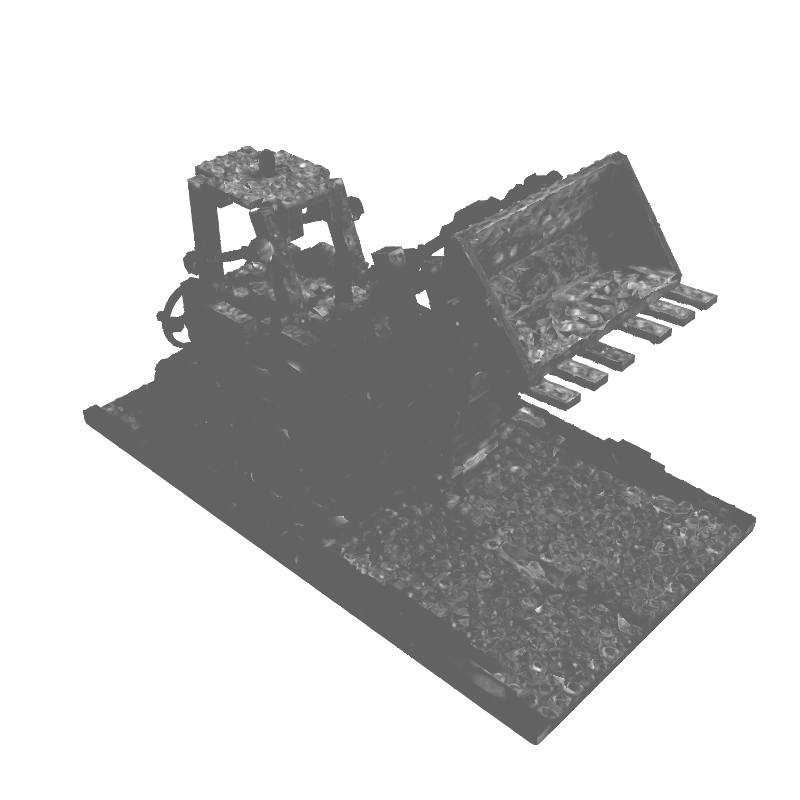
\includegraphics[width=0.22\textwidth]{ch3/blinn_show/lego/spec_roll.png}} &
      \subfloat{\includegraphics[width=0.22\textwidth]{ch3/blinn_show/hotdog/spec_roll.png}} &
      \subfloat{\includegraphics[width=0.22\textwidth]{ch3/blinn_show/materials/spec_roll.png}} &
      \subfloat{\includegraphics[width=0.22\textwidth]{ch3/blinn_show/mic/spec_roll.png}} \\

      \raisebox{1.5\height}{\rotatebox[origin=c]{90}{Eccentricity}} & % 关键修改
      \subfloat{\includegraphics[width=0.22\textwidth]{ch3/blinn_show/lego/ecc.png}} &
      \subfloat{\includegraphics[width=0.22\textwidth]{ch3/blinn_show/hotdog/ecc.png}} &
      \subfloat{\includegraphics[width=0.22\textwidth]{ch3/blinn_show/materials/ecc.png}} &
      \subfloat{\includegraphics[width=0.22\textwidth]{ch3/blinn_show/mic/ecc.png}} \\

  \end{tabular}

  \caption{Blinn-Phong工作流分解效果}
  \label{fig:blinn_show}
\end{figure}

\clearpage

表\ref{tab:rendering_comparison}展示了不同工作流解耦的对比指标,注意到部分场景在不同的工作流中出现了结果略微变化的现象,
本文认为其原因为场景特性与工作流匹配程度不同。例如,对于Lego和Hotdog场景,金属物体较少,反光物体较多,
因此在Specular工作流中表现略好;对于Materials和Mic场景,金属物体占比较多,反射更强烈,因此Metallic工作流表现更好。
另外,Metallic和Specular两种工作流效果在平均值上优于Blinn-Phong工作流,这可能是因为前二者使用了基于物理的着色模型进行渲染,
而Blinn-Phong使用的是经验模型,在渲染技术的真实感上有所不同。
\begin{table}[h]
  \centering
  \caption{不同工作流定量实验结果}
  \begin{tabular}{l ccc ccc ccc}
      \toprule
      & \multicolumn{3}{c}{Metallic} & \multicolumn{3}{c}{Specular} & \multicolumn{3}{c}{Blinn-Phong} \\
      \cmidrule(lr){2-4} \cmidrule(lr){5-7} \cmidrule(lr){8-10}
      & PSNR$\uparrow$ & LPIPS$\downarrow$ & SSIM$\uparrow$ & PSNR$\uparrow$ & LPIPS$\downarrow$ & SSIM$\uparrow$ & PSNR$\uparrow$ & LPIPS$\downarrow$ & SSIM$\uparrow$ \\
      \midrule
      Lego & 28.99 & 0.055 & 0.948 & 29.21 & 0.046 & 0.959 & 28.87 & 0.058 & 0.945 \\
      Hotdog & 33.13 & 0.047 & 0.973 & 35.78 & 0.041 & 0.979 & 31.36 & 0.065 & 0.963 \\
      Materials & 26.39 & 0.077 & 0.929 & 25.62 & 0.078 & 0.914 & 23.39 & 0.119 & 0.881 \\
      Mic & 31.01 & 0.033 & 0.976 & 29.90 & 0.037 & 0.968 & 28.85 & 0.052 & 0.960 \\
      Chair & 31.97 & 0.033 & 0.971 & 31.44 & 0.042 & 0.961 & 29.82 & 0.044 & 0.956 \\
      Drums & 24.55 & 0.078 & 0.922 & 23.61 & 0.083 & 0.910 & 23.80 & 0.082 & 0.916 \\
      Ficus & 24.68 & 0.079 & 0.932 & 24.28 & 0.082 & 0.926 & 24.18 & 0.087 & 0.923 \\
      Ship & 26.17 & 0.168 & 0.824 & 27.74 & 0.176 & 0.801 & 25.40 & 0.183 & 0.806 \\
      \midrule
      Mean & 28.36 & 0.071 & 0.934 & 28.45 & 0.073 & 0.927 & 26.96 & 0.086 & 0.919 \\
      \bottomrule
  \end{tabular}
  \label{tab:rendering_comparison}
\end{table}

实验结果显示,本文所提出的NeRF光照分解管线在处理多种传统工作流资产时表现出优异的解耦效果。
在Lego场景中,通过对复杂几何结构与多色积木构成的挖掘机进行分解,管线不仅成功捕捉到了细微的几何变化,
还精准地反映了在不同光照条件下表面光泽与材质的变化;这证明了方法在复杂结构和动态光照响应上的鲁棒性。
Hotdog场景的实验则表明,该管线能够有效分离出漫反射与镜面反射等不同光照成分,同时保持食物和餐具圆润平滑的几何细节。
Materials场景展示了其在多材质条件下的适用性,通过准确识别金属、塑料和陶瓷等不同材料的反射特性,
实现了精细几何信息的恢复。而在要求更高的Mic场景中,管线仍然能够从微小物体和复杂表面中提取出细致的几何与反射属性,
充分展示了其高效性和适应性。综上所述,这些实验结果全面验证了该方法在各类场景下实现几何与光照反射属性有效解耦的能力,
为传统渲染工作流提供了全新的高效解决方案。

\subsection{分解结果重渲染与编辑实验}

本节实验旨在评估本文提出的光照分解管线的输出结果在传统渲染器以及下游编辑任务中的应用效果。
为了检验其在实际渲染环境中的表现,我们选择了虚幻引擎5.3作为渲染器。虚幻引擎5.3是行业内主流的游戏开发引擎,
广泛用于高质量图形渲染,它支持多种工作流,能够进行离线渲染和即时渲染,且具备出色的渲染效果,
适合对光照和材质细节进行细致分析,实验环境如图\ref{fig:rerender_setup}。

\begin{figure}[htb]
  \centering
  \includegraphics[width=0.8\linewidth]{ch3/rerender_setup.png}
  \caption{重渲染实验环境设置}
  \label{fig:rerender_setup}
\end{figure}

在本实验中,我们使用上一节中提到的实验结果作为数字资产,展示在虚幻引擎中的渲染效果。
每种工作流使用其对应的着色模型作为材质,进行不同视角和光照条件下的重渲染。实验结果证明了
每种工作流分解后的资产均能用于渲染,与传统数字资产具有相同的渲染效果。

其次,为了检验管线输出结果在下游编辑任务中的应用,本课题选择了Maya作为实验平台。
Maya是一款可以对网格体进行精细编辑的软件,是主流的数字资产编辑工具,
与Maya兼容可以证明本文管线输出在传统流程中的适用性。在本实验中,
本文修改了管线的输出的网格体以及贴图纹理,实验结果如图\ref{}所示。

\begin{figure}[htb]
  \centering
  \includegraphics[width=0.8\linewidth]{ch3/maya_setup.png}
  \caption{下游编辑实验环境设置}
  \label{fig:rerender_setup}
\end{figure}

通过这些实验,本文验证了所提出的光照分解管线在传统渲染引擎中的高效性和可应用性,为后续的实际应用提供了坚实的基础。

\section{消融实验}

本节针对不同损失函数进行了定量与定性的消融实验,以证明本文设计的损失函数的有效性,并以此展示其工作原理。图\ref{fig:geo_ablation}为定性的消融实验结果,并分别展示了完整的网格体模型、网格体线框模型、局部细节三种视角。

\begin{figure}[htbp]
  \centering
  \renewcommand{\arraystretch}{1} % 调整表格行距
  \setlength{\tabcolsep}{3pt} % 调整列间距

  \begin{tabular}{c c c} 
      \subfloat{\includegraphics[width=0.3\textwidth]{ch3/geo_ablation/mesh/everything_circle.png}} &
      \subfloat{\includegraphics[width=0.3\textwidth]{ch3/geo_ablation/mesh/wo_normal.png}} &
      \subfloat{\includegraphics[width=0.3\textwidth]{ch3/geo_ablation/mesh/wo_lap.png}} \\

      \subfloat{\includegraphics[width=0.3\textwidth]{ch3/geo_ablation/wired/everything.png}} &
      \subfloat{\includegraphics[width=0.3\textwidth]{ch3/geo_ablation/wired/wo_normal.png}} &
      \subfloat{\includegraphics[width=0.3\textwidth]{ch3/geo_ablation/wired/wo_lap.png}} \\

      \subfloat{\includegraphics[width=0.3\textwidth]{ch3/geo_ablation/detail/everything.png}} &
      \subfloat{\includegraphics[width=0.3\textwidth]{ch3/geo_ablation/detail/wo_normal.png}} &
      \subfloat{\includegraphics[width=0.3\textwidth]{ch3/geo_ablation/detail/wo_lap.png}} \\
      Ours & Ours w/o $\mathcal{L}_{\rm{normal}}$ & Ours w/o $\mathcal{L}_{\rm{laplacian}}$ \\

  \end{tabular}

  \caption{不同损失函数的消融实验结果}
  \label{fig:geo_ablation}
\end{figure}

从线框视角能够清晰地看出,在不添加拉普拉斯平滑正则项时,可能会出现多个顶点过度聚集,以通过不正常的尖锐三角面表达高频细节。在传统渲染器中,这种结构会使得渲染结果出现不正常的突起和高光。本文认为,由于可微渲染中的渲染方式不同于传统光栅化,这样的几何结构反而不会出现视觉瑕疵,因此管线倾向于制造过于聚集的顶点分布。在添加了拉普拉斯正则项后,顶点被有效地分散开来,在总顶点数近似的情况下,能够重建更好的表面细节,同时在渲染时也避免了明显的异常瑕疵。

表\ref{tab:loss_ablation}展示了定性的实验结果。其中,加入了拉普拉斯正则化项及法线平滑正则化项的实验结果在不同指标上均有提升,也同样证明了本文方法的有效性。

\begin{table}[htbp]
  \centering
  \caption{不同损失函数的定量消融实验结果}
  \label{tab:loss_ablation}
  \begin{tabular}{ccc|ccc}
    \toprule
    \multicolumn{3}{c|}{损失函数组合} & \multicolumn{3}{c}{评估指标} \\
    \midrule
    $\mathcal{L}_{normal}$ & $\mathcal{L}_{laplacian}$ & $\mathcal{L}_{color}$ & PSNR$\uparrow$ & LPIPS$\downarrow$ & SSIM$\uparrow$ \\
    \midrule
    \checkmark & & & 0.823 & 0.742 & 0.715 \\
    & \checkmark & & 0.789 & 0.705 & 0.682 \\
    & & \checkmark & 0.802 & 0.721 & 0.693 \\
    & \checkmark & \checkmark & 0.835 & 0.763 & 0.732 \\
    \checkmark & & \checkmark & 0.854 & 0.780 & 0.751 \\
    \checkmark & \checkmark & & 0.846 & 0.771 & 0.739 \\
    \checkmark & \checkmark & \checkmark & \textbf{0.878} & \textbf{0.805} & \textbf{0.778} \\
    \bottomrule
  \end{tabular}
\end{table}

% \begin{table}[h]
%   \centering
%   \caption{不同损失函数的定量消融实验结果}
%   \begin{tabular}{l ccc}
%       \toprule
%       & PSNR$\uparrow$ & LPIPS$\downarrow$ & SSIM$\uparrow$ \\
%       \midrule
%       Ours & 28.99 & 0.055 & 0.948 \\
%       Ours w/o $\mathcal{L}_{normal}$ & 28.38 & 0.063 & 0.941 \\
%       Ours w/o $\mathcal{L}_{laplacian}$ & 27.25 & 0.057 & 0.939 \\
%       \bottomrule
%   \end{tabular}
%   \label{tab:loss_ablation}
% \end{table}

% !TeX root = ../main.tex

\chapter{鸡鸭养殖}

...

\section{画图示例}

TIKZ 画线:

\begin{figure}[htb]
  \centering
  % \subcaptionbox{\label{fig:forward-Kinematic-0}}
  %   {
  %     \begin{tikzpicture}[x=1cm, y=1cm, z=0.6cm]
  %       \draw[line width=2mm] (0,0)  -- (0,2);
  %       \draw[red, line width=1.5mm] (0,2)  -- (0,4.12);
  %       \draw[green, line width=1mm] (0,4.12)  -- (0,5.7);
  %       \draw[blue, line width=0.5mm] (0,5.7)  -- (0, 6.4);
  %     \end{tikzpicture}
  %   }
  \subcaptionbox{\label{fig:forward-Kinematic-1}}
    {
      
\begin{tikzpicture}[scale=0.8, x=1cm, y=1cm, z=0.6cm]
        \draw[line width=2mm] (0,0)  -- (0,2);
        \draw[red, line width=1.5mm] (0,2)  -- (1.5,3.5);
        \draw[green, line width=1mm] (1.5,3.5)  -- (2.6,4.6);
        \draw[blue, line width=0.5mm] (2.6, 4.6)  -- (3.15, 5.15);
      \end{tikzpicture}
    }
  \subcaptionbox{\label{fig:forward-Kinematics-2}}
    {
      
\begin{tikzpicture}[scale=0.8, x=1cm, y=1cm, z=0.6cm]
        \draw[line width=2mm] (0,0)  -- (0,2);
        \draw[red, line width=1.5mm] (0,2)  -- (1.5,3.5);
        \draw[green, line width=1mm] (1.5,3.5)  -- (3,3);
        \draw[blue, line width=0.5mm] (3, 3)  -- (3.75, 2.75);
      \end{tikzpicture}
    }
  \subcaptionbox{\label{fig:forward-Kinematics-3}}
    {
      
\begin{tikzpicture}[scale=0.8, x=1cm, y=1cm, z=0.6cm]
        \draw[line width=2mm] (0,0)  -- (0,2);
        \draw[red, line width=1.5mm] (0,2)  -- (1.5,3.5);
        \draw[green, line width=1mm] (1.5,3.5)  -- (3,3);
        \draw[blue, line width=0.5mm] (3,3)  -- (3.5,2.5);
      \end{tikzpicture}
    }
  \caption{正向动力学}
  \label{fig:forward-Kinematics}
\end{figure}

JavaScript 代码高亮示例:

\begin{lstlisting}[language=JavaScript]
function setup() { // 初始化骨骼结构
  let current = root;
  for(const bone in bones) { // 遍历骨骼(可能存在多个顺序)
    const next = bone.mesh;  current.child = next;  current = next;
  }
}
function draw { // 更新绘制
  while(next) {
    next.update();  next.show();  next = next.child;
  }
}
class Segment { constructor(point, length, angle) {...}  update() { /* 根据父节点更新位置 */ } }
\end{lstlisting}


\subsection{公式示例}

欧拉角转四元数公式:
\begin{equation}
  \begin{aligned}
  \mathbf{q} &= \mathbf{q}_z \mathbf{q}_x \mathbf{q}_y \\
  &={
      \begin{bmatrix}
        \cos(\frac{y}{2})\\0\\0\\\sin(\frac{y}{2})\\
      \end{bmatrix}
    }{
      \begin{bmatrix}
        \cos(\frac{p}{2})\\\sin(\frac{p}{2})\\0\\0\\
      \end{bmatrix}
    }{
      \begin{bmatrix}
        \cos(\frac{r}{2})\\0\\\sin(\frac{r}{2})\\0\\
      \end{bmatrix}
    }\\
  &={
    \begin{bmatrix}
      \cos(\frac{p}{2})\cos(\frac{r}{2})\cos(\frac{y}{2})-\sin(\frac{p}{2})\sin(\frac{r}{2})\sin(\frac{y}{2})\\
      \cos(\frac{p}{2})\cos(\frac{r}{2})\sin(\frac{y}{2})-\cos(\frac{p}{2})\sin(\frac{r}{2})\sin(\frac{y}{2})\\
      \cos(\frac{p}{2})\cos(\frac{r}{2})\sin(\frac{y}{2})+\cos(\frac{p}{2})\sin(\frac{r}{2})\sin(\frac{y}{2})\\
      \cos(\frac{p}{2})\cos(\frac{r}{2})\sin(\frac{y}{2})+\cos(\frac{p}{2})\sin(\frac{r}{2})\sin(\frac{y}{2})\\
    \end{bmatrix}}\\
  \end{aligned}
\end{equation}

四元数转欧拉角时,设 $\mathbf {q} ={\begin{bmatrix}q_{0}&q_{1}&q_{2}&q_{3}\end{bmatrix}}^{T}={\begin{bmatrix}q_{w}&q_{x}&q_{y}&q_{z}\end{bmatrix}}^{T}$,
而求解欧拉角时计算机中的 $arctan$ 与 $arcsin$ 只能获得区间 $(-\frac{\pi}{2},\frac{\pi}{2})$ 的结果,因此使用 $asin$ 替换 $arcsin$,$atan2$ 替换 $arctan$ 函数,
则:

\begin{equation}
\begin{aligned}
  \begin{bmatrix}
    pitch \\ roll \\ yaw 
  \end{bmatrix}}={
    \begin{bmatrix}
      {\mbox{asin}}(-2(q_z q_y - q_x q_w))\\
      {\mbox{atan2}}(2(q_z q_x + q_y q_w), q_z^2 - q_x^2 - q_y^2 + q_w^2)\\
      {\mbox{atan2}}(2(q_x q_y + q_z q_w), -q_z^2 - q_x^2 + q_y^2 + q_w^2)
    \end{bmatrix}
\end{aligned}
\end{equation}

\subsubsection{插值公式}

\begin{equation}
  y=y_{0}+(x-x_{0}){\frac {y_{1}-y_{0}}{x_{1}-x_{0}}}={\frac {y_{0}(x_{1}-x)+y_{1}(x-x_{0})}{x_{1}-x_{0}}}
\end{equation}


\section{养殖算法}

\subsection{为什么呢}

画立方体:

% draw cube
% https://tex.stackexchange.com/questions/29877/need-help-creating-a-3d-cube-from-a-2d-set-of-nodes-in-tikz
\begin{figure}
  \centering
  \subcaptionbox{切分立方体\label{fig:octree-cube}}
    {
      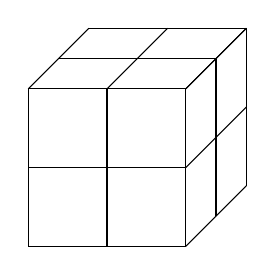
\begin{tikzpicture}
        \foreach \x in{0,...,2}
        {   \draw (0,\x ,2) -- (2,\x ,2);
            \draw (\x ,0,2) -- (\x ,2,2);
            \draw (2,\x ,2) -- (2,\x ,0);
            \draw (\x ,2,2) -- (\x ,2,0);
            \draw (2,0,\x ) -- (2,2,\x );
            \draw (0,2,\x ) -- (2,2,\x );
        }
      \end{tikzpicture}
    }
  \subcaptionbox{对应八叉树\label{fig:octree-tree}}
    {
      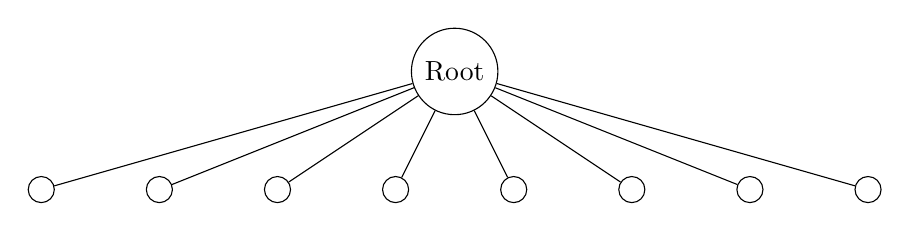
\begin{tikzpicture}
        \tikzstyle{node_style} = [circle,draw=black]
        \node[node_style] {Root}
        child {node[node_style] {}}
        child {node[node_style] {}}
        child {node[node_style] {}}
        child {node[node_style] {}}
        child {node[node_style] {}}
        child {node[node_style] {}}
        child {node[node_style] {}}
        child {node[node_style] {}}
        ;
      \end{tikzpicture}
    }
  \caption{八叉树示例}
  \label{fig:octree}
\end{figure}

放一些看起来高大上的公式。

K-Means 的主要思想是将已知观测集 $(x_1,x_2,...,x_n)$ 划分到 $k$ 个集合($k<=n$),并使每个集合内平方和最小。
即寻找使得下式\eqref{eq:kmeans}最小的聚类 $S_i$($\mu_i$ 是 $S_i$ 中所有点的均值)。
\begin{equation}
  \arg \min_{S_i} \sum_{i=1}^{k} \sum_{x_i \in S_i} (x_i - \mu_i)^2
  \label{eq:kmeans}
\end{equation}

算法实现可主要分为以下两步:分配与更新。

譬如设定存在 $k$ 个初始均值点为 $m_1$,...,$m_k$。

分配:将每个点分配到聚类中,使得集合中的平方和(WCSS)(即平方后的欧式距离)最小。即满足公式\eqref{eq:kmeans_assign}:
\begin{equation}
  S_{i}^{{(t)}}=\left\{x_{p}:\left\|x_{p}-m_{i}^{{(t)}}\right\|^{2}\leq \left\|x_{p}-m_{j}^{{(t)}}\right\|^{2}\forall j,1\leq j\leq k\right\}
  \label{eq:kmeans_assign}
\end{equation}


更新:对于前一步骤得到的每一聚类,重新计算聚类中心(如公式\eqref{eq:kmeans_update}),作为新的均值点。
\begin{equation}
  m_{i}^{{(t+1)}}={\frac  {1}{\left|S_{i}^{{(t)}}\right|}}\sum _{{x_{j}\in S_{i}^{{(t)}}}}x_{j}
  \label{eq:kmeans_update}
\end{equation}


C 代码格式示例:

\begin{lstlisting}[language=c]
  register short *to, *from;
  register count;
  {
    register n = count % 8;
    while (n-- > 0) { 
      *to = *from++;
    }
    n = count / 8;
    if (n == 0) return;     
    do {
      *to = *from++; *to = *from++; *to = *from++; *to = *from++;
      *to = *from++; *to = *from++; *to = *from++; *to = *from++;
    } while (--n > 0)
  }
\end{lstlisting}

三线表:

\begin{table}[h]
  \centering
  \caption{JsPerf (Chrome 84)中循环性能对比}
  \begin{tabular}{p{5cm}p{2cm}}
      \toprule
      \textbf{方法}  & \textbf{Opts/sec} \\
      \midrule
      普通循环 & 165,877  \\
      Duff's Device & 396,801\\
      \bottomrule
  \end{tabular}
  \label{tab:jsperf-efficiency}
\end{table}

\subsubsection{示例图片}

...

多图并列:

\begin{figure}[htbp]
  \centering
  \begin{subfigure}[t]{0.3\textwidth}
  \centering
  \includegraphics[width=.72\textwidth]{yun-kmeans-3.png}
  \caption{K=3}
  \end{subfigure}
  \begin{subfigure}[t]{0.3\textwidth}
  \centering
  \includegraphics[width=.72\textwidth]{yun-kmeans-6.png}
  \caption{K=6}
  \end{subfigure}
  \begin{subfigure}[t]{0.3\textwidth}
  \centering
  \includegraphics[width=.72\textwidth]{yun-kmeans-9.png}
  \caption{K=9}
  \end{subfigure}
  \caption{小云立绘}
  \label{fig:kmeans-png}
\end{figure}


\verb!\href{https://yunyoujun.cn/}{云游君的小站}! 可生成链接\href{https://yunyoujun.cn/}{云游君的小站}。



\section{本章小结}

本章主要介绍...

% !TeX root = ../main.tex

\chapter{总结与展望}

\section{总结}

本文基于NeRF技术开发了一套光照分解管线,旨在解决数字资产与渲染技术之间的耦合问题。
在第3章中,本文结合研究背景和现有方法分析了解耦的目标并选定使用的技术,
设计并实现了数字资产解耦管线。在第4章中,本文根据第3章实验结果中的错误,开展了光照表示的研究。

在数字资产解耦管线的实现方面,本文基于NeRF光照分解相关研究展开工作。
针对现有研究无法将管线输出直接用于传统渲染器以及下游编辑任务的问题,本文采用DMTet结合法线纹理的几何表示方式,
配合正则项的设计,实现了能够直接输出显式网格体的管线。该管线能够无缝对接传统渲染器,扩展了NeRF的下游应用场景。
对于现有研究只能使用单一工作流进行分解的限制,本文设计了MLP纹理,这种设计能够灵活地从多个通道中划分出需要的反射属性,
而且允许管线能够输出纹理贴图。最终,定性定量的实验证明了本文完成了既定目标,成功使用NeRF解除数字资产与渲染技术的耦合。

在光照表示的研究方面,本文从IBL技术对阴影表达能力的欠缺入手,引入了即时渲染中常见的光照组合方式。基于条件输入以及
自动编码器,本文设计了新颖的神经光照表示SANL。SANL能够通过阴影强度结合直接光照与间接光照,
在定量定性实验中展现出优异的性能,使用SANL的光照分解管线在多个数据集上优于其它研究。
本文还通过消融实验进一步揭示了SANL的工作原理,证明了SANL的有效性。

通过以上工作,本文不仅实现了解耦数字资产与渲染技术的目标,在实际应用上展现出价值,并且为光照表示的研究提出了新的可能,
具备理论创新性。

\section{展望}

尽管取得上述成果,但仍有诸多方面值得进一步探索。在未来可能的研究方向中,工业应用和学术扩展是本文工作的重点。

虽然现在的解耦管线已经能够实现直接将输出用于传统渲染器,但是,具体应用上仍有诸多不便。例如,
管线的输入数据还需要估计相机位姿,虽然众多已有方法能够满足这一需求,但是这仍然需要额外的步骤。
未来,数字资产的解耦工作可以进一步地扩展为端到端的管线,直接嵌入传统资产编辑软件,进一步提升实用性。

本文认为,光照分解管线是一个极具潜力的研究方向。虽然本文专注于对数字资产进行分解,但是还有更多方法的输出可以作为本文管线的输入。
比如能够用文本生成图像的人工智能模型,该类模型能够直接输出高质量二维图片,在经过光照分解管线后,可以将产物直接用于渲染引擎,
能够大幅提升数字资产的制作效率。

除了本文现有的应用场景以外,本文管线也可以进一步扩展为按照更复杂的着色模型和工作流进行分解,
比如散射、折射等着色模型。另外,现有即时渲染领域经常使用各类定制的纹理贴图或着色技术以满足特殊效果,
如果本文能够对这些特殊效果进行分解,则不仅能提高特殊效果的开发效率,还能作为新效果的探索和快速验证。

通过以上这些可能的研究方向可以得出,本文的研究仍有极大的潜力。
本文期待能够在渲染和数字资产制作领域发挥更大的作用,助力行业的发展与探索。



% 其他部分
\backmatter

% \titleformat{\chapter}[hang]{\heiti\sanhao\centering}{}{1em}{}{}
\ctexset{
  chapter = {
    format      = \centering\sffamily\sanhao,
  },
}

% 参考文献
\bibliography{ref/refs}  % 参考文献使用 BibTeX 编译
% \printbibliography       % 参考文献使用 BibLaTeX 编译

% 作者简历
% 个人简历、在学期间完成的相关学术成果
% % !TeX root = ../main.tex

\begin{resume}

  % \section*{作者简历}

  % 197× 年 ×× 月 ×× 日出生于四川××县。
  % 1992 年 9 月考入××大学化学系××化学专业,1996 年 7 月本科毕业并获得理学学士学位。
  % 1996 年 9 月免试进入清华大学化学系攻读××化学博士至今。

  % 2019 年 9 月进入中国传媒大学计算机与网络空间安全学院就读计算机应用技术专业数字娱乐与动画技术方向,攻读工学硕士学位。

  % \section*{在学期间所取得的科研成果}

  \subsection*{学术论文}

  \begin{achievements}
    \item 你的论文
  \end{achievements}

  % \subsection*{专利}
  \subsection*{参与软著}

  \begin{achievements}
    \item 你的软著、专利
  \end{achievements}

  \subsection*{参与项目}
  \begin{achievements}
    \item 在学期间参与实验室的项目
  \end{achievements}
\end{resume}


% 致谢
% 盲审时注释掉这里再生成
% % !TeX root = ../main.tex

% 盲审时需删掉,在 main.tex 注释掉即可

\begin{acknowledgements}

  
\end{acknowledgements}
  

% 声明
% \statement
% 将签字扫描后的声明文件 scan-statement.pdf 替换原始页面
% \statement[file=scan-statement.pdf]
% 本科生编译生成的声明页默认不加页脚,插入扫描版时再补上;
% 研究生编译生成时有页眉页脚,插入扫描版时不再重复。
% 也可以手动控制是否加页眉页脚
% \statement[page-style=empty]
% \statement[file=scan-statement.pdf, page-style=plain]



% 指导教师/指导小组学术评语
% % !TeX root = ../main.tex

\begin{comments}
% \begin{comments}[name = {指导小组学术评语}]
% \begin{comments}[name = {Comments from Thesis Supervisor}]
% \begin{comments}[name = {Comments from Thesis Supervision Committee}]

  论文提出了……

\end{comments}


% 答辩委员会决议书
% % !TeX root = ../main.tex

\begin{resolution}

  论文提出了……

  论文取得的主要创新性成果包括:

  1. ……

  2. ……

  3. ……

  论文工作表明作者在×××××具有×××××知识,具有××××能力,论文××××,答辩××××。

  答辩委员会表决,(×票/一致)同意通过论文答辩,并建议授予×××(姓名)×××(门类)学博士/硕士学位。

\end{resolution}


% 本科生的综合论文训练记录表(扫描版)
% \record{file=scan-record.pdf}

\end{document}
